\documentclass[9pt,letterpaper]{book}

\usepackage{latexsym}
\usepackage{amssymb}
\usepackage{amsmath}
\usepackage{bm}
\usepackage{textcomp}
\usepackage{graphicx}
\usepackage{booktabs}
\usepackage{tabularx}
\usepackage{longtable}
\usepackage{ltablex}
\usepackage{wrapfig}
\usepackage[pdfpagemode=None,pdfstartview=FitH,pdfview=FitH,colorlinks=true]%
 {hyperref}

\newtheorem{theorem}{Theorem}[section]
\newcommand{\idx}[1]{{\ensuremath{\mathit{#1}}}}
\newcommand{\qti}{\idx{qti}}
\newcommand{\qtj}{\idx{qtj}}
\newcommand{\pli}{\idx{pli}}
\newcommand{\plj}{\idx{plj}}
\newcommand{\qi}{\idx{qi}}
\newcommand{\ci}{\idx{ci}}
\newcommand{\bmi}{\idx{bmi}}
\newcommand{\bmj}{\idx{bmj}}
\newcommand{\qri}{\idx{qri}}
\newcommand{\qrj}{\idx{qrj}}
\newcommand{\hti}{\idx{hti}}
\newcommand{\sbi}{\idx{sbi}}
\newcommand{\bi}{\idx{bi}}
\newcommand{\bj}{\idx{bj}}
\newcommand{\mbi}{\idx{mbi}}
\newcommand{\mbj}{\idx{mbj}}
\newcommand{\mi}{\idx{mi}}
\newcommand{\cbi}{\idx{cbi}}
\newcommand{\qii}{\idx{qii}}
\newcommand{\ti}{\idx{ti}}
\newcommand{\tj}{\idx{tj}}
\newcommand{\rfi}{\idx{rfi}}
\newcommand{\zzi}{\idx{zzi}}
\newcommand{\ri}{\idx{ri}}
%This somewhat odd construct ensures that \bitvar{\qi}, etc., will set the
% qi in bold face, even though it is in a \mathit font, yet \bitvar{VAR} will
% set VAR in a bold, roman font.
\newcommand{\bitvar}[1]{\ensuremath{\mathbf{\bm{#1}}}}
\newcommand{\locvar}[1]{\ensuremath{\mathrm{#1}}}
\newcommand{\term}[1]{{\em #1}}
\newcommand{\bin}[1]{\ensuremath{\mathtt{b#1}}}
\newcommand{\hex}[1]{\ensuremath{\mathtt{0x#1}}}
\newcommand{\ilog}{\ensuremath{\mathop{\mathrm{ilog}}\nolimits}}
\newcommand{\round}{\ensuremath{\mathop{\mathrm{round}}\nolimits}}
\newcommand{\sign}{\ensuremath{\mathop{\mathrm{sign}}\nolimits}}
\newcommand{\lflim}{\ensuremath{\mathop{\mathrm{lflim}}\nolimits}}

%Section-based table, figure, and equation numbering.
\numberwithin{equation}{chapter}
\numberwithin{figure}{chapter}
\numberwithin{table}{chapter}

\keepXColumns

\pagestyle{headings}
\bibliographystyle{alpha}

\title{Theora I Specification}
\author{Xiph.org Foundation}
\date{\today}


\begin{document}

\frontmatter

\begin{titlepage}
\maketitle
\end{titlepage}
\thispagestyle{empty}
\cleardoublepage

\pagenumbering{roman}

\thispagestyle{plain}
\tableofcontents
\cleardoublepage

\thispagestyle{plain}
\listoffigures
\cleardoublepage

\thispagestyle{plain}
\listoftables
\cleardoublepage

\thispagestyle{plain}
\markboth{{\sc Notation and Conventions}}{{\sc Notation and Conventions}}
\chapter*{Notation and Conventions}

All parameters either passed in or out of a decoding procedure are given in
 \bitvar{bold\ face}.

The prefix \bin{} indicates that the following value is to be interpreted as a
 binary number (base 2).
\begin{verse}
{\bf Example:} The value \bin{1110100} is equal to the decimal value 116.
\end{verse}

The prefix \hex{} indicates the the following value is to be interpreted as a
 hexadecimal number (base 16).
\begin{verse}
{\bf Example:} The value \hex{74} is equal to the decimal value 116.
\end{verse}

All arithmetic defined by this specification is exact.
However, any real numbers that do arise will always be converted back to
 integers again in short order.
The entire specification can be implemented using only normal integer
 operations.
All operations are to be implemented with sufficiently large integers so that
 overflow cannot occur.
Where the result of a computation is to be truncated to a fixed-sized binary
 representation, this will be explicitly noted.
The size given for all variables is the maximum number of bits needed to store
 any value in that variable.
Intermediate computations involving that variable may require more bits.

The following operators are defined:

\begin{description}
\item[$|a|$]
The absolute value of a number $a$.
\begin{align*}
|a| & = \left\{\begin{array}{ll}
-a, & a < 0 \\
a, & a \ge 0
\end{array}\right.
\end{align*}

\item[$a*b$]
Multiplication of a number $a$ by a number $b$.
\item[$\frac{a}{b}$]
Exact division of a number $a$ by a number $b$, producing a potentially
 non-integer result.

\item[$\left\lfloor a\right\rfloor$] 
The largest integer less than or equal to a real number $a$.

\item[$\left\lceil a\right\rceil$]
The smallest integer greater than or equal to a real number $a$.

\item[$a//b$]
Integer division of $a$ by $b$.
\begin{align*}
a//b & = \left\{\begin{array}{ll}
\left\lceil\frac{a}{b}\right\rceil, & a < 0 \\
\left\lfloor\frac{a}{b}\right\rfloor, & a \ge 0
\end{array}\right.
\end{align*}

\item[$a\%b$]
The remainder from the integer division of $a$ by $b$.
\begin{align*}
a\%b & = a-|b|*\left\lfloor\frac{a}{|b|}\right\rfloor
\end{align*}
Note that with this definition, the result is always non-negative and less than
 $|b|$.

\item[$a<<b$]
The value obtained by left-shifting the two's complement integer $a$ by $b$
 bits.
For purposes of this specification, overflow is ignored, and so this is
 equivalent to integer multiplication of $a$ by $2^b$.

\item[$a>>b$]
The value obtained by right-shifting the two's complement integer $a$ by $b$
 bits, filling in the leftmost bits of the new value with $0$ if $a$ is
 non-negative and $1$ if $a$ is negative.
This is {\em not} equivalent to integer division of $a$ by $2^b$.
Instead,
\begin{align*}
a>>b & = \left\lfloor\frac{a}{2^b}\right\rfloor.
\end{align*}

\item[$\round(a)$]
Rounds a number $a$ to the nearest integer, with ties rounded away from $0$.
\begin{align*}
\round(a) = \left\{\begin{array}{ll}
\lceil a-\frac{1}{2}\rceil   & a \le 0 \\
\lfloor a+\frac{1}{2}\rfloor & a > 0
\end{array}\right.
\end{align*}

\item[$\sign(a)$]
Returns the sign of a given number.
\begin{align*}
\sign(a) = \left\{\begin{array}{ll}
-1 & a < 0 \\
0  & a = 0 \\
1  & a > 0
\end{array}\right.
\end{align*}

\item[$\ilog(a)$]
The minimum number of bits required to store a positive integer $a$ in
 two's complement notation, or $0$ for a non-positive integer $a$.
\begin{align*}
\ilog(a) = \left\{\begin{array}{ll}
0, & a \le 0 \\
\left\lfloor\log_2{a}\right\rfloor+1, & a > 0
\end{array}\right.
\end{align*}

\begin{verse}
{\bf Examples:}
\begin{itemize}
\item $\ilog(-1)=0$
\item $\ilog(0)=0$
\item $\ilog(1)=1$
\item $\ilog(2)=2$
\item $\ilog(3)=2$
\item $\ilog(4)=3$
\item $\ilog(7)=3$
\end{itemize}
\end{verse}

\item[$\min(a,b)$]
The minimum of two numbers $a$ and $b$.

\item[$\max(a,b)$]
The maximum of two numbers $a$ and $b$.

\end{description}
\cleardoublepage


\thispagestyle{plain}
\markboth{{\sc Key words}}{{\sc Key words}}
\chapter*{Key words}

%We can't rewrite this, because this is text required by RFC 2119, so we use
% some emergency stretching to get it typeset properly.
\setlength{\emergencystretch}{2em}
The key words ``MUST'', ``MUST NOT'', ``REQUIRED'', ``SHALL'', ``SHALL NOT'',
 ``SHOULD'', ``SHOULD NOT'', ``RECOMMENDED'', ``MAY'', and ``OPTIONAL'' in this
 document are to be intrepreted as described in RFC 2119 \cite{rfc2119}.\par
\setlength{\emergencystretch}{0em}

Where such assertions are placed on the contents of a Theora bitstream itself,
 implementations should be prepared to encounter bitstreams that do not follow
 these requirements.
An application's behavior in the presecence of such non-conforming bitstreams
 is not defined by this specification, but any reasonable method of handling 
 them MAY be used.
By way of example, applications MAY discard the current frame, retain the
 current output thus far, or attempt to continue on by assuming some default
 values for the erroneous bits.
When such an error occurs in the bitstream headers, an application MAY refuse
 to decode the entire stream.
An application SHOULD NOT allow such non-conformant bitstreams to overflow
 buffers and potentially execute arbitrary code, as this represents a serious
 security risk.

An application MUST, however, ensure any bits marked as reserved have the value
 zero, and refuse to decode the stream if they do not.
These are used as place holders for future bitstream features with which the
 current bitstream is forward-compatible.
Such features may not increment the bitstream version number, and can only be
 recognized by checking the value of these reserved bits.

\cleardoublepage



\mainmatter

\pagenumbering{arabic}
\setcounter{page}{1}

\chapter{Introduction}

Theora is a general purpose, lossy video codec.
It is based on the VP3 video codec produced by On2 Technologies
 (\url{http://www.on2.com/}).
On2 donated the VP3.1 source code to the Xiph.org Foundation and released it
 under a BSD-like license.
On2 also made an irrevocable, royalty-free license grant for any patent claims
 it might have over the software and any derivatives.
No formal specification exists for the VP3 format beyond this source code,
 however Mike Melanson maintains a detailed description \cite{Mel04}.
Portions of this specification were adopted from that text with permission.

\section{VP3 and Theora}

Theora contains a superset of the features that were available in the original
 VP3 codec.
Content encoded with VP3.1 can be losslessly transcoded into the Theora format.
Theora content cannot, in general, be losslessly transcoded into the VP3
 format.
If a feature is not available in the original VP3 format, this is mentioned
 when that feature is defined.
A complete list of these features appears in Appendix~\ref{app:vp3-compat}.
%TODO: VP3 - theora comparison in appendix

\section{Video Formats}

Theora I currently supports progressive video data of arbitrary dimensions at a
 constant frame rate in one of several $Y'C_bC_r$ color spaces.
The precise definition the supported color spaces appears in
 Section~\ref{sec:colorspaces}.
Three different chroma subsampling formats are supported: 4:2:0, 4:2:2,
 and 4:4:4.
The precise details of each of these formats and their sampling locations are
 described in Section~\ref{sec:pixfmts}.

The Theora I format does not support interlaced material, variable frame rates,
 bit-depths larger than 8 bits per component, nor alternate color spaces such
 as RGB or arbitrary multi-channel spaces.
Black and white content can be efficiently encoded, however, because the
 uniform chroma planes compress well.
Support for interlaced material is planned for a future version.
\begin{verse}
{\bf Note:} Infrequently changing frame rates---as when film and video
 sequences are cut together---can be supported in the Ogg container format by
 chaining several Theora streams together.
\end{verse}
Support for increased bit depths or additional color spaces is not planned.

\section{Classification}

Theora I is a block-based lossy transform codec that utilizes an
 $8\times 8$ Type-II Discrete Cosine Transform and block-based motion
 compensation.
This places it in the same class of codecs as MPEG-1, -2, -4, and H.263.
The details of how individual blocks are organized and how DCT coefficients are
 stored in the bitstream differ substantially from these codecs, however.
Theora supports only intra frames (I frames in MPEG) and inter frames (P frames
 in MPEG).
There is no equivalent to the bi-predictive frames (B frames) found in MPEG
 codecs.

\section{Assumptions}

The Theora codec design assumes a complex, psychovisually-aware encoder and a
 simple, low-complexity decoder.
%TODO: Talk more about implementation complexity.

Theora provides none of its own framing, synchronization, or protection against
 transmission errors. 
An encoder is solely a method of accepting input video frames and
 compressing these frames into raw, unformatted `packets'.
The decoder then accepts these raw packets in sequence, decodes them, and
 synthesizes a fascimile of the original video frames.
Theora is a free-form variable bit rate (VBR) codec, and packets have no
 minimum size, maximum size, or fixed/expected size.

Theora packets are thus intended to be used with a transport mechanism that
 provides free-form framing, synchronization, positioning, and error correction
 in accordance with these design assumptions, such as Ogg (for file transport)
 or RTP (for network multicast).
For the purposes of a few examples in this document, we will assume that Theora
 is embedded in an Ogg stream specifically, although this is by no means a
 requirement or fundamental assumption in the Theora design.

The specification for embedding Theora into an Ogg transport stream is given in
 Appendix~\ref{app:oggencapsulation}.

\section{Codec Setup and Probability Model}

Theora's heritage is the proprietary commerical codec VP3, and it retains a
 fair amount of inflexibility when compared to Vorbis \cite{vorbis}, the first
 Xiph.org codec, which began as a research codec.
However, to provide additional scope for encoder improvement, Theora adopts
 some of the configurable aspects of decoder setup that are present in Vorbis.
This configuration data is not available in VP3, which uses hardcoded values
 instead.

Theora makes the same controversial design decision that Vorbis made to include
 the entire probability model for the DCT coefficients and all the quantization
 parameters in the bitstream headers.
This is often several hundred fields.
It is therefore impossible to decode any frame in the stream without
 having previously fetched the codec info and codec setup headers.

\begin{verse}
{\bf Note:} Theora {\em can} initiate decode at an arbitrary intra-frame packet
 within a bitstream so long as the codec has been initialized with the setup
 headers.
\end{verse}

Thus, Theora headers are both required for decode to begin and relatively large
 as bitstream headers go.
The header size is unbounded, although as a rule-of-thumb less than 16kB is
 recommended, and Xiph.org's reference encoder follows this suggestion.
%TODO: Is 8kB enough? My setup header is 7.4kB, that doesn't leave much room
% for comments.
%RG: the lesson from vorbis is that as small as possible is really
% important in some applications. Practically, what's acceptable
% depends a great deal on the target bitrate. I'd leave 16 kB in the
% spec for now. fwiw more than 1k of comments is quite unusual.

Our own design work indicates that the primary liability of the required header
 is in mindshare; it is an unusual design and thus causes some amount of
 complaint among engineers as this runs against current design trends and
 points out limitations in some existing software/interface designs.
However, we find that it does not fundamentally limit Theora's suitable
 application space.

%silvia: renamed
%\subsection{Format Specification}
\section{Format Conformance}

The Theora format is well-defined by its decode specification; any encoder that
 produces packets that are correctly decoded by an implementation following
 this specification may be considered a proper Theora encoder.
A decoder must faithfully and completely implement the specification defined
 herein %, except where noted,
 to be considered a conformant Theora decoder.
A decoder need not be implemented strictly as described, but the
 actual decoder process MUST be {\em entirely mathematically equivalent}
 to the described process.
Where appropriate, a non-normative description of encoder processes is
 included.
These sections will be marked as such, and a proper Theora encoder is not
 bound to follow them.

%TODO: \subsection{Hardware Profile}


\chapter{Coded Video Structure}

Theora's encoding and decoding process is based on $8\times 8$ blocks of
 pixels.
This sections describes how a video frame is laid out, divided into
 blocks, and how those blocks are organized.

\section{Frame Layout}

A video frame in Theora is a two-dimensional array of pixels.
Theora, like VP3, uses a right-handed coordinate system, with the origin in the
 lower-left corner of the frame.
This is contrary to many video formats which use a left-handed coordinate
 system with the origin in the upper-left corner of the frame.
%INT: This means that for interlaced material, the definition of `even fields'
%INT:  and `odd fields' may be reversed between Theora and other video codecs.
%INT: This document will always refer to them as `top fields' and `bottom
%INT:  fields'.

Theora divides the pixel array up into three separate \term{color planes}, one
 for each of the $Y'$, $C_b$, and $C_r$ components of the pixel.
The $Y'$ plane is also called the \term{luma plane}, and the $C_b$ and $C_r$
 planes are also called the \term{chroma planes}.
Each plane is assigned a numerical value, as shown in
 Table~\ref{tab:color-planes}.

\begin{table}[htbp]
\begin{center}
\begin{tabular}{cl}\toprule
Index & Color Plane \\\midrule
$0$   & $Y'$        \\
$1$   & $C_b$       \\
$2$   & $C_r$       \\
\bottomrule\end{tabular}
\end{center}
\caption{Color Plane Indices}
\label{tab:color-planes}
\end{table}

In some pixel formats, the chroma planes are subsampled by a factor of two
 in one or both directions.
This means that the width or height of the chroma planes may be half that of
 the total frame width and height.
The luma plane is never subsampled.

\section{Picture Region}

An encoded video frame in Theora is required to have a width and height that
 are multiples of sixteen, making an integral number of blocks even when the
 chroma planes are subsampled.
However, inside a frame a smaller \term{picture region} may be defined
 to present material whose dimensions are not a multiple of sixteen pixels, as
 shown in Figure~\ref{fig:pic-frame}.
The picture region can be offset from the lower-left corner of the frame by up
 to 255 pixels in each direction, and may have an arbitrary width and height,
 provided that it is contained entirely within the coded frame.
It is this picture region that contains the actual video data.
The portions of the frame which lie outside the picture region may contain
 arbitrary image data, so the frame must be cropped to the picture region
 before display.
The picture region plays no other role in the decode process, which operates on
 the entire video frame.

\begin{figure}[htbp]
\begin{center}
\includegraphics{pic-frame}
\end{center}
\caption{Location of frame and picture regions}
\label{fig:pic-frame}
\end{figure}

\section{Blocks and Super Blocks}
\label{sec:blocks-and-sbs}

Each color plane is subdivided into \term{blocks} of $8\times 8$ pixels.
Blocks are grouped into $4\times 4$ arrays called \term{super blocks} as
 shown in Figure~\ref{fig:superblock}.
Each color plane has its own set of blocks and super blocks.
If the chroma planes are subsampled, they are still divided into $8\times 8$
 blocks of pixels; there are just fewer blocks than in the luma plane.
The boundaries of blocks and super blocks in the luma plane do not necessarily
 coincide with those of the chroma planes, if the chroma planes have been
 subsampled.

\begin{figure}[htbp]
\begin{center}
\includegraphics{superblock}
\end{center}
\caption{Subdivision of a frame into blocks and super blocks}
\label{fig:superblock}
\end{figure}

Blocks are accessed in two different orders in the various decoder processes.
The first is \term{raster order}, illustrated in Figure~\ref{fig:raster-block}.
This accesses each block in row-major order, starting in the lower left of the
 frame and continuing along the bottom row of the entire frame, followed by the
 next row up, starting on the left edge of the frame, etc.

\begin{figure}[htbp]
\begin{center}
\includegraphics{raster-block}
\end{center}
\caption{Raster ordering of $n\times m$ blocks}
\label{fig:raster-block}
\end{figure}

The second is \term{coded order}.
In coded order, blocks are accessed by super block.
Within each frame, super blocks are traversed in raster order,
 similar to raster order for blocks.
Within each super block, however, blocks are accessed in a Hilbert curve
 pattern, illustrated in Figure~\ref{fig:hilbert-block}.
If a color plane does not contain a complete super block on the top or right
 sides, the same ordering is still used, simply with any blocks outside the
 frame boundary ommitted.

\begin{figure}[htbp]
\begin{center}
\includegraphics{hilbert-block}
\end{center}
\caption{Hilbert curve ordering of blocks within a super block}
\label{fig:hilbert-block}
\end{figure}

To illustrate this ordering, consider a frame that is 240 pixels wide and
 48 pixels high.
Each row of the luma plane has 30 blocks and 8 super blocks, and there are 6
 rows of blocks and two rows of super blocks.

%When accessed in raster order, each block in the luma plane is assigned the
% following indices:

%\vspace{\baselineskip}
%\begin{center}
%\begin{tabular}{|ccccccc|}\hline
%150 & 151 & 152 & 153 & $\ldots$ & 178 & 179 \\
%120 & 121 & 122 & 123 & $\ldots$ & 148 & 149 \\\hline
% 90 &  91 &  92 &  93 & $\ldots$ & 118 & 119 \\
% 60 &  61 &  62 &  63 & $\ldots$ &  88 &  89 \\
% 30 &  31 &  32 &  33 & $\ldots$ &  58 &  59 \\
%  0 &   1 &   2 &   3 & $\ldots$ &  28 &  29 \\\hline
%\end{tabular}
%\end{center}
%\vspace{\baselineskip}

When accessed in coded order, each block in the luma plane is assigned the
 following indices:

\vspace{\baselineskip}
\begin{center}
\begin{tabular}{|cccc|c|cc|}\hline
123 & 122 & 125 & 124 & $\ldots$ & 179 & 178 \\
120 & 121 & 126 & 127 & $\ldots$ & 176 & 177 \\\hline
  5 &   6 &   9 &  10 & $\ldots$ & 117 & 118 \\
  4 &   7 &   8 &  11 & $\ldots$ & 116 & 119 \\
  3 &   2 &  13 &  12 & $\ldots$ & 115 & 114 \\
  0 &   1 &  14 &  15 & $\ldots$ & 112 & 113 \\\hline
\end{tabular}
\end{center}
\vspace{\baselineskip}

Here the index values specify the order in which the blocks would be accessed.
The indices of the blocks are numbered continuously from one color plane to the
 next.
They do not reset to zero at the start of each plane.
Instead, the numbering increases continuously from the $Y'$ plane to the $C_b$
 plane to the $C_r$ plane.
The implication is that the blocks from all planes are treated as a unit during
 the various processing steps.

Although blocks are sometimes accessed in raster order, in this document the
 index associated with a block is {\em always} its index in coded order.

\section{Macro Blocks}
\label{sec:mbs}

A macro block contains a $2\times 2$ array of blocks in the luma plane
 {\em and} the co-located blocks in the chroma planes, as shown in
 Figure~\ref{fig:macroblock}.
Thus macro blocks can represent anywhere from six to twelve blocks, depending
 on how the chroma planes are subsampled.
This is in contrast to super blocks, which only contain blocks from a single
 color plane.
% the whole super vs. macro blocks thing is a little confusing, and it can be
% hard to remember which is what initially. A figure would/will help here,
% but I tried to add some text emphasizing the difference in terms of
% functionality.
%TBT: At this point we haven't described any functionality yet.
%TBT: As far as the reader knows, the only purpose of the blocks, macro blocks
%TBT:  and super blocks is for data organization---and for blocks and super
%TBT:  blocks, this is essentially true.
%TBT: So lets restrict the differences we emphasize to those of data
%TBT:  organization, which the sentence I just added above does.
Macro blocks contain information about coding mode and motion vectors for the
 corresponding blocks in all color planes.

\begin{figure}[htbp]
 \begin{center}
 \includegraphics{macroblock}
 \end{center}
 \caption{Subdivision of a frame into macro blocks}
 \label{fig:macroblock}
\end{figure}

Macro blocks are also accessed in a \term{coded order}.
This coded order proceeds by examining each super block in the luma plane in
 raster order, and traversing the four macro blocks inside using a smaller
 Hilbert curve, as shown in Figure~\ref{fig:hilbert-mb}.
%r: I rearranged the wording to make a more formal idiom here
If the luma plane does not contain a complete super block on the top or right
 sides, the same ordering is still used, with any macro blocks outside
 the frame boundary simply omitted.
Because the frame size is constrained to be a multiple of 16, there are never
 any partial macro blocks.
Unlike blocks, macro blocks need never be accessed in a pure raster order.

\begin{figure}[htbp]
\begin{center}
\includegraphics{hilbert-mb}
\end{center}
\caption{Hilbert curve ordering of macro blocks within a super block}
\label{fig:hilbert-mb}
\end{figure}

Using the same frame size as the example above, there are 15 macro blocks in
 each row and 3 rows of macro blocks.
The macro blocks are assigned the following indices:

\vspace{\baselineskip}
\begin{center}
\begin{tabular}{|cc|cc|c|cc|c|}\hline
30 & 31 & 32 & 33 & $\cdots$ & 42 & 43 & 44 \\\hline
 1 &  2 &  5 &  6 & $\cdots$ & 25 & 26 & 29 \\
 0 &  3 &  4 &  7 & $\cdots$ & 24 & 27 & 28 \\\hline
\end{tabular}
\end{center}
\vspace{\baselineskip}

\section{Coding Modes and Prediction}

Each block is coded using one of a small, fixed set of \term{coding modes} that
 define how the block is predicted from previous frames.
A block is predicted using one of two \term{reference frames}, selected
 according to the coding mode.
A reference frame is the fully decoded version of a previous frame in the
 stream.
The first available reference frame is the previous intra frame, called the
 \term{golden frame}.
The second available reference frame is the previous frame, whether it was an
 intra frame or an inter frame.
If the previous frame was an intra frame, then both reference frames are the
 same.
See Figure~\ref{fig:reference-frames} for an illustration of the reference
 frames used for an intra frame that does not follow an intra frame.

\begin{figure}[htbp]
\begin{center}
\includegraphics{reference-frames}
\end{center}
\caption{Example of reference frames for an inter frame}
\label{fig:reference-frames}
\end{figure}

Two coding modes in particular are worth mentioning here.
The INTRA mode is used for blocks that are not predicted from either reference
 frame.
This is the only coding mode allowed in intra frames.
The INTER\_NOMV coding mode uses the co-located contents of the block in the
 previous frame as the predictor.
This is the default coding mode.

\section{DCT Coefficients}
\label{sec:dct-coeffs}

A \term{residual} is added to the predicted contents of a block to form the
 final reconstruction.
The residual is stored as a set of quantized coefficients from an integer
 approximation of a two-dimensional Type II Discrete Cosine Transform.
The DCT takes an $8\times 8$ array of pixel values as input and returns an
 $8\times 8$ array of coefficient values.
The \term{natural ordering} of these coefficients is defined to be row-major
 order, from lowest to highest frequency.
They are also often indexed in \term{zig-zag order}, as shown in
 Figure~\ref{tab:zig-zag}.

\begin{figure}[htbp]
\begin{center}
\begin{tabular}[c]{rr|c@{}c@{}c@{}c@{}c@{}c@{}c@{}c@{}c@{}c@{}c@{}c@{}c@{}c@{}c}
 &\multicolumn{1}{r}{} & && &&&&&$c$&&& && &&  \\
 &\multicolumn{1}{r}{} &0&&1&&2&&3&&4&&5&&6&&7 \\\cline{3-17}
 &0 &  0 &$\rightarrow$&  1 &&  5 &$\rightarrow$&  6 && 14 &$\rightarrow$& 15 && 27 &$\rightarrow$& 28            \\[-0.5\defaultaddspace]
 &  &    &$\swarrow$&&$\nearrow$& &$\swarrow$&&$\nearrow$& &$\swarrow$&&$\nearrow$& &$\swarrow$&                  \\
 &1 &  2 &             &  4 &&  7 &             & 13 && 16 &             & 26 && 29 &             & 42            \\[-0.5\defaultaddspace]
 &  &$\downarrow$&$\nearrow$&&$\swarrow$&&$\nearrow$&&$\swarrow$&&$\nearrow$&&$\swarrow$&&$\nearrow$&$\downarrow$ \\
 &2 &  3 &             &  8 && 12 &             & 17 && 25 &             & 30 && 41 &             & 43            \\[-0.5\defaultaddspace]
 &  &    &$\swarrow$&&$\nearrow$& &$\swarrow$&&$\nearrow$& &$\swarrow$&&$\nearrow$& &$\swarrow$&                  \\
 &3 &  9 &             & 11 && 18 &             & 24 && 31 &             & 40 && 44 &             & 53            \\[-0.5\defaultaddspace]
$r$&&$\downarrow$&$\nearrow$&&$\swarrow$&&$\nearrow$&&$\swarrow$&&$\nearrow$&&$\swarrow$&&$\nearrow$&$\downarrow$ \\
 &4 & 10 &             & 19 && 23 &             & 32 && 39 &             & 45 && 52 &             & 54            \\[-0.5\defaultaddspace]
 &  &    &$\swarrow$&&$\nearrow$& &$\swarrow$&&$\nearrow$& &$\swarrow$&&$\nearrow$& &$\swarrow$&                  \\
 &5 & 20 &             & 22 && 33 &             & 38 && 46 &             & 51 && 55 &             & 60            \\[-0.5\defaultaddspace]
 &  &$\downarrow$&$\nearrow$&&$\swarrow$&&$\nearrow$&&$\swarrow$&&$\nearrow$&&$\swarrow$&&$\nearrow$&$\downarrow$ \\
 &6 & 21 &             & 34 && 37 &             & 47 && 50 &             & 56 && 59 &             & 61            \\[-0.5\defaultaddspace]
 &  &    &$\swarrow$&&$\nearrow$& &$\swarrow$&&$\nearrow$& &$\swarrow$&&$\nearrow$& &$\swarrow$&                  \\
 &7 & 35 &$\rightarrow$& 36 && 48 &$\rightarrow$& 49 && 57 &$\rightarrow$& 58 && 62 &$\rightarrow$& 63
\end{tabular}
\end{center}
\caption{Zig-zag order}
\label{tab:zig-zag}
\end{figure}

\begin{verse}
{\bf Note:} the row and column indices refer to {\em frequency number} and not
 pixel locations.
The frequency numbers are defined independently of the memory organization of
 the pixels.
They have been written from top to bottom here to follow conventional notation,
 despite the right-handed coordinate system Theora uses for pixel locations.
%RG: I'd rather we were internally consistent and put dc at the lower left.
Many implementations of the DCT operate `in-place'.
That is, they return DCT coefficients in the same memory buffer that the
 initial pixel values were stored in.
Due to the right-handed coordinate system used for pixel locations in Theora,
 one must note carefully how both pixel values and DCT coefficients are
 organized in memory in such a system.
\end{verse}

DCT coefficient $(0,0)$ is called the \term{DC coefficient}.
All the other coefficients are called \term{AC coefficients}.


\chapter{Decoding Overview}

This section provides a high level description of the Theora codec's
 construction.
A bit-by-bit specification appears beginning in Section~\ref{sec:bitpacking}.
The later sections assume a high-level understanding of the Theora decode
 process, which is provided below.

\section{Decoder Configuration}

Decoder setup consists of configuration of the quantization matrices and the
 Huffman codebooks for the DCT coefficients, and a table of limit values for
 the deblocking filter.
The remainder of the decoding pipeline is not configurable.

\subsection{Global Configuration}

The global codec configuration consists of a few video related fields, such as
 frame rate, frame size, picture size and offset, aspect ratio, color space,
 pixel format, and a version number.
The version number is divided into a major version, a minor version, amd a
 minor revision number.
%r: afaik the released vp3 codec called itself 3.1 and is compatible w/ theora
%r: even though we received the in-progress 3.2 codebase
For the format defined in this specification, these are `3', `2', and
 `0', respectively, in reference to Theora's origin as a successor to the VP3.1
 format.

\subsection{Quantization Matrices}

Theora allows up to 384 different quantization matrices to be defined, one for
 each \term{quantization type}, \term{color plane} ($Y'$, $C_b$, or $C_r$), and
 \term{quantization index}, \qi, which ranges from zero to 63, inclusive.
There are currently two quantization types defined, which depend on the coding
 mode of the block being dequantized, as shown in Table~\ref{tab:quant-types}.

\begin{table}[htbp]
\begin{center}
\begin{tabular}{cl}\toprule
Quantization Type & Usage                     \\\midrule
$0$               & INTRA-mode blocks         \\
$1$               & Blocks in any other mode. \\
\bottomrule\end{tabular}
\end{center}
\caption{Quantization Type Indices}
\label{tab:quant-types}
\end{table}

%r: I think 'nominally' is more specific than 'generally' here
The quantization index, on the other hand, nominally represents a progressive
 range of quality levels, from low quality near zero to high quality near 63.
However, the interpretation is arbitrary, and it is possible, for example, to
 partition the scale into two completely separate ranges with 32 levels each
 that are meant to represent different classes of source material, or any
 other arrangement that suits the encoder's requirements.

Each quantization matrix is an $8\times 8$ matrix of 16-bit values, which is
 used to quantize the output of the $8\times 8$ DCT\@.
Quantization matrices are specified using three components: a
 \term{base matrix} and two \term{scale values}.
The first scale value is the \term{DC scale}, which is applied to the DC
 component of the base matrix.
The second scale value is the \term{AC scale}, which is applied to all the
 other components of the base matrix.
There are 64 DC scale values and 64 AC scale values, one for each \qi\ value.

There are 64 elements in each base matrix, one for each DCT coefficient.
They are stored in natural order (cf. Section~\ref{sec:dct-coeffs}).
There is a separate set of base matrices for each quantization type and each
 color plane, with up to 64 possible base matrices in each set, one for each
 \qi\ value.
%r: we will mention that the given matricies must bound the \qi range
%r: in the detailed section. it's not important at this level.
Typically the bitstream contains matrices for only a sparse subset of the
 possible \qi\ values.
The base matrices for the remainder of the \qi\ values are computed using
 linear interpolation.
This configuration allows the encoder to adjust the quantization matrices to
 approximate the complex, non-linear response of the human visual system to
 different quantization errors.

Finally, because the in-loop deblocking filter strength depends on the strength
 of the quantization matrices defined in this header, a table of 64 \term{loop
 filter limit values} is defined, one for each \qi\ value.

The precise specification of how all of this information is decoded appears in
 Section~\ref{sub:loop-filter-limits} and Section~\ref{sub:quant-params}.

\subsection{Huffman Codebooks}

Theora uses 80 configurable binary Huffman codes to represent the 32 tokens
 used to encode DCT coefficients.
Each of the 32 token values has a different semantic meaning and is used to
 represent single coefficient values, zero runs, combinations of the two, and
 \term{End-Of-Block markers}.

The 80 codes are divided up into five groups of 16, with each group
 corresponding to a set of DCT coefficient indices.
The first group corresponds to the DC coefficient, while the remaining four
 groups correspond to different subsets of the AC coefficients.
Within each frame, two pairs of 4-bit codebook indices are stored.
The first pair selects which codebooks to use from the DC coefficient group for
 the $Y'$ coefficients and the $C_b$ and $C_r$ coefficients.
The second pair selects which codebooks to use from {\em all four} of the AC
 coefficient groups for the $Y'$ coefficients and the $C_b$ and $C_r$
 coefficients.

The precise specification of how the codebooks are decoded appears in
 Section~\ref{sub:huffman-tables}.

\section{High-Level Decode Process}

\subsection{Decoder Setup}

Before decoding can begin, a decoder MUST be initialized using the bitstream
 headers corresponding to the stream to be decoded.
Theora uses three header packets; all are required, in order, by this
 specification.
Once set up, decode may begin at any intra-frame packet---or even inter-frame
 packets, provided the appropriate decoded reference frames have already been
 decoded and cached---belonging to the Theora stream.
In Theora I, all packets after the three initial headers are intra-frame or
 inter-frame packets.

The header packets are, in order, the identification header, the comment
 header, and the setup header.

\paragraph{Identification Header}

The identification header identifies the stream as Theora, provides a version
 number, and defines the characteristics of the video stream such as frame
 size.
A complete description of the identification header appears in
 Section~\ref{sec:idheader}.

\paragraph{Comment Header}

The comment header includes user text comments (`tags') and a vendor string
 for the application/library that produced the stream.
The format of the comment header is the same as that used in the Vorbis I and
 Speex codecs, with slight modifications due to the use of a different bit
 packing mechanism.
A complete description of how the comment header is coded appears in
 Section~\ref{sec:commentheader}, along with a suggested set of tags.

\paragraph{Setup Header}

The setup header includes extensive codec setup information, including the
 complete set of quantization matrices and Huffman codebooks needed to decode
 the DCT coefficients.
A complete description of the setup header appears in
 Section~\ref{sec:setupheader}.

\subsection{Decode Procedure}

The decoding and synthesis procedure for all video packets is fundamentally the
 same, with some steps omitted for intra frames.
\begin{itemize}
\item
Decode packet type flag.
\item
Decode frame header.
\item
Decode coded block information (inter frames only).
\item
Decode macro block mode information (inter frames only).
\item
Decode motion vectors (inter frames only).
\item
Decode block-level \qi\ information.
\item
Decode DC coefficient for each coded block.
\item
Decode 1st AC coefficient for each coded block.
\item
Decode 2nd AC coefficient for each coded block.
\item
$\ldots$
\item
Decode 63rd AC coefficient for each coded block.
\item Perform DC coefficient prediction.
\item Reconstruct coded blocks.
\item Copy uncoded bocks.
\item Perform loop filtering.
\end{itemize}

\begin{verse}
{\bf Note:} clever rearrangement of the steps in this process is possible.
As an example, in a memory-constrained environment, one can make multiple
 passes through the DCT coefficients to avoid buffering them all in memory.
On the first pass, the starting location of each coefficient is identified, and
 then 64 separate get pointers are used to read in the 64 DCT coefficients
 required to reconstruct each coded block in sequence.
This operation produces entirely equivalent output and is naturally perfectly
 legal.
It may even be a benefit in non-memory-constrained environments due to a
 reduced cache footprint.
\end{verse}

Theora makes equivalence easy to check by defining all decoding operations in
 terms of exact integer operations.
No floating-point math is required, and in particular, the implementation of
 the iDCT transform MUST be followed precisely.
This prevents the decoder mismatch problem commonly associated with codecs that
 provide a less rigorous transform specification.
Such a mismatch problem would be devastating to Theora, since a single rounding
 error in one frame could propagate throughout the entire succeeding frame due
 to DC prediction.

\paragraph{Packet Type Decode}

Theora I uses four packet types.
The first three packet types mark each of the three Theora headers described
 above.
The fourth packet type marks a video packet.
All other packet types are reserved; packets marked with a reserved type should
 be ignored.

Additionally, zero-length packets are treated as if they were an inter 
frame with no blocks coded. That is, as a duplicate frame.

\paragraph{Frame Header Decode}

The frame header contains some global information about the current frame.
The first is the frame type field, which specifies if this is an intra frame or
 an inter frame.
Inter frames predict their contents from previously decoded reference frames.
Intra frames can be independently decoded with no established reference frames.

The next piece of information in the frame header is the list of \qi\ values
 allowed in the frame.
Theora allows from one to three different \qi\ values to be used in a single
 frame, each of which selects a set of six quantization matrices, one for each
 quantization type (inter or intra), and one for each color plane.
The first \qi\ value is {\em always} used when dequantizing DC coefficients.
The \qi\ value used when dequantizing AC coefficients, however, can vary from
 block to block.
VP3, in contrast, only allows a single \qi\ value per frame for both the DC and
 AC coefficients.

\paragraph{Coded Block Information}

This stage determines which blocks in the frame are coded and which are
 uncoded.
A \term{coded block list} is constructed which lists all the coded blocks in
 coded order.
For intra frames, every block is coded, and so no data needs to be read from
 the packet.

\paragraph{Macro Block Mode Information}

For intra frames, every block is coded in INTRA mode, and this stage is
 skipped.
In inter frames a \term{coded macro block list} is constructed from the coded
 block list.
Any macro block which has at least one of its luma blocks coded is considered
 coded; all other macro blocks are uncoded, even if they contain coded chroma
 blocks.
A coding mode is decoded for each coded macro block, and assigned to all its
 constituent coded blocks.
All coded chroma blocks in uncoded macro blocks are assigned the INTER\_NOMV
 coding mode.

\paragraph{Motion Vectors}

Intra frames are coded entirely in INTRA mode, and so this stage is skipped.
Some inter coding modes, however, require one or more motion vectors to be
 specified for each macro block.
These are decoded in this stage, and an appropriate motion vector is assigned
 to each coded block in the macro block.

\paragraph{Block-Level \qi\ Information}

If a frame allows multiple \qi\ values, the \qi\ value assigned to each block
 is decoded here.
Frames that use only a single \qi\ value have nothing to decode.

\paragraph{DCT Coefficients}

Finally, the quantized DCT coefficients are decoded.
A list of DCT coefficients in zig-zag order for a single block is represented
 by a list of tokens.
A token can take on one of 32 different values, each with a different semantic
 meaning.
A single token can represent a single DCT coefficient, a run of zero
 coefficients within a single block, a combination of a run of zero
 coefficients followed by a single non-zero coefficient, an
 \term{End-Of-Block marker}, or a run of EOB markers.
EOB markers signify that the remainder of the block is one long zero run.
Unlike JPEG and MPEG, there is no requirement for each block to end with 
 a special marker.
If non-EOB tokens yield values for all 64 of the coefficients in a block, then
 no EOB marker occurs.

Each token is associated with a specific \term{token index} in a block.
For single-coefficient tokens, this index is the zig-zag index of the token in
 the block.
For zero-run tokens, this index is the zig-zag index of the {\em first}
 coefficient in the run.
For combination tokens, the index is again the zig-zag index of the first
 coefficient in the zero run.
For EOB markers, which signify that the remainder of the block is one long zero
 run, the index is the zig-zag index of the first zero coefficient in that run.
For EOB runs, the token index is that of the first EOB marker in the run.
Due to zero runs and EOB markers, a block does not have to have a token for
 every zig-zag index.

Tokens are grouped in the stream by token index, not by the block they
 originate from.
This means that for each zig-zag index in turn, the tokens with that index from
 {\em all} the coded blocks are coded in coded block order.
When decoding, a current token index is maintained for each coded block.
This index is advanced by the number of coefficients that are added to the
 block as each token is decoded.
After fully decoding all the tokens with token index \ti, the current token
 index of every coded block will be \ti\ or greater.

If an EOB run of $n$ blocks is decoded at token index \ti, then it ends the
 next $n$ blocks in coded block order whose current token index is equal to
 \ti, but not greater.
If there are fewer than $n$ blocks with a current token index of \ti, then the
 decoder goes through the coded block list again from the start, ending blocks
 with a current token index of $\ti+1$, and so on, until $n$ blocks have been
 ended.

Tokens are read by parsing a Huffman code that depends on \ti\ and the color
 plane of the next coded block whose current token index is equal to \ti, but
 not greater.
The Huffman codebooks are selected on a per-frame basis from the 80 codebooks
 defined in the setup header.
Many tokens have a fixed number of \term{extra bits} associated with them.
These bits are read from the packet immediately after the token is decoded.
These are used to define things such as coefficient magnitude, sign, and the
 length of runs.

\paragraph{DC Prediction}

After the coefficients for each block are decoded, the quantized DC value of
 each block is adjusted based on the DC values of its neighbors.
This adjustment is performed by scanning the blocks in raster order, not coded
 block order.

\paragraph{Reconstruction}

Finally, using the coding mode, motion vector (if applicable), quantized
 coefficient list, and \qi\ value defined for each block, all the coded blocks
 are reconstructed.
The DCT coefficients are dequantized, an inverse DCT transform is applied, and
 the predictor is formed from the coding mode and motion vector and added to
 the result.

\paragraph{Loop Filtering}

To complete the reconstructed frame, an ``in-loop'' deblocking filter is
 applied to the edges of all coded blocks.


\chapter{Video Formats}

This section gives a precise description of the video formats that Theora is
 capable of storing.
The Theora bitstream is capable of handling video at any arbitrary resolution
 up to $1048560\times 1048560$.
Such video would require almost three terabytes of storage per frame for
 uncompressed data, so compliant decoders MAY refuse to decode images with
 sizes beyond their capabilities.
%TODO: What MUST a "compliant" decoder accept?
%TODO: What SHOULD a decoder use for an upper bound? (derive from total amount
%TODO:  of memory and memory bandwidth)
%TODO: Any lower limits?
%TODO: We really need hardware device profiles, but such things should be
%TODO:  developed with input from the hardware community.
%TODO: And even then sometimes they're useless

The remainder of this section talks about two specific aspects of the video
 format: the color space and the pixel format.
The first describes how color is represented and how to transform that color
 representation into a device independent color space such as CIE $XYZ$ (1931).
The second describes the various schemes for sampling the color values in time
 and space.

\section{Color Space Conventions}

There are a large number of different color standards used in digital video.
Since Theora is a lossy codec, it restricts itself to only a few of them to
 simplify playback.
Unlike the alternate method of describing all the parameters of the color
 model, this allows a few dedicated routines for color conversion to be written
 and heavily optimized in a decoder.
More flexible conversion functions should instead be specified in an encoder,
 where additional computational complexity is more easily tolerated.
The color spaces were selected to give a fair representation of color standards
 in use around the world today.
Most of the standards that do not exactly match one of these can be converted
 to one fairly easily.

All Theora color spaces are $Y'C_bC_r$ color spaces with one luma channel and
 two chroma channels.
Each channel contains 8-bit discrete values in the range $0\ldots255$, which
 represent non-linear gamma pre-corrected signals.
The Theora identification header contains an 8-bit value that describes the
 color space.
This merely selects one of the color spaces available from an enumerated list.
Currently, only two color spaces are defined, with a third possibility that
 indicates the color space is ``unknown".

\section{Color Space Conversions and Parameters}
\label{sec:color-xforms}

The parameters which describe the conversions between each color space are
 listed below.
These are the parameters needed to map colors from the encoded $Y'C_bC_r$
 representation to the device-independent color space CIE $XYZ$ (1931).
These parameters define abstract mathematical conversion functions which are
 infinitely precise.
The accuracy and precision with which the conversions are performed in a real
 system is determined by the quality of output desired and the available
 processing power.
Exact decoder output is defined by this specification only in the original
 $Y'C_bC_r$ space.

\begin{description}
\item[$Y'C_bC_r$ to $Y'P_bP_r$:]
\vspace{\baselineskip}\hfill

This conversion takes 8-bit discrete values in the range $[0\ldots255]$ and
 maps them to real values in the range $[0\ldots1]$ for Y and
 $[-\frac{1}{2}\ldots\frac{1}{2}]$ for $P_b$ and $P_r$.
Because some values may fall outside the offset and excursion defined for each
 channel in the $Y'C_bC_r$ space, the results may fall outside these ranges in
 $Y'P_bP_r$ space.
No clamping should be done at this stage.

\begin{align}
Y'_\mathrm{out} & =
 \frac{Y'_\mathrm{in}-\mathrm{Offset}_Y}{\mathrm{Excursion}_Y} \\
P_b             & =
 \frac{C_b-\mathrm{Offset}_{C_b}}{\mathrm{Excursion}_{C_b}} \\
P_r             & =
 \frac{C_r-\mathrm{Offset}_{C_r}}{\mathrm{Excursion}_{C_r}}
\end{align}

Parameters: $\mathrm{Offset}_{Y,C_b,C_r}$, $\mathrm{Excursion}_{Y,C_b,C_r}$.

\item[$Y'P_bP_r$ to $R'G'B'$:]
\vspace{\baselineskip}\hfill

This conversion takes the one luma and two chroma channel representation and
 maps it to the non-linear $R'G'B'$ space used to drive actual output devices.
Values should be clamped into the range $[0\ldots1]$ after this stage.

\begin{align}
R' & = Y'+2(1-K_r)P_r \\
G' & = Y'-2\frac{(1-K_b)K_b}{1-K_b-K_r}P_b-2\frac{(1-K_r)K_r}{1-K_b-K_r}P_r\\
B' & = Y'+2(1-K_b)P_b
\end{align}

Parameters: $K_b,K_r$.

\item[$R'G'B'$ to $RGB$ (Output device gamma correction):]
\vspace{\baselineskip}\hfill

This conversion takes the non-linear $R'G'B'$ voltage levels and maps them to
 linear light levels produced by the actual output device.
Note that this conversion is only that of the output device, and its inverse is
 {\em not} that used by the input device.
Because a dim viewing environment is assumed in most television standards, the
 overall gamma between the input and output devices is usually around $1.1$ to
 $1.2$, and not a strict $1.0$.

For calibration with actual output devices, the model
\begin{align}
L & =(E'+\Delta)^\gamma
\end{align}
 should be used, with $\Delta$ the free parameter and $\gamma$ held fixed to
 the value specified in this document.
The conversion function presented here is an idealized version with $\Delta=0$.

\begin{align}
R & = R'^\gamma \\
G & = G'^\gamma \\
B & = B'^\gamma
\end{align}

Parameters: $\gamma$.

\item[$RGB$ to $R'G'B'$ (Input device gamma correction):]
\vspace{\baselineskip}\hfill

%TODO: Tag section as non-normative

This conversion takes linear light levels and maps them to the non-linear
 voltage levels produced in the actual input device.
This information is merely informative.
It is not required for building a decoder or for converting between the various
 formats and the actual output capabilities of a particular device.

A linear segment is introduced on the low end to reduce noise in dark areas of
 the image.
The rest of the scale is adjusted so that the power segment of the curve
 intersects the linear segment with the proper slope, and so that it still maps
 0 to 0 and 1 to 1.

\begin{align}
R' & = \left\{
\begin{array}{ll}
\alpha R,                     & 0\le R<\delta   \\
(1+\epsilon)R^\beta-\epsilon, & \delta\le R\le1
\end{array}\right. \\
G' & = \left\{
\begin{array}{ll}
\alpha G,                     & 0\le G<\delta   \\
(1+\epsilon)G^\beta-\epsilon, & \delta\le G\le1
\end{array}\right. \\
B' & = \left\{
\begin{array}{ll}
\alpha B,                     & 0\le B<\delta   \\
(1+\epsilon)B^\beta-\epsilon, & \delta\le B\le1
\end{array}\right.
\end{align}

Parameters: $\beta$, $\alpha$, $\delta$, $\epsilon$.

\item[$RGB$ to CIE $XYZ$ (1931):]
\vspace{\baselineskip}\hfill

This conversion maps a device-dependent linear RGB space to the
 device-independent linear CIE $XYZ$ space.
The parameters are the CIE chromaticity coordinates of the three
 primaries---red, green, and blue---as well as the chromaticity coordinates
 of the white point of the device.
This is how hardware manufacturers and standards typically describe a
 particular $RGB$ space.
The math required to convert these parameters into a useful transformation
 matrix is reproduced below.

\begin{align}
F                  & =
\left[\begin{array}{ccc}
\frac{x_r}{y_r}       & \frac{x_g}{y_g}       & \frac{x_b}{y_b}       \\
1                     & 1                     & 1                     \\
\frac{1-x_r-y_r}{y_r} & \frac{1-x_g-y_g}{y_g} & \frac{1-x_b-y_b}{y_b}
\end{array}\right] \\
\left[\begin{array}{c}
s_r \\
s_g \\
s_b
\end{array}\right] & =
F^{-1}\left[\begin{array}{c}
\frac{x_w}{y_w} \\
1 \\
\frac{1-x_w-y_w}{y_w}
\end{array}\right] \\
\left[\begin{array}{c}
X \\
Y \\
Z
\end{array}\right] & =
F\left[\begin{array}{c}
s_rR \\
s_gG \\
s_bB
\end{array}\right]
\end{align}
Parameters: $x_r,x_g,x_b,x_w, y_r,y_g,y_b,y_w$.

\end{description}

\section{Available Color Spaces}
\label{sec:colorspaces}

These are the color spaces currently defined for use by Theora video.
Each one has a short name, with which it is referred to in this document, and
 a more detailed specification of the standards from which its parameters are
 derived.
Some standards do not specify all the parameters necessary.
For these unspecified parameters, this document serves as the definition of
 what should be used when encoding or decoding Theora video.

\subsection{Rec.~470M (Rec.~ITU-R~BT.470-6 System M/NTSC with
 Rec.~ITU-R~BT.601-5)}
\label{sec:470m}

This color space is used by broadcast television and DVDs in much of the
 Americas, Japan, Korea, and the Union of Myanmar \cite{rec470}.
This color space may also be used for System M/PAL (Brazil), with an
 appropriate conversion supplied by the encoder to compensate for the
 different gamma value.
See Section~\ref{sec:470bg} for an appropriate gamma value to assume for M/PAL
 input.

In the US, studio monitors are adjusted to a D65 white point
 ($x_w,y_w=0.313,0.329$).
In Japan, studio monitors are adjusted to a D white of 9300K
 ($x_w,y_w=0.285,0.293$).

Rec.~470 does not specify a digital encoding of the color signals.
For Theora, Rec.~ITU-R~BT.601-5 \cite{rec601} is used, starting from the
 $R'G'B'$ signals specified by Rec.~470.

Rec.~470 does not specify an input gamma function.
For Theora, the Rec.~709 \cite{rec709} input function is assumed.
This is the same as that specified by SMPTE 170M \cite{smpte170m}, which claims
 to reflect modern practice in the creation of NTSC signals circa 1994.

The parameters for all the color transformations defined in
 Section~\ref{sec:color-xforms} are given in Table~\ref{tab:470m}.

\begin{table}[htb]
\begin{align*}
\mathrm{Offset}_{Y,C_b,C_r}    & = (16, 128, 128)  \\
\mathrm{Excursion}_{Y,C_b,C_r} & = (219, 224, 224) \\
K_r                            & = 0.299           \\
K_b                            & = 0.114           \\
\gamma                         & = 2.2             \\
\beta                          & = 0.45            \\
\alpha                         & = 4.5             \\
\delta                         & = 0.018           \\
\epsilon                       & = 0.099           \\
x_r,y_r                        & = 0.67, 0.33      \\
x_g,y_g                        & = 0.21, 0.71      \\
x_b,y_b                        & = 0.14, 0.08      \\
\text{(Illuminant C) } x_w,y_w & = 0.310, 0.316    \\
\end{align*}
\caption{Rec.~470M Parameters}
\label{tab:470m}
\end{table}

\subsection{Rec.~470BG (Rec.~ITU-R~BT.470-6 Systems B and G with
 Rec.~ITU-R~BT.601-5)}
\label{sec:470bg}

This color space is used by the PAL and SECAM systems in much of the rest of
 the world \cite{rec470}
This can be used directly by systems (B, B1, D, D1, G, H, I, K, N)/PAL and (B,
 D, G, H, K, K1, L)/SECAM\@.

\begin{verse}
{\bf Note:} the Rec.~470BG chromaticity values are different from those
 specified in Rec.~470M\@.
When PAL and SECAM systems were first designed, they were based upon the same
 primaries as NTSC\@.
However, as methods of making color picture tubes have changed, the primaries
 used have changed as well.
The U.S. recommends using correction circuitry to approximate the existing,
 standard NTSC primaries.
Current PAL and SECAM systems have standardized on primaries in accord with
 more recent technology.
\end{verse}

Rec.~470 provisionally permits the use of the NTSC chromaticity values (given
 in Section~\ref{sec:470m}) with legacy PAL and SECAM equipment.
In Theora, material must be decoded assuming the new PAL and SECAM primaries.
Material intended for display on old legacy devices should be converted by the
 decoder.

The official Rec.~470BG specifies a gamma value of $\gamma=2.8$.
However, in practice this value is unrealistically high \cite{Poyn97}.
Rec.~470BG states that the overall system gamma should be approximately
 $\gamma\beta=1.2$.
Since most cameras pre-correct with a gamma value of $\beta=0.45$,
 this suggests an output device gamma of approximately $\gamma=2.67$.
This is the value recommended for use with PAL systems in Theora.

Rec.~470 does not specify a digital encoding of the color signals.
For Theora, Rec.~ITU-R~BT.601-5 \cite{rec601} is used, starting from the
 $R'G'B'$ signals specified by Rec.~470.

Rec.~470 does not specify an input gamma function.
For Theora, the Rec 709 \cite{rec709} input function is assumed.

The parameters for all the color transformations defined in
 Section~\ref{sec:color-xforms} are given in Table~\ref{tab:470bg}.

\begin{table}[htb]
\begin{align*}
\mathrm{Offset}_{Y,C_b,C_r}    & = (16, 128, 128)  \\
\mathrm{Excursion}_{Y,C_b,C_r} & = (219, 224, 224) \\
K_r                            & = 0.299           \\
K_b                            & = 0.114           \\
\gamma                         & = 2.67            \\
\beta                          & = 0.45            \\
\alpha                         & = 4.5             \\
\delta                         & = 0.018           \\
\epsilon                       & = 0.099           \\
x_r,y_r                        & = 0.64, 0.33      \\
x_g,y_g                        & = 0.29, 0.60      \\
x_b,y_b                        & = 0.15, 0.06      \\
\text{(D65) } x_w,y_w          & = 0.313, 0.329    \\
\end{align*}
\caption{Rec.~470BG Parameters}
\label{tab:470bg}
\end{table}

\section{Pixel Formats}
\label{sec:pixfmts}

Theora supports several different pixel formats, each of which uses different
 subsampling for the chroma planes relative to the luma plane.
A decoder may need to recover a full resolution chroma plane with samples
 co-sited with the luma plane in order to convert to RGB for display or perform
 other processing.
Decoders can assume that the chroma signal satisfies the Nyquist-Shannon
 sampling theorem.
The ideal low-pass reconstruction filter this implies is not practical, but any
 suitable approximation can be used, depending on the available computing
 power.
Decoders MAY simply use a box filter, assigning to each luma sample the chroma
 sample closest to it.
Encoders would not go wrong in assuming that this will be the most common
 approach.

\subsection{4:4:4 Subsampling}
\label{sec:444}

All three color planes are stored at full resolution---each pixel has a $Y'$,
 a $C_b$ and a $C_r$ value (see Figure~\ref{fig:pixel444}).
The samples in the different planes are all at co-located sites.

\begin{figure}[htbp]
\begin{center}
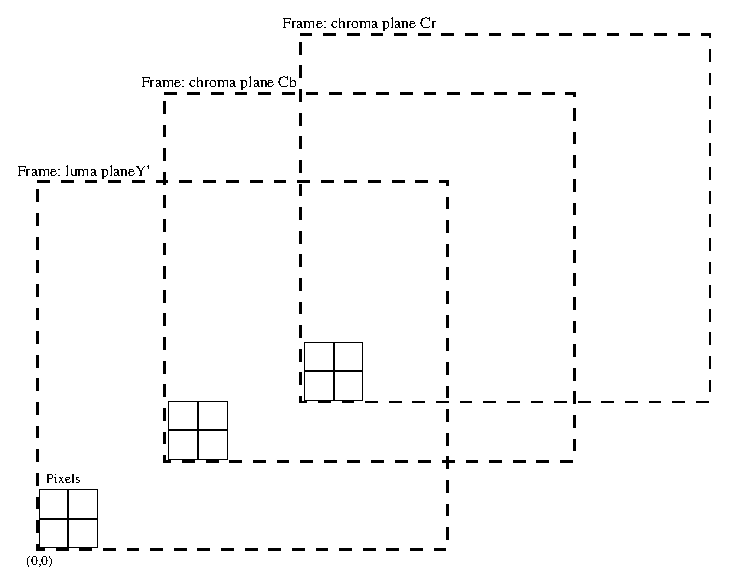
\includegraphics{pixel444}
\end{center}
\caption{Pixels encoded 4:4:4}
\label{fig:pixel444}
\end{figure}

% Figure.
%YRB         YRB
%
%
%
%YRB         YRB
%
%
%


\subsection{4:2:2 Subsampling}
\label{sec:422}

The $C_b$ and $C_r$ planes are stored with half the horizontal resolution of
 the $Y'$ plane.
Thus, each of these planes has half the number of horizontal blocks as the luma
 plane (see Figure~\ref{fig:pixel422}).
Similarly, they have half the number of horizontal super blocks, rounded up.
Macro blocks are defined across color planes, and so their number does not
 change, but each macro block contains half as many chroma blocks.

The chroma samples are vertically aligned with the luma samples, but
 horizontally centered between two luma samples.
Thus, each luma sample has a unique closest chroma sample.
A horizontal phase shift may be required to produce signals which use different
 horizontal chroma sampling locations for compatibility with different systems.

\begin{figure}[htbp]
\begin{center}
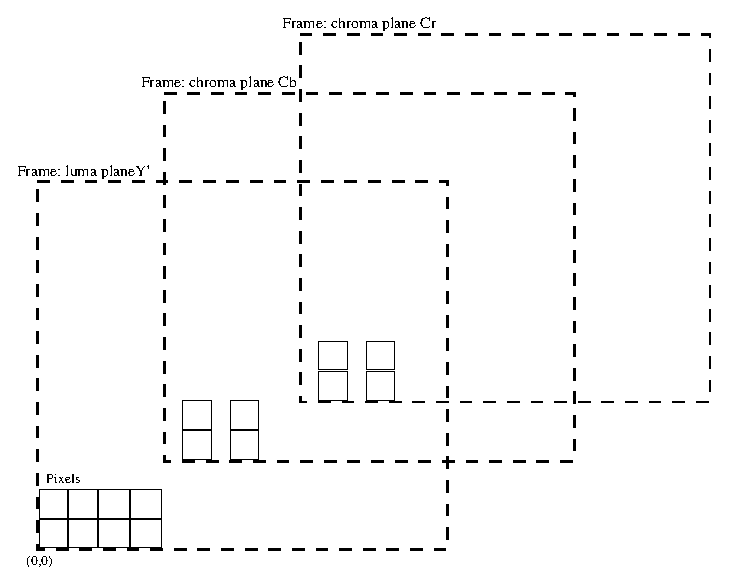
\includegraphics{pixel422}
\end{center}
\caption{Pixels encoded 4:2:2}
\label{fig:pixel422}
\end{figure}

% Figure.
%Y     RB    Y           Y     RB    Y
%
%
%
%Y     RB    Y           Y     RB    Y
%
%
%

\subsection{4:2:0 Subsampling}
\label{sec:420}

The $C_b$ and $C_r$ planes are stored with half the horizontal and half the
 vertical resolution of the $Y'$ plane.
Thus, each of these planes has half the number of horizontal blocks and half
 the number of vertical blocks as the luma plane, for a total of one quarter
 the number of blocks (see Figure~\ref{fig:pixel420}).
Similarly, they have half the number of horizontal super blocks and half the
 number of vertical super blocks, rounded up.
Macro blocks are defined across color planes, and so their number does not
 change, but each macro block contains within it one quarter as many 
 chroma blocks.

The chroma samples are vertically and horizontally centered between four luma
 samples.
Thus, each luma sample has a unique closest chroma sample.
This is the same sub-sampling pattern used with JPEG, MJPEG, and MPEG-1, and
 was inherited from VP3.
A horizontal or vertical phase shift may be required to produce signals which
 use different chroma sampling locations for compatibility with different
 systems.

\begin{figure}[htbp]
\begin{center}
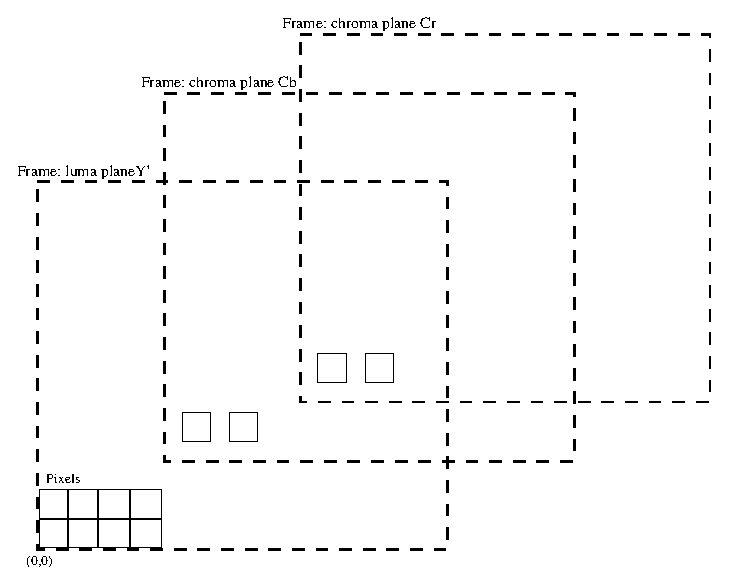
\includegraphics{pixel420}
\end{center}
\caption{Pixels encoded 4:2:0}
\label{fig:pixel420}
\end{figure}

% Figure.
%Y           Y           Y           Y
%
%      RB                      RB
%
%Y           Y           Y           Y
%
%
%
%Y           Y           Y           Y
%
%      RB                      RB
%
%Y           Y           Y           Y
%
%
%

\subsection{Subsampling and the Picture Region}

Although the frame size must be an integral number of macro blocks, and thus
 both the number of pixels and the number of blocks in each direction must be
 even, no such requirement is made of the picture region.
Thus, when using subsampled pixel formats, careful attention must be paid to
 which chroma samples correspond to which luma samples.

As mentioned above, for each pixel format, there is a unique chroma sample that
 is the closest to each luma sample.
When cropping the chroma planes to the picture region, all the chroma samples
 corresponding to a luma sample in the cropped picture region must be included.
Thus, when dividing the width or height of the picture region by two to obtain
 the size of the subsampled chroma planes, they must be rounded up.

Furthermore, the sampling locations are defined relative to the frame,
 {\em not} the picture region.
When using the 4:2:2 and 4:2:0 formats, the locations of chroma samples
 relative to the luma samples depends on whether or not the X offset of the
 picture region is odd.
If the offset is even, each column of chroma samples corresponds to two columns
 of luma samples (see Figure~\ref{fig:pic_even} for an example).
The only exception is if the width is odd, in which case the last column
 corresponds to only one column of luma samples (see Figure~\ref{fig:pic_even_odd}).
If the offset is odd, then the first column of chroma samples corresponds to
 only one column of luma samples, while the remaining columns each correspond
 to two (see Figure~\ref{fig:pic_odd}).
In this case, if the width is even, the last column again corresponds to only
 one column of luma samples (see Figure~\ref{fig:pic_odd_even}).

A similar process is followed with the rows of a picture region of odd height
 encoded in the 4:2:0 format.
If the Y offset is even, each row of chroma samples corresponds to two rows of
 luma samples (see Figure~\ref{fig:pic_even}), except with an odd height, where
 the last row corresponds to one row of chroma luna samples only (see 
 Figure~\ref{fig:pic_even_odd}).
If the offset is odd, then it is the first row of chroma samples which
 corresponds to only one row of luma samples, while the remaining rows each
 correspond to two (Figure~\ref{fig:pic_odd}), except with an even height, 
 where the last row also corresponds to one (Figure~\ref{fig:pic_odd_even}).

Encoders should be aware of these differences in the subsampling when using an
 even or odd offset.
In the typical case, with an even width and height, where one expects two rows
 or columns of luma samples for every row or column of chroma samples, the
 encoder must take care to ensure that the offsets used are both even.

\begin{figure}[htbp]
\begin{center}
\includegraphics[width=\textwidth]{pic_even}
\end{center}
\caption{Pixel correspondence between color planes with even picture 
 offset and even picture size}
\label{fig:pic_even}
\end{figure}

\begin{figure}[htbp]
\begin{center}
\includegraphics[width=\textwidth]{pic_even_odd}
\end{center}
\caption{Pixel correspondence with even picture offset and 
 odd picture size}
\label{fig:pic_even_odd}
\end{figure}

\begin{figure}[htbp]
\begin{center}
\includegraphics[width=\textwidth]{pic_odd}
\end{center}
\caption{Pixel correspondence with odd picture offset and 
 odd picture size}
\label{fig:pic_odd}
\end{figure}

\begin{figure}[htbp]
\begin{center}
\includegraphics[width=\textwidth]{pic_odd_even}
\end{center}
\caption{Pixel correspondence with odd picture offset and 
 even picture size}
\label{fig:pic_odd_even}
\end{figure}


\chapter{Bitpacking Convention}
\label{sec:bitpacking}

\section{Overview}

The Theora codec uses relatively unstructured raw packets containing
 binary integer fields of arbitrary width.
Logically, each packet is a bitstream in which bits are written one-by-one by
 the encoder and then read one-by-one in the same order by the decoder.
Most current binary storage arrangements group bits into a native storage unit
 of eight bits (octets), sixteen bits, thirty-two bits, or less commonly other
 fixed sizes.
The Theora bitpacking convention specifies the correct mapping of the logical
 packet bitstream into an actual representation in fixed-width units.

\subsection{Octets and Bytes}

In most contemporary architectures, a `byte' is synonymous with an `octect',
 that is, eight bits.
For purposes of the bitpacking convention, a byte implies the smallest native
 integer storage representation offered by a platform.
Modern file systems invariably offer bytes as the fundamental atom of storage.

The most ubiquitous architectures today consider a `byte' to be an octet.
Note, however, that the Theora bitpacking convention is still well defined for
 any native byte size; an implementation can use the native bit-width of a
 given storage system.
This document assumes that a byte is one octet for purposes of example only.

\subsection{Words and Byte Order}

A `word' is an integer size that is a grouped multiple of the byte size.
Most architectures consider a word to be a group of two, four, or eight bytes.
Each byte in the word can be ranked by order of `significance', e.g.\ the
 significance of the bits in each byte when storing a binary integer in the
 word.
Several byte orderings are possible in a word.
The common ones are
\begin{itemize}
\item{Big-endian:}
in which the most significant byte comes first, e.g.\ 3-2-1-0,
\item{Little-endian:}
in which the least significant byte comes first, e.g.\ 0-1-2-3, and
\item{Mixed-endian:}
one of the less-common orderings that cannot be put into the above two
 categories, e.g.\ 3-1-2-0 or 0-2-1-3.
\end{itemize}

The Theora bitpacking convention specifies storage and bitstream manipulation
 at the byte, not word, level.
Thus host word ordering is of a concern only during optimization, when writing
 code that operates on a word of storage at a time rather than a byte.
Logically, bytes are always encoded and decoded in order from byte zero through
 byte $n$.

\subsection{Bit Order}

A byte has a well-defined `least significant' bit (LSb), which is the only bit
 set when the byte is storing the two's complement integer value $+1$.
A byte's `most significant' bit (MSb) is at the opposite end.
Bits in a byte are numbered from zero at the LSb to $n$ for the MSb, where
 $n=7$ in an octet.

\section{Coding Bits into Bytes}

The Theora codec needs to encode arbitrary bit-width integers from zero to 32
 bits wide into packets.
These integer fields are not aligned to the boundaries of the byte
 representation; the next field is read at the bit position immediately
 after the end of the previous field.

The decoder logically unpacks integers by first reading the MSb of a binary
 integer from the logical bitstream, followed by the next most significant
 bit, etc., until the required number of bits have been read.
When unpacking the bytes into bits, the decoder begins by reading the MSb of
 the integer to be read from the most significant unread bit position of the
 source byte, followed by the next-most significant bit position of the
 destination integer, and so on up to the requested number of bits.
Note that this differs from the Vorbis I codec, which
 begins decoding with the LSb of the source integer, reading it from the
 LSb of the source byte.
When all the bits of the current source byte are read, decoding continues with
 the MSb of the next byte.
Any unfilled bits in the last byte of the packet MUST be cleared to zero by the
 encoder.

\subsection{Signedness}

The binary integers decoded by the above process may be either signed or
 unsigned.
This varies from integer to integer, and this specification
 indicates how each value should be interpreted as it is read.
That is, depending on context, the three bit binary pattern \bin{111} can be
 taken to represent either `$7$' as an unsigned integer or `$-1$' as a signed,
 two's complement integer.

\subsection{Encoding Example}

The following example shows the state of an (8-bit) byte stream after several
 binary integers are encoded, including the location of the put pointer for the
 next bit to write to and the total length of the stream in bytes.

Encode the 4 bit unsigned integer value `12' (\bin{1100}) into an empty byte
 stream.

\begin{tabular}{r|ccccccccl}
\multicolumn{1}{r}{}& &&&&$\downarrow$&&&& \\
         & 7 & 6 & 5 & 4 & 3 & 2 & 1 & 0 & \\\cline{1-9}
byte 0   & \textbf{1} & \textbf{1} & \textbf{0} & \textbf{0} &
                           0 & 0 & 0 & 0 & $\leftarrow$     \\
byte 1   & 0 & 0 & 0 & 0 & 0 & 0 & 0 & 0 &                  \\
byte 2   & 0 & 0 & 0 & 0 & 0 & 0 & 0 & 0 &                  \\
byte 3   & 0 & 0 & 0 & 0 & 0 & 0 & 0 & 0 &                  \\
\multicolumn{1}{c|}{$\vdots$}&\multicolumn{8}{c}{$\vdots$}& \\
byte $n$ & 0 & 0 & 0 & 0 & 0 & 0 & 0 & 0 &
byte stream length: 1 byte
\end{tabular}
\vspace{\baselineskip}

Continue by encoding the 3 bit signed integer value `-1' (\bin{111}).

\begin{tabular}{r|ccccccccl}
\multicolumn{1}{r}{} &&&&&&&&$\downarrow$& \\
         & 7 & 6 & 5 & 4 & 3 & 2 & 1 & 0 & \\\cline{1-9}
byte 0   & \textbf{1} & \textbf{1} & \textbf{0} & \textbf{0} &
           \textbf{1} & \textbf{1} & \textbf{1} & 0 & $\leftarrow$ \\
byte 1   & 0 & 0 & 0 & 0 & 0 & 0 & 0 & 0 &                         \\
byte 2   & 0 & 0 & 0 & 0 & 0 & 0 & 0 & 0 &                         \\
byte 3   & 0 & 0 & 0 & 0 & 0 & 0 & 0 & 0 &                         \\
\multicolumn{1}{c|}{$\vdots$}&\multicolumn{8}{c}{$\vdots$}&        \\
byte $n$ & 0 & 0 & 0 & 0 & 0 & 0 & 0 & 0 &
byte stream length: 1 byte
\end{tabular}
\vspace{\baselineskip}

Continue by encoding the 7 bit integer value `17' (\bin{0010001}).

\begin{tabular}{r|ccccccccl}
\multicolumn{1}{r}{} &&&&&&&$\downarrow$&& \\
         & 7 & 6 & 5 & 4 & 3 & 2 & 1 & 0 & \\\cline{1-9}
byte 0   & \textbf{1} & \textbf{1} & \textbf{0} & \textbf{0} &
           \textbf{1} & \textbf{1} & \textbf{1} & \textbf{0} & \\
byte 1   & \textbf{0} & \textbf{1} & \textbf{0} & \textbf{0} &
           \textbf{0} & \textbf{1} & 0 & 0 & $\leftarrow$      \\
byte 2   & 0 & 0 & 0 & 0 & 0 & 0 & 0 & 0 &                     \\
byte 3   & 0 & 0 & 0 & 0 & 0 & 0 & 0 & 0 &                     \\
\multicolumn{1}{c|}{$\vdots$}&\multicolumn{8}{c}{$\vdots$}&    \\
byte $n$ & 0 & 0 & 0 & 0 & 0 & 0 & 0 & 0 &
byte stream length: 2 bytes
\end{tabular}
\vspace{\baselineskip}

Continue by encoding the 13 bit integer value `6969' (\bin{11011\ 00111001}).

\begin{tabular}{r|ccccccccl}
\multicolumn{1}{r}{} &&&&$\downarrow$&&&&& \\
         & 7 & 6 & 5 & 4 & 3 & 2 & 1 & 0 &            \\\cline{1-9}
byte 0   & \textbf{1} & \textbf{1} & \textbf{0} & \textbf{0} &
           \textbf{1} & \textbf{1} & \textbf{1} & \textbf{0} & \\
byte 1   & \textbf{0} & \textbf{1} & \textbf{0} & \textbf{0} &
           \textbf{0} & \textbf{1} & \textbf{1} & \textbf{1} & \\
byte 2   & \textbf{0} & \textbf{1} & \textbf{1} & \textbf{0} &
           \textbf{0} & \textbf{1} & \textbf{1} & \textbf{1} & \\
byte 3   & \textbf{0} & \textbf{0} & \textbf{1} &
                       0 & 0 & 0 & 0 & 0 & $\leftarrow$        \\
\multicolumn{1}{c|}{$\vdots$}&\multicolumn{8}{c}{$\vdots$}&    \\
byte $n$ & 0 & 0 & 0 & 0 & 0 & 0 & 0 & 0 &
byte stream length: 4 bytes
\end{tabular}
\vspace{\baselineskip}

\subsection{Decoding Example}

The following example shows the state of the (8-bit) byte stream encoded in the
 previous example after several binary integers are decoded, including the
 location of the get pointer for the next bit to read.

Read a two bit unsigned integer from the example encoded above.

\begin{tabular}{r|ccccccccl}
\multicolumn{1}{r}{} &&&$\downarrow$&&&&&&              \\
         & 7 & 6 & 5 & 4 & 3 & 2 & 1 & 0 &              \\\cline{1-9}
byte 0   & \textbf{1} & \textbf{1} & 0 & 0 & 1 & 1 & 1 & 0 & $\leftarrow$ \\
byte 1   & 0 & 1 & 0 & 0 & 0 & 1 & 1 & 1 &              \\
byte 2   & 0 & 1 & 1 & 0 & 0 & 1 & 1 & 1 &              \\
byte 3   & 0 & 0 & 1 & 0 & 0 & 0 & 0 & 0 &
byte stream length: 4 bytes
\end{tabular}
\vspace{\baselineskip}

Value read: 3 (\bin{11}).

Read another two bit unsigned integer from the example encoded above.

\begin{tabular}{r|ccccccccl}
\multicolumn{1}{r}{} &&&&&$\downarrow$&&&&              \\
         & 7 & 6 & 5 & 4 & 3 & 2 & 1 & 0 &              \\\cline{1-9}
byte 0   & \textbf{1} & \textbf{1} & \textbf{0} & \textbf{0} &
                           1 & 1 & 1 & 0 & $\leftarrow$ \\
byte 1   & 0 & 1 & 0 & 0 & 0 & 1 & 1 & 1 &              \\
byte 2   & 0 & 1 & 1 & 0 & 0 & 1 & 1 & 1 &              \\
byte 3   & 0 & 0 & 1 & 0 & 0 & 0 & 0 & 0 &
byte stream length: 4 bytes
\end{tabular}
\vspace{\baselineskip}

Value read: 0 (\bin{00}).

Two things are worth noting here.
\begin{itemize}
\item
Although these four bits were originally written as a single four-bit integer,
 reading some other combination of bit-widths from the bitstream is well
 defined.
No artificial alignment boundaries are maintained in the bitstream.
\item
The first value is the integer `$3$' only because the context stated we were
 reading an unsigned integer.
Had the context stated we were reading a signed integer, the returned value
 would have been the integer `$-1$'.
\end{itemize}

\subsection{End-of-Packet Alignment}

The typical use of bitpacking is to produce many independent byte-aligned
 packets which are embedded into a larger byte-aligned container structure,
 such as an Ogg transport bitstream.
Externally, each bitstream encoded as a byte stream MUST begin and end on a
 byte boundary.
Often, the encoded packet bitstream is not an integer number of bytes, and so
 there is unused space in the last byte of a packet.

%r: I think the generality here is necessary to be consistent with our assertions
%r: elsewhere about being independent of transport and byte width
When a Theora encoder produces packets for embedding in a byte-aligned
 container, unused space in the last byte of a packet is always zeroed during
 the encoding process.
Thus, should this unused space be read, it will return binary zeroes.
There is no marker pattern or stuffing bits that will allow the decoder to
 obtain the exact size, in bits, of the original bitstream.
This knowledge is not required for decoding.

Attempting to read past the end of an encoded packet results in an
 `end-of-packet' condition.
Any further read operations after an `end-of-packet' condition shall also
 return `end-of-packet'.
Unlike Vorbis, Theora does not use truncated packets as a normal mode of
 operation.
Therefore if a decoder encounters the `end-of-packet' condition during normal
 decoding, it may attempt to use the bits that were read to recover as much of
 encoded data as possible, signal a warning or error, or both.

\subsection{Reading Zero Bit Integers}

Reading a zero bit integer returns the value `$0$' and does not increment
 the stream pointer.
Reading to the end of the packet, but not past the end, so that an
 `end-of-packet' condition is not triggered, and then reading a zero bit
 integer shall succeed, returning `$0$', and not trigger an `end-of-packet'
 condition.
Reading a zero bit integer after a previous read sets the `end-of-packet'
 condition shall fail, also returning `end-of-packet'.

\chapter{Bitstream Headers}
\label{sec:headers}

A Theora bitstream begins with three header packets.
The header packets are, in order, the identification header, the comment
 header, and the setup header.
All are required for decode compliance.
An end-of-packet condition encountered while decoding the identification or
 setup header packets renders the stream undecodable.
An end-of-packet condition encountered while decode the comment header is a
 non-fatal error condition, and MAY be ignored by a decoder.

\paragraph{VP3 Compatibility}

VP3 relies on the headers provided by its container, usually either AVI or
 Quicktime.
As such, several parameters available in these headers are not available to VP3
 streams.
These are indicated as they appear in the sections below.

\section{Common Header Decode}
\label{sub:common-header}

\paragraph{Input parameters:} None.

\paragraph{Output parameters:}\hfill\\*
\begin{tabularx}{\textwidth}{@{}llrcX@{}}\toprule
\multicolumn{1}{c}{Name} &
\multicolumn{1}{c}{Type} &
\multicolumn{1}{p{30pt}}{\centering Size (bits)} &
\multicolumn{1}{c}{Signed?} &
\multicolumn{1}{c}{Description and restrictions} \\\midrule\endhead
\bitvar{HEADERTYPE} & Integer & 8 & No & The type of the header being
 decoded. \\
\bottomrule\end{tabularx}

\paragraph{Variables used:} None.
\medskip

Each header packet begins with the same header fields, which are decoded as
 follows:

\begin{enumerate}
\item
Read an 8-bit unsigned integer as \bitvar{HEADERTYPE}.
If the most significant bit of this integer is not set, then stop.
This is not a header packet.
\item
Read 6 8-bit unsigned integers.
If these do not have the values \hex{74}, \hex{68}, \hex{65}, \hex{6F},
 \hex{72}, and \hex{61}, respectively, then stop.
This stream is not decodable by this specification.
These values correspond to the ASCII values of the characters `t', `h', `e',
 `o', `r', and `a'.
\end{enumerate}

Decode continues according to \bitvar{HEADERTYPE}.
The identification header is type \hex{80}, the comment header is type
 \hex{81}, and the setup header is type \hex{82}.
These packets must occur in the order: identification, comment, setup.
%r: I clarified the initial-bit scheme here
%TBT: Dashes let the reader know they'll have to pick up the rest of the
%TBT:  sentence after the explanatory phrase.
%TBT: Otherwise it just sounds like the bit must exist.
All header packets have the most significant bit of the type
 field---which is the initial bit in the packet---set.
This distinguishes them from video data packets in which the first bit
 is unset.
% extra header packets are a feature Dan argued for way back when for 
% backward-compatible extensions (and icc colourspace for example)
% I think it's reasonable
%TBT: You can always just stick more stuff in the setup header.
Packets with other header types (\hex{83}--\hex{FF}) are reserved and MUST be
 ignored.

\section{Identification Header Decode}
\label{sec:idheader}

\paragraph{Input parameters:} None.

\paragraph{Output parameters:}\hfill\\*
\begin{tabularx}{\textwidth}{@{}llrcX@{}}\toprule
\multicolumn{1}{c}{Name} &
\multicolumn{1}{c}{Type} &
\multicolumn{1}{p{30pt}}{\centering Size (bits)} &
\multicolumn{1}{c}{Signed?} &
\multicolumn{1}{c}{Description and restrictions} \\\midrule\endhead
\bitvar{VMAJ}     & Integer &  8 & No & The major version number. \\
\bitvar{VMIN}     & Integer &  8 & No & The minor version number. \\
\bitvar{VREV}     & Integer &  8 & No & The version revision number. \\
\bitvar{FMBW}     & Integer & 16 & No & The width of the frame in macro
 blocks. \\
\bitvar{FMBH}     & Integer & 16 & No & The height of the frame in macro
 blocks. \\
\bitvar{NSBS}     & Integer & 32 & No & The total number of super blocks in a
 frame. \\
\bitvar{NBS}      & Integer & 36 & No & The total number of blocks in a
 frame. \\
\bitvar{NMBS}     & Integer & 32 & No & The total number of macro blocks in a
 frame. \\
\bitvar{PICW}     & Integer & 20 & No & The width of the picture region in
 pixels. \\
\bitvar{PICH}     & Integer & 20 & No & The height of the picture region in
 pixels. \\
\bitvar{PICX}     & Integer &  8 & No & The X offset of the picture region in
 pixels. \\
\bitvar{PICY}     & Integer &  8 & No & The Y offset of the picture region in
 pixels. \\
\bitvar{FRN}      & Integer & 32 & No & The frame-rate numerator. \\
\bitvar{FRD}      & Integer & 32 & No & The frame-rate denominator. \\
\bitvar{PARN}     & Integer & 24 & No & The pixel aspect-ratio numerator. \\
\bitvar{PARD}     & Integer & 24 & No & The pixel aspect-ratio denominator. \\
\bitvar{CS}       & Integer &  8 & No & The color space. \\
\bitvar{PF}       & Integer &  2 & No & The pixel format. \\
\bitvar{NOMBR}    & Integer & 24 & No & The nominal bitrate of the stream, in
 bits per second. \\
\bitvar{QUAL}     & Integer &  6 & No & The quality hint. \\
\bitvar{KFGSHIFT} & Integer &  5 & No & The amount to shift the key frame
 number by in the granule position. \\
\bottomrule\end{tabularx}

\paragraph{Variables used:} None.
\medskip

The identification header is a short header with only a few fields used to
 declare the stream definitively as Theora and provide detailed information
 about the format of the fully decoded video data.
The identification header is decoded as follows:

\begin{enumerate}
\item
Decode the common header fields according to the procedure described in
 Section~\ref{sub:common-header}.
If \bitvar{HEADERTYPE} returned by this procedure is not \hex{80}, then stop.
This packet is not the identification header.
\item
Read an 8-bit unsigned integer as \bitvar{VMAJ}.
If \bitvar{VMAJ} is not $3$, then stop.
This stream is not decodable according to this specification.
\item
Read an 8-bit unsigned integer as \bitvar{VMIN}.
If \bitvar{VMIN} is not $2$, then stop.
This stream is not decodable according to this specification.
\item
Read an 8-bit unsigned integer as \bitvar{VREV}.
If \bitvar{VREV} is greater than $0$, then this stream
may contain optional features or interpretational changes 
documented in a future version of this specification.
Regardless of the value of \bitvar{VREV}, the stream is decodable 
according to this specification.
\item
Read a 16-bit unsigned integer as \bitvar{FMBW}.
This MUST be greater than zero.
This specifies the width of the coded frame in macro blocks.
The actual width of the frame in pixels is $\bitvar{FMBW}*16$.
\item
Read a 16-bit unsigned integer as \bitvar{FMBH}.
This MUST be greater than zero.
This specifies the height of the coded frame in macro blocks.
The actual height of the frame in pixels is $\bitvar{FMBH}*16$.
\item
Read a 24-bit unsigned integer as \bitvar{PICW}.
This MUST be no greater than $(\bitvar{FMBW}*16)$.
Note that 24 bits are read, even though only 20 bits are sufficient to specify
 any value of the picture width.
This is done to preserve octet alignment in this header, to allow for a
 simplified parser implementation.
\item
Read a 24-bit unsigned integer as \bitvar{PICH}.
This MUST be no greater than $(\bitvar{FMBH}*16)$.
Together with \bitvar{PICW}, this specifies the size of the displayable picture
 region within the coded frame.
See Figure~\ref{fig:pic-frame}.
Again, 24 bits are read instead of 20.
\item
Read an 8-bit unsigned integer as \bitvar{PICX}.
This MUST be no greater than $(\bitvar{FMBW}*16-\bitvar{PICX})$.
\item
Read an 8-bit unsigned integer as \bitvar{PICY}.
This MUST be no greater than $(\bitvar{FMBH}*16-\bitvar{PICY})$.
Together with \bitvar{PICX}, this specifies the location of the lower-left
 corner of the displayable picture region.
See Figure~\ref{fig:pic-frame}.
\item
Read a 32-bit unsigned integer as \bitvar{FRN}.
This MUST be greater than zero.
\item
Read a 32-bit unsigned integer as \bitvar{FRD}.
This MUST be greater than zero.
Theora is a fixed-frame rate video codec.
Frames are sampled at the constant rate of $\frac{\bitvar{FRN}}{\bitvar{FRD}}$
 frames per second.
The presentation time of the first frame is at zero seconds.
No mechanism is provided to specify a non-zero offset for the initial
 frame.
\item
Read a 24-bit unsigned integer as \bitvar{PARN}.
\item
Read a 24-bit unsigned integer as \bitvar{PARD}.
Together with \bitvar{PARN}, these specify the aspect ratio of the pixels
 within a frame, defined as the ratio of the physical width of a pixel to its
 physical height.
This is given by the ratio $\bitvar{PARN}:\bitvar{PARD}$.
If either of these fields are zero, this indicates that pixel aspect ratio
 information was not available to the encoder.
In this case it MAY be specified by the application via an external means, or
 a default value of $1:1$ MAY be used.
\item
Read an 8-bit unsigned integer as \bitvar{CS}.
This is a value from an enumerated list of the available color spaces, given in
 Table~\ref{tab:colorspaces}.
The `Undefined' value indicates that color space information was not available
 to the encoder.
It MAY be specified by the application via an external means.
If a reserved value is given, a decoder MAY refuse to decode the stream.
\begin{table}[htbp]
\begin{center}
\begin{tabular*}{215pt}{cl@{\extracolsep{\fill}}c}\toprule
Value    & Color Space                               \\\midrule
$0$      & Undefined.                                \\
$1$      & Rec.~470M (see Section~\ref{sec:470m}).   \\
$2$      & Rec.~470BG (see Section~\ref{sec:470bg}). \\
$3$      & Reserved.                                 \\
$\vdots$ &                                           \\
$255$    &                                           \\
\bottomrule\end{tabular*}
\end{center}
\caption{Enumerated List of Color Spaces}
\label{tab:colorspaces}
\end{table}
\item
Read a 24-bit unsigned integer as \bitvar{NOMBR}.
The \bitvar{NOMBR} field is used only as a hint.
For pure VBR streams, this value may be considerably off.
The field MAY be set to zero to indicate that the encoder did not care to
 speculate.
 %TODO: units?
\item
Read a 6-bit unsigned integer as \bitvar{QUAL}.
This value is used to provide a hint as to the relative quality of the stream
 when compared to others produced by the same encoder.
Larger values indicate higher quality.
This can be used, for example, to select among several streams containing the
 same material encoded with different settings.
\item
Read a 5-bit unsigned integer as \bitvar{KFGSHIFT}.
The \bitvar{KFGSHIFT} is used to partition the granule position associated with
 each packet into two different parts.
The frame number of the last key frame, starting from zero, is stored in the
 upper $64-\bitvar{KFGSHIFT}$ bits, while the lower \bitvar{KFGSHIFT} bits
 contain the number of frames since the last keyframe.
Complete details on the granule position mapping are specified in Section~REF.
\item
Read a 2-bit unsigned integer as \bitvar{PF}.
The \bitvar{PF} field contains a value from an enumerated list of the available
 pixel formats, given in Table~\ref{tab:pixel-formats}.
If the reserved value $1$ is given, stop.
This stream is not decodable according to this specification.

\begin{table}[htbp]
\begin{center}
\begin{tabular*}{215pt}{cl@{\extracolsep{\fill}}c}\toprule
Value & Pixel Format             \\\midrule
$0$   & 4:2:0 (see Section~\ref{sec:420}). \\
$1$   & Reserved.                \\
$2$   & 4:2:2 (see Section~\ref{sec:422}). \\
$3$   & 4:4:4 (see Section~\ref{sec:444}). \\
\bottomrule\end{tabular*}
\end{center}
\caption{Enumerated List of Pixel Formats}
\label{tab:pixel-formats}
\end{table}

\item
Read a 3-bit unsigned integer.
These bits are reserved.
If this value is not zero, then stop.
This stream is not decodable according to this specification.
\item
Assign \bitvar{NSBS} a value according to \bitvar{PF}, as given by
 Table~\ref{tab:nsbs-for-pf}.

\begin{table}[bt]
\begin{center}
\begin{tabular}{cc}\toprule
\bitvar{PF} & \bitvar{NSBS}                                     \\\midrule
$0$         & $\begin{aligned}
&((\bitvar{FMBW}+1)//2)*((\bitvar{FMBH}+1)//2)\\
& +2*((\bitvar{FMBW}+3)//4)*((\bitvar{FMBH}+3)//4)
\end{aligned}$                                                  \\\midrule
$2$         & $\begin{aligned}
&((\bitvar{FMBW}+1)//2)*((\bitvar{FMBH}+1)//2)\\
& +2*((\bitvar{FMBW}+3)//4)*((\bitvar{FMBH}+1)//2)
\end{aligned}$                                                  \\\midrule
$3$         & $3*((\bitvar{FMBW}+1)//2)*((\bitvar{FMBH}+1)//2)$ \\
\bottomrule\end{tabular}
\end{center}
\caption{Number of Super Blocks for each Pixel Format}
\label{tab:nsbs-for-pf}
\end{table}

\item
Assign \bitvar{NBS} a value according to \bitvar{PF}, as given by
 Table~\ref{tab:nbs-for-pf}.

\begin{table}[tb]
\begin{center}
\begin{tabular}{cc}\toprule
\bitvar{PF} & \bitvar{NBS}                     \\\midrule
$0$         & $6*\bitvar{FMBW}*\bitvar{FMBH}$  \\\midrule
$2$         & $8*\bitvar{FMBW}*\bitvar{FMBH}$  \\\midrule
$3$         & $12*\bitvar{FMBW}*\bitvar{FMBH}$ \\
\bottomrule\end{tabular}
\end{center}
\caption{Number of Blocks for each Pixel Format}
\label{tab:nbs-for-pf}
\end{table}

\item
Assign \bitvar{NMBS} the value $(\bitvar{FMBW}*\bitvar{FMBH})$.

\end{enumerate}

\paragraph{VP3 Compatibility}

VP3 does not correctly handle frame sizes that are not a multiple of 16.
Thus, \bitvar{PICW} and \bitvar{PICH} should be set to the frame width and
 height in pixels, respectively, and \bitvar{PICX} and \bitvar{PICY} should be
 set to zero.
VP3 headers do not specify a color space.
VP3 only supports the 4:2:0 pixel format.

\section{Comment Header}
\label{sec:commentheader}

The Theora comment header is the second of three header packets that begin a
 Theora stream.
It is meant for short text comments, not aribtrary metadata; arbitrary metadata
 belongs in a separate logical stream that provides greater structure and
 machine parseability.

%r: I tried to morph this a little more in the direction of our application space
The comment field is meant to be used much like someone jotting a quick note on
 the label of a video.
It should be a little information to remember the disc or tape by and explain it to
 others; a short, to-the-point text note that can be more than a couple words,
 but isn't going to be more than a short paragraph.
The essentials, in other words, whatever they turn out to be, e.g.:

%TODO: Example

The comment header is stored as a logical list of eight-bit clean vectors; the
 number of vectors is bounded at $2^{32}-1$ and the length of each vector is
 limited to $2^{32}-1$ bytes.
The vector length is encoded; the vector contents themselves are not null
 terminated.
In addition to the vector list, there is a single vector for a vendor name,
 also eight-bit clean with a length encoded in 32 bits.
%TODO: The 1.0 release of libtheora sets the vendor string to ...

\subsection{Comment Length Decode}
\label{sub:comment-len}

\paragraph{Input parameters:} None.

\paragraph{Output parameters:}\hfill\\*
\begin{tabularx}{\textwidth}{@{}llrcX@{}}\toprule
\multicolumn{1}{c}{Name} &
\multicolumn{1}{c}{Type} &
\multicolumn{1}{p{30pt}}{\centering Size (bits)} &
\multicolumn{1}{c}{Signed?} &
\multicolumn{1}{c}{Description and restrictions} \\\midrule\endhead
\bitvar{LEN}  & Integer & 32 & No & A single 32-bit length value. \\
\bottomrule\end{tabularx}

\paragraph{Variables used:}\hfill\\*
\begin{tabularx}{\textwidth}{@{}llrcX@{}}\toprule
\multicolumn{1}{c}{Name} &
\multicolumn{1}{c}{Type} &
\multicolumn{1}{p{30pt}}{\centering Size (bits)} &
\multicolumn{1}{c}{Signed?} &
\multicolumn{1}{c}{Description and restrictions} \\\midrule\endhead
\locvar{LEN0} & Integer &  8 & No & The first octet of the string length. \\
\locvar{LEN1} & Integer &  8 & No & The second octet of the string length. \\
\locvar{LEN2} & Integer &  8 & No & The third octet of the string length. \\
\locvar{LEN3} & Integer &  8 & No & The fourth octet of the string
 length. \\
\bottomrule\end{tabularx}
\medskip

A single comment vector is decoded as follows:

\begin{enumerate}
\item
Read an 8-bit unsigned integer as \locvar{LEN0}.
\item
Read an 8-bit unsigned integer as \locvar{LEN1}.
\item
Read an 8-bit unsigned integer as \locvar{LEN2}.
\item
Read an 8-bit unsigned integer as \locvar{LEN3}.
\item
Assign \bitvar{LEN} the value $(\locvar{LEN0}+(\locvar{LEN1}<<8)+
 (\locvar{LEN2}<<16)+(\locvar{LEN3}<<24))$.
This construction is used so that on platforms with 8-bit bytes, the memory
 organization of the comment header is identical with that of Vorbis I,
 allowing for common parsing code despite the different bit packing
 conventions.
\end{enumerate}

\subsection{Comment Header Decode}

\paragraph{Input parameters:} None.

\paragraph{Output parameters:}\hfill\\*
\begin{tabularx}{\textwidth}{@{}llrcX@{}}\toprule
\multicolumn{1}{c}{Name} &
\multicolumn{1}{c}{Type} &
\multicolumn{1}{p{30pt}}{\centering Size (bits)} &
\multicolumn{1}{c}{Signed?} &
\multicolumn{1}{c}{Description and restrictions} \\\midrule\endhead
\bitvar{VENDOR}    & \multicolumn{3}{l}{String}       & The vendor string. \\
\bitvar{NCOMMENTS} & Integer                & 32 & No & The number of user
 comments. \\
\bitvar{COMMENTS}  & \multicolumn{3}{l}{String Array} & A list of
 \bitvar{NCOMMENTS} user comment values. \\
\bottomrule\end{tabularx}

\paragraph{Variables used:}\hfill\\*
\begin{tabularx}{\textwidth}{@{}llrcX@{}}\toprule
\multicolumn{1}{c}{Name} &
\multicolumn{1}{c}{Type} &
\multicolumn{1}{p{30pt}}{\centering Size (bits)} &
\multicolumn{1}{c}{Signed?} &
\multicolumn{1}{c}{Description and restrictions} \\\midrule\endhead
\locvar{\ci} & Integer & 32 & No & The index of the current user
 comment. \\
\bottomrule\end{tabularx}
\medskip

The complete comment header is decoded as follows:

\begin{enumerate}
\item
Decode the common header fields according to the procedure described in
 Section~\ref{sub:common-header}.
If \bitvar{HEADERTYPE} returned by this procedure is not \hex{81}, then stop.
This packet is not the comment header.
\item
Decode the length of the vendor string using the procedure given in
 Section~\ref{sub:comment-len} into \bitvar{LEN}.
\item
Read \bitvar{LEN} 8-bit unsigned integers.
\item
Set the string \bitvar{VENDOR} to the contents of these octets.
\item
Decode the number of user comments using the procedure given in
 Section~\ref{sub:comment-len} into \bitvar{LEN}.
\item
Assign \bitvar{NCOMMENTS} the value stored in \bitvar{LEN}.
\item
For each consecutive value of \locvar{\ci} from $0$ to
 $(\bitvar{NCOMMENTS}-1)$, inclusive:
\begin{enumerate}
\item
Decode the length of the current user comment using the procedure given in
 Section~\ref{sub:comment-len} into \bitvar{LEN}.
\item
Read \bitvar{LEN} 8-bit unsigned integers.
\item
Set the string $\bitvar{COMMENTS}[\locvar{\ci}]$ to the contents of these
 octets.
\end{enumerate}
\end{enumerate}

The comment header comprises the entirety of the second header packet.
Unlike the first header packet, it is not generally the only packet on the
 second page and may span multiple pages.
The length of the comment header packet is (practically) unbounded.
The comment header packet is not optional; it must be present in the stream
 even if it is logically empty.

%TODO: \paragraph{VP3 Compatibility}

\subsection{User Comment Format}

The user comment vectors are structured similarly to a UNIX environment
 variable.
That is, comment fields consist of a field name and a corresponding value and
 look like:
\begin{center}
\begin{tabular}{rcl}
$\bitvar{COMMENTS}[0]$ & = & ``TITLE=the look of Theora" \\
$\bitvar{COMMENTS}[1]$ & = & ``DIRECTOR=me"
\end{tabular}
\end{center}

The field name is case-insensitive and MUST consist of ASCII characters
 \hex{20} through \hex{7D}, \hex{3D} (`=') excluded.
ASCII \hex{41} through \hex{5A} inclusive (characters `A'--`Z') are to be
 considered equivalent to ASCII \hex{61} through \hex{7A} inclusive
 (characters `a'--`z').
An entirely empty field name---one that is zero characters long---is not
 disallowed.

The field name is immediately followed by ASCII \hex{3D} (`='); this equals
 sign is used to terminate the field name.

The data immediately after \hex{3D} until the end of the vector is the eight-bit
 clean value of the field contents encoded as a UTF-8 string~\cite{rfc2044}.

Field names MUST NOT be `internationalized'; this is a concession to
 simplicity, not an attempt to exclude the majority of the world that doesn't
 speak English.
Applications MAY wish to present internationalized versions of the standard
 field names listed below to the user, but they are not to be stored in the
 bitstream.
Field {\em contents}, however, use the UTF-8 character encoding to allow easy
 representation of any language.

Individual `vendors' MAY use non-standard field names within reason.
The proper use of comment fields as human-readable notes has already been
 explained.
Abuse will be discouraged.

There is no vendor-specific prefix to `non-standard' field names.
Vendors SHOULD make some effort to avoid arbitrarily polluting the common
 namespace.
%"and other bodies"?
%If you're going to be that vague, you might as well not say anything at all.
Xiph.org and other bodies will generally collect and rationalize the more 
 useful tags to help with standardization.

Field names are not restricted to occur only once within a comment header.
%TODO: Example

\paragraph{Field Names}

Below is a proposed, minimal list of standard field names with a description of
 their intended use.
No field names are mandatory; a comment header may contain one or more, all, or
 none of the names in this list.

\begin{description}
\item{TITLE:} Video name.
%TODO: Complete list
\end{description}

\section{Setup Header}
\label{sec:setupheader}

The Theora setup header contains the limit values used to drive the loop
 filter, the base matrices and scale values used to build the dequantization
 tables, and the Huffman tables used to unpack the DCT tokens.
Because the contents of this header are specific to Theora, no concessions have
 been made to keep the fields octet-aligned for easy parsing.

\subsection{Loop Filter Limit Table Decode}
\label{sub:loop-filter-limits}

\paragraph{Input parameters:} None.

\paragraph{Output parameters:}\hfill\\*
\begin{tabularx}{\textwidth}{@{}llrcX@{}}\toprule
\multicolumn{1}{c}{Name} &
\multicolumn{1}{c}{Type} &
\multicolumn{1}{p{30pt}}{\centering Size (bits)} &
\multicolumn{1}{c}{Signed?} &
\multicolumn{1}{c}{Description and restrictions} \\\midrule\endhead
\bitvar{LFLIMS}    & \multicolumn{1}{p{40pt}}{Integer array} &
                              7 & No & A 64-element array of loop filter limit
 values. \\
\bottomrule\end{tabularx}

\paragraph{Variables used:}\hfill\\*
\begin{tabularx}{\textwidth}{@{}llrcX@{}}\toprule
\multicolumn{1}{c}{Name} &
\multicolumn{1}{c}{Type} &
\multicolumn{1}{p{30pt}}{\centering Size (bits)} &
\multicolumn{1}{c}{Signed?} &
\multicolumn{1}{c}{Description and restrictions} \\\midrule\endhead
\locvar{\qi}    & Integer &  6 & No & The quantization index. \\
\locvar{NBITS}  & Integer &  3 & No & The size of values being read in the
 current table. \\
\bottomrule\end{tabularx}
\medskip

This procedure decodes the table of loop filter limit values used to drive the
 loop filter, which is described in Section~\ref{sub:loop-filter-limits}.
It is decoded as follows:

\begin{enumerate}
\item
Read a 3-bit unsigned integer as \locvar{NBITS}.
\item
For each consecutive value of \locvar{\qi} from $0$ to $63$, inclusive:
\begin{enumerate}
\item
Read an \locvar{NBITS}-bit unsigned integer as $\bitvar{LFLIMS}[\locvar{\qi}]$.
\end{enumerate}
\end{enumerate}

\paragraph{VP3 Compatibility}

The loop filter limit values are hardcoded in VP3.
The values used are given in Appendix~\ref{app:vp3-loop-filter-limits}.

\subsection{Quantization Parameters Decode}
\label{sub:quant-params}

\paragraph{Input parameters:} None.

\paragraph{Output parameters:}\hfill\\*
\begin{tabularx}{\textwidth}{@{}llrcX@{}}\toprule
\multicolumn{1}{c}{Name} &
\multicolumn{1}{c}{Type} &
\multicolumn{1}{p{30pt}}{\centering Size (bits)} &
\multicolumn{1}{c}{Signed?} &
\multicolumn{1}{c}{Description and restrictions} \\\midrule\endhead
\bitvar{ACSCALE} & \multicolumn{1}{p{40pt}}{Integer array} &
                             16 & No & A 64-element array of scale values for
 AC coefficients for each \qi\ value. \\
\bitvar{DCSCALE} & \multicolumn{1}{p{40pt}}{Integer array} &
                             16 & No & A 64-element array of scale values for
 the DC coefficient for each \qi\ value. \\
\bitvar{NBMS}    & Integer & 10 & No & The number of base matrices. \\
\bitvar{BMS}     & \multicolumn{1}{p{50pt}}{2D Integer array} &
                              8 & No & A $\bitvar{NBMS}\times 64$ array
 containing the base matrices. \\
\bitvar{NQRS}    & \multicolumn{1}{p{50pt}}{2D Integer array} &
                              6 & No & A $2\times 3$ array containing the
 number of quant ranges for a given \qti\ and \pli, respectively.
This is at most $63$. \\
\bitvar{QRSIZES} & \multicolumn{1}{p{50pt}}{3D Integer array} &
                              6 & No & A $2\times 3\times 63$ array of the
 sizes of each quant range for a given \qti\ and \pli, respectively.
Only the first $\bitvar{NQRS}[\qti][\pli]$ values are used. \\
\bitvar{QRBMIS}  & \multicolumn{1}{p{50pt}}{3D Integer array} &
                              9 & No & A $2\times 3\times 64$ array of the
 \bmi's used for each quant range for a given \qti\ and \pli, respectively.
Only the first $(\bitvar{NQRS}[\qti][\pli]+1)$ values are used. \\
\bottomrule\end{tabularx}

\paragraph{Variables used:}\hfill\\*
\begin{tabularx}{\textwidth}{@{}llrcX@{}}\toprule
\multicolumn{1}{c}{Name} &
\multicolumn{1}{c}{Type} &
\multicolumn{1}{p{30pt}}{\centering Size (bits)} &
\multicolumn{1}{c}{Signed?} &
\multicolumn{1}{c}{Description and restrictions} \\\midrule\endhead
\locvar{\qti}    & Integer &  1 & No & A quantization type index.
See Table~\ref{tab:quant-types}.\\
\locvar{\qtj}    & Integer &  1 & No & A quantization type index. \\
\locvar{\pli}    & Integer &  2 & No & A color plane index.
See Table~\ref{tab:color-planes}.\\
\locvar{\plj}    & Integer &  2 & No & A color plane index. \\
\locvar{\qi}     & Integer &  6 & No & The quantization index. \\
\locvar{\ci}     & Integer &  6 & No & The DCT coefficient index. \\
\locvar{\bmi}    & Integer &  9 & No & The base matrix index. \\
\locvar{\qri}    & Integer &  6 & No & The quant range index. \\
\locvar{NBITS}   & Integer &  5 & No & The size of fields to read. \\
\locvar{NEWQR}   & Integer &  1 & No & Flag that indicates a new set of quant
 ranges will be defined. \\
\locvar{RPQR}    & Integer &  1 & No & Flag that indicates the quant ranges to
 copy will come from the same color plane. \\
\bottomrule\end{tabularx}
\medskip

The AC scale and DC scale values are defined in two simple tables with 64
 values each, one for each \qi\ value.
The same scale values are used for every quantization type and color plane.

The base matrices for all quantization types and color planes are stored in a
 single table.
These are then referenced by index in several sets of \term{quant ranges}.
The purpose of the quant ranges is to specify which base matrices are used for
 which \qi\ values.

A set of quant ranges is defined for each quantization type and color plane.
To save space in the header, bit flags allow a set of quant ranges to be copied
 from a previously defined set instead of being specified explicitly.
Every set except the first one can be copied from the immediately preceding
 set.
Similarly, if the quantization type is not $0$, the set can be copied from the
 set defined for the same color plane for the preceding quantization type.
This formulation allows compact representation of, for example, the same 
 set of quant ranges in both chroma channels, as is done in the original VP3,
 or the same set of quant ranges in INTRA and INTER modes.

Each quant range is defined by a size and two base matrix indices, one for each
 end of the range.
The base matrix for the end of one range is used as the start of the next
 range, so that for $n$ ranges, $n+1$ base matrices are specified.
The base matrices for the \qi\ values between the two endpoints of the range
 are generated by linear interpolation.

%TODO: figure

The location of the endpoints of each range is encoded by their size.
The \qi\ value for the left end-point is the sum of the sizes of all preceding
 ranges, and the \qi\ value for the right end-point adds the size of the
 current range.
Thus the sum of the sizes of all the ranges MUST be 63, so that the last range
 falls on the last possible \qi\ value.

The complete set of quantization parameters are decoded as follows:

\begin{enumerate}
\item
Read a 4-bit unsigned integer.
Assign \locvar{NBITS} the value read, plus one.
\item
For each consecutive value of \locvar{\qi} from $0$ to $63$, inclusive:
\begin{enumerate}
\item
Read an \locvar{NBITS}-bit unsigned integer as
 $\bitvar{ACSCALE}[\locvar{\qi}]$.
\end{enumerate}
\item
Read a 4-bit unsigned integer.
Assign \locvar{NBITS} the value read, plus one.
\item
For each consecutive value of \locvar{\qi} from $0$ to $63$, inclusive:
\begin{enumerate}
\item
Read an \locvar{NBITS}-bit unsigned integer as
 $\bitvar{DCSCALE}[\locvar{\qi}]$.
\end{enumerate}
\item
Read a 9-bit unsigned integer.
Assign \bitvar{NBMS} the value decoded, plus one.
\bitvar{NBMS} MUST be no greater than 384.
\item
For each consecutive value of \locvar{\bmi} from $0$ to $(\bitvar{NBMS}-1)$,
 inclusive:
\begin{enumerate}
\item
For each consecutive value of \locvar{\ci} from $0$ to $63$, inclusive:
\begin{enumerate}
\item
Read an 8-bit unsigned integer as $\bitvar{BMS}[\locvar{\bmi}][\locvar{\ci}]$.
\end{enumerate}
\end{enumerate}
\item
For each consecutive value of \locvar{\qti} from $0$ to $1$, inclusive:
\begin{enumerate}
\item
For each consecutive value of \locvar{\pli} from $0$ to $2$, inclusive:
\begin{enumerate}
\item
If $\locvar{\qti}>0$ or $\locvar{\pli}>0$, read a 1-bit unsigned integer as
 \locvar{NEWQR}.
\item
Else, assign \locvar{NEWQR} the value one.
\item
If \locvar{NEWQR} is zero, then we are copying a previously defined set of
 quant ranges.
In that case:
\begin{enumerate}
\item
If $\locvar{\qti}>0$, read a 1-bit unsigned integer as \locvar{RPQR}.
\item
Else, assign \locvar{RPQR} the value zero.
\item
If \locvar{RPQR} is one, assign \locvar{\qtj} the value $(\locvar{\qti}-1)$
 and assign \locvar{\plj} the value \locvar{\pli}.
This selects the set of quant ranges defined for the same color plane as this
 one, but for the previous quantization type.
\item
Else assign \locvar{\qtj} the value $(3*\locvar{\qti}+\locvar{\pli}-1)//3$ and
 assign \locvar{\plj} the value $(\locvar{\pli}+2)\%3$.
This selects the most recent set of quant ranges defined.
\item
Assign $\bitvar{NQRS}[\locvar{\qti}][\locvar{\pli}]$ the value
 $\bitvar{NQRS}[\locvar{\qtj}][\locvar{\plj}]$.
\item
Assign $\bitvar{QRSIZES}[\locvar{\qti}][\locvar{\pli}]$ the values in 
 $\bitvar{QRSIZES}[\locvar{\qtj}][\locvar{\plj}]$.
\item
Assign $\bitvar{QRBMIS}[\locvar{\qti}][\locvar{\pli}]$ the values in
 $\bitvar{QRBMIS}[\locvar{\qtj}][\locvar{\plj}]$.
\end{enumerate}
\item
Else, \locvar{NEWQR} is one, which indicates that we are defining a new set of
 quant ranges.
In that case:
\begin{enumerate}
\item
Assign $\locvar{\qri}$ the value zero.
\item
Assign $\locvar{\qi}$ the value zero.
\item
Read an $\ilog(\bitvar{NBMS}-1)$-bit unsigned integer as\\
 $\bitvar{QRBMIS}[\locvar{\qti}][\locvar{\pli}][\locvar{\qri}]$.
If this is greater than or equal to \bitvar{NBMS}, stop.
The stream is undecodable.
\item
\label{step:qr-loop}
Read an $\ilog(62-\locvar{\qi})$-bit unsigned integer.
Assign\\ $\bitvar{QRSIZES}[\locvar{\qti}][\locvar{\pli}][\locvar{\qri}]$ the value
 read, plus one.
\item
Assign \locvar{\qi} the value $\locvar{\qi}+
 \bitvar{QRSIZES}[\locvar{\qti}][\locvar{\pli}][\locvar{\qri}]$.
\item
Assign \locvar{\qri} the value $\locvar{\qri}+1$.
\item
Read an $\ilog(\bitvar{NBMS}-1)$-bit unsigned integer as\\
 $\bitvar{QRBMIS}[\locvar{\qti}][\locvar{\pli}][\locvar{\qri}]$.
\item
If \locvar{\qi} is less than 63, go back to step~\ref{step:qr-loop}.
\item
If \locvar{\qi} is greater than 63, stop.
The stream is undecodable.
\item
Assign $\bitvar{NQRS}[\locvar{\qti}][\locvar{\pli}]$ the value \locvar{\qri}.
\end{enumerate}
\end{enumerate}
\end{enumerate}
\end{enumerate}

\paragraph{VP3 Compatibility}

The quantization parameters are hardcoded in VP3.
The values used are given in Appendix~\ref{app:vp3-quant-params}.

\subsection{Computing a Quantization Matrix}
\label{sub:quant-mat}

\paragraph{Input parameters:}\hfill\\*
\begin{tabularx}{\textwidth}{@{}llrcX@{}}\toprule
\multicolumn{1}{c}{Name} &
\multicolumn{1}{c}{Type} &
\multicolumn{1}{p{30pt}}{\centering Size (bits)} &
\multicolumn{1}{c}{Signed?} &
\multicolumn{1}{c}{Description and restrictions} \\\midrule\endhead
\bitvar{ACSCALE} & \multicolumn{1}{p{40pt}}{Integer array} &
                             16 & No & A 64-element array of scale values for
 AC coefficients for each \qi\ value. \\
\bitvar{DCSCALE} & \multicolumn{1}{p{40pt}}{Integer array} &
                             16 & No & A 64-element array of scale values for
 the DC coefficient for each \qi\ value. \\
\bitvar{BMS}     & \multicolumn{1}{p{50pt}}{2D Integer array} &
                              8 & No & A $\bitvar{NBMS}\times 64$ array
 containing the base matrices. \\
\bitvar{NQRS}    & \multicolumn{1}{p{50pt}}{2D Integer array} &
                              6 & No & A $2\times 3$ array containing the
 number of quant ranges for a given \qti\ and \pli, respectively.
This is at most $63$. \\
\bitvar{QRSIZES} & \multicolumn{1}{p{50pt}}{3D Integer array} &
                              6 & No & A $2\times 3\times 63$ array of the
 sizes of each quant range for a given \qti\ and \pli, respectively.
Only the first $\bitvar{NQRS}[\qti][\pli]$ values are used. \\
\bitvar{QRBMIS}  & \multicolumn{1}{p{50pt}}{3D Integer array} &
                              9 & No & A $2\times 3\times 64$ array of the
 \bmi's used for each quant range for a given \qti\ and \pli, respectively.
Only the first $(\bitvar{NQRS}[\qti][\pli]+1)$ values are used. \\
\bitvar{\qti}    & Integer &  1 & No & A quantization type index.
See Table~\ref{tab:quant-types}.\\
\bitvar{\pli}    & Integer &  2 & No & A color plane index.
See Table~\ref{tab:color-planes}.\\
\bitvar{\qi}     & Integer &  6 & No & The quantization index. \\
\bottomrule\end{tabularx}

\paragraph{Output parameters:}\hfill\\*
\begin{tabularx}{\textwidth}{@{}llrcX@{}}\toprule
\multicolumn{1}{c}{Name} &
\multicolumn{1}{c}{Type} &
\multicolumn{1}{p{30pt}}{\centering Size (bits)} &
\multicolumn{1}{c}{Signed?} &
\multicolumn{1}{c}{Description and restrictions} \\\midrule\endhead
\bitvar{QMAT} & \multicolumn{1}{p{40pt}}{Integer array} &
                             16 & No & A 64-element array of quantization
 values for each DCT coefficient in natural order. \\
\bottomrule\end{tabularx}

\paragraph{Variables used:}\hfill\\*
\begin{tabularx}{\textwidth}{@{}llrcX@{}}\toprule
\multicolumn{1}{c}{Name} &
\multicolumn{1}{c}{Type} &
\multicolumn{1}{p{30pt}}{\centering Size (bits)} &
\multicolumn{1}{c}{Signed?} &
\multicolumn{1}{c}{Description and restrictions} \\\midrule\endhead
\locvar{\ci}     & Integer &  6 & No & The DCT coefficient index. \\
\locvar{\bmi}    & Integer &  9 & No & The base matrix index. \\
\locvar{\bmj}    & Integer &  9 & No & The base matrix index. \\
\locvar{\qri}    & Integer &  6 & No & The quant range index. \\
\locvar{QISTART} & Integer &  6 & No & The left end-point of the \qi\ range. \\
\locvar{QIEND  } & Integer &  6 & No & The right end-point of the \qi\ range. \\
\locvar{BM}      & \multicolumn{1}{p{40pt}}{Integer array} &
                              8 & No & A 64-element array containing the
 interpolated base matrix. \\
\locvar{QMIN}    & Integer & 16 & No & The minimum quantization value allowed
 for the current coefficient. \\
\locvar{QSCALE}  & Integer & 16 & No & The current scale value. \\
\bottomrule\end{tabularx}
\medskip

The following procedure can be used to generate a single quantization matrix
 for a given quantization type, color plane, and \qi\ value, given the
 quantization parameters decoded in Section~\ref{sub:quant-params}.

Note that the product of the scale value and the base matrix value is in units
 of $100$ths of a pixel value, and thus is divided by $100$ to return it to
 units of a single pixel value.
This value is then scaled by four, to match the scaling of the DCT output,
 which is also a factor of four larger than the orthonormal version of the
 transform.

\begin{enumerate}
\item
Assign \locvar{\qri} the index of a quant range such that
\begin{displaymath}
\sum_{\qrj=0}^{\locvar{\qri}-1}
 \bitvar{QRSIZES}[\bitvar{\qti}][\bitvar{\pli}][\qrj] \le \bitvar{\qi},
\end{displaymath}
 and
\begin{displaymath}
\sum_{\qrj=0}^{\locvar{\qri}}
 \bitvar{QRSIZES}[\bitvar{\qti}][\bitvar{\pli}][\qrj] \ge \bitvar{\qi},
\end{displaymath}
 where summation from $0$ to $-1$ is defined to be zero.
If there is more than one such value of $\locvar{\qri}$, i.e., if \bitvar{\qi}
 lies on the boundary between two quant ranges, then the output will be the
 same regardless of which one is chosen.
\item
Assign \locvar{QISTART} the value
\begin{displaymath}
\sum_{\qrj=0}^{\qri-1} \bitvar{QRSIZES}[\bitvar{\qti}][\bitvar{\pli}][\qrj].
\end{displaymath}
\item
Assign \locvar{QIEND} the value
\begin{displaymath}
\sum_{\qrj=0}^{\qri} \bitvar{QRSIZES}[\bitvar{\qti}][\bitvar{\pli}][\qrj].
\end{displaymath}
\item
Assign \locvar{\bmi} the value
 $\bitvar{QRBMIS}[\bitvar{\qti}][\bitvar{\pli}][\qri]$.
\item
Assign \locvar{\bmj} the value
 $\bitvar{QRBMIS}[\bitvar{\qti}][\bitvar{\pli}][\qri+1]$.
\item
For each consecutive value of \locvar{\ci} from $0$ to $63$, inclusive:
\begin{enumerate}
\item
Assign $\locvar{BM}[\locvar{\ci}]$ the value
\begin{displaymath}
\begin{split}
(&2*(\locvar{QIEND}-\bitvar{\qi})*\bitvar{BMS}[\locvar{\bmi}][\locvar{\ci}]\\
 &+2*(\bitvar{\qi}-
   \locvar{QISTART})*\bitvar{BMS}[\locvar{\bmj}][\locvar{\ci}]\\
 &+\bitvar{QRSIZES}[\bitvar{\qti}][\bitvar{\pli}][\locvar{\qri}])//
 (2*\bitvar{QRSIZES}[\bitvar{\qti}][\bitvar{\pli}][\locvar{\qri}])
\end{split}
\end{displaymath}
\item
Assign \locvar{QMIN} the value given by Table~\ref{tab:qmin} according to
 \bitvar{\qti} and \locvar{\ci}.

\begin{table}[htbp]
\begin{center}
\begin{tabular}{clr}\toprule
Coefficient      & \multicolumn{1}{c}{\bitvar{\qti}}
                               & \locvar{QMIN} \\\midrule
$\locvar{\ci}=0$ & $0$ (Intra) & $16$          \\
$\locvar{\ci}>0$ & $0$ (Intra) & $8$           \\
$\locvar{\ci}=0$ & $1$ (Inter) & $32$          \\
$\locvar{\ci}>0$ & $1$ (Inter) & $16$          \\
\bottomrule\end{tabular}
\end{center}
\caption{Minimum Quantization Values}
\label{tab:qmin}
\end{table}

\item
If \locvar{\ci} equals zero, assign $\locvar{QSCALE}$ the value
 $\bitvar{DCSCALE}[\bitvar{\qi}]$.
\item
Else, assign $\locvar{QSCALE}$ the value
 $\bitvar{ACSCALE}[\bitvar{\qi}]$.
\item
Assign $\bitvar{QMAT}[\locvar{\ci}]$ the value
\begin{displaymath}
\max(\locvar{QMIN},
 \min((\locvar{QSCALE}*\locvar{BM}[\locvar{\ci}]//100)*4,4096)).
\end{displaymath}
\end{enumerate}
\end{enumerate}

\subsection{DCT Token Huffman Tables}
\label{sub:huffman-tables}

\paragraph{Input parameters:} None.

\paragraph{Output parameters:}\hfill\\*
\begin{tabularx}{\textwidth}{@{}llrcX@{}}\toprule
\multicolumn{1}{c}{Name} &
\multicolumn{1}{c}{Type} &
\multicolumn{1}{p{30pt}}{\centering Size (bits)} &
\multicolumn{1}{c}{Signed?} &
\multicolumn{1}{c}{Description and restrictions} \\\midrule\endhead
\bitvar{HTS} & \multicolumn{3}{l}{Huffman table array}
                                     & An 80-element array of Huffman tables
 with up to 32 entries each. \\
\bottomrule\end{tabularx}

\paragraph{Variables used:}\hfill\\*
\begin{tabularx}{\textwidth}{@{}llrcX@{}}\toprule
\multicolumn{1}{c}{Name} &
\multicolumn{1}{c}{Type} &
\multicolumn{1}{p{30pt}}{\centering Size (bits)} &
\multicolumn{1}{c}{Signed?} &
\multicolumn{1}{c}{Description and restrictions} \\\midrule\endhead
\locvar{HBITS}   & Bit string & 32 & No & A string of up to 32 bits. \\
\locvar{TOKEN}   & Integer    &  5 & No & A single DCT token value. \\
\locvar{ISLEAF}  & Integer    &  1 & No & Flag that indicates if the current
 node of the tree being decoded is a leaf node. \\
\bottomrule\end{tabularx}
\medskip

The Huffman tables used to decode DCT tokens are stored in the setup header in
 the form of a binary tree.
This enforces the requirements that the code be full---so that any sequence of
 bits will produce a valid sequence of tokens---and that the code be
 prefix-free so that there is no ambiguity when decoding.

One more restriction is placed on the tables that is not explicitly enforced by
 the bitstream syntax, but nevertheless must be obeyed by compliant encoders.
There must be no more than 32 entries in a single table.
Note that this restriction along with the fullness requirement limit the
 maximum size of a single Huffman code to 32 bits.
It is probably a good idea to enforce this latter consequence explicitly when
 implementing the decoding procedure as a recursive algorithm, so as to prevent
 a possible stack overflow given an invalid bitstream.

Although there are 32 different DCT tokens, and thus a normal table will have
 exactly 32 entries, this is not explicitly required.
It is allowable to use a Huffman code that omits some---but not all---of the
 possible token values.
It is also allowable, if not particularly useful, to specify multiple codes for
 the same token value in a single table.
Note also that token values may appear in the tree in any order.
In particular, it is not safe to assume that token value zero (which ends a
 single block), has a Huffman code of all zeros.

The tree is decoded as follows:

\begin{enumerate}
\item
For each consecutive value of \locvar{\hti} from $0$ to $80$, inclusive:
\begin{enumerate}
\item
Set \locvar{HBITS} to the empty string.
\item
\label{step:huff-tree-loop}
If \locvar{HBITS} is longer than 32 bits in length, stop.
The stream is undecodable.
\item
Read a 1-bit unsigned integer as \locvar{ISLEAF}.
\item
If \locvar{ISLEAF} is one:
\begin{enumerate}
\item
If the number of entries in table $\bitvar{HTS}[\locvar{\hti}]$ is already 32,
 stop.
The stream is undecodable.
\item
Read a 5-bit unsigned integer as \locvar{TOKEN}.
\item
Add the pair $(\locvar{HBITS},\locvar{TOKEN})$ to Huffman table
 $\bitvar{HTS}[\locvar{\hti}]$.
\end{enumerate}
\item
Otherwise:
\begin{enumerate}
\item
Add a `0' to the end of \locvar{HBITS}.
\item
Decode the `0' sub-tree using this procedure, starting from
 step~\ref{step:huff-tree-loop}.
\item
Remove the `0' from the end of \locvar{HBITS} and add a `1' to the end of
 \locvar{HBITS}.
\item
Decode the `1' sub-tree using this procedure, starting from
 step~\ref{step:huff-tree-loop}.
\item
Remove the `1' from the end of \locvar{HBITS}.
\end{enumerate}
\end{enumerate}
\end{enumerate}

\paragraph{VP3 Compatibility}

The DCT token Huffman tables are hardcoded in VP3.
The values used are given in Appendix~\ref{app:vp3-huffman-tables}.

\subsection{Setup Header Decode}

\paragraph{Input parameters:} None.

\paragraph{Output parameters:}\hfill\\*
\begin{tabularx}{\textwidth}{@{}llrcX@{}}\toprule
\multicolumn{1}{c}{Name} &
\multicolumn{1}{c}{Type} &
\multicolumn{1}{p{30pt}}{\centering Size (bits)} &
\multicolumn{1}{c}{Signed?} &
\multicolumn{1}{c}{Description and restrictions} \\\midrule\endhead
\bitvar{LFLIMS}  & \multicolumn{1}{p{40pt}}{Integer array} &
                              7 & No & A 64-element array of loop filter limit
 values. \\
\bitvar{ACSCALE} & \multicolumn{1}{p{40pt}}{Integer array} &
                             16 & No & A 64-element array of scale values for
 AC coefficients for each \qi\ value. \\
\bitvar{DCSCALE} & \multicolumn{1}{p{40pt}}{Integer array} &
                             16 & No & A 64-element array of scale values for
 the DC coefficient for each \qi\ value. \\
\bitvar{NBMS}    & Integer & 10 & No & The number of base matrices. \\
\bitvar{BMS}     & \multicolumn{1}{p{50pt}}{2D Integer array} &
                              8 & No & A $\bitvar{NBMS}\times 64$ array
 containing the base matrices. \\
\bitvar{NQRS}    & \multicolumn{1}{p{50pt}}{2D Integer array} &
                              6 & No & A $2\times 3$ array containing the
 number of quant ranges for a given \qti\ and \pli, respectively.
This is at most $63$. \\
\bitvar{QRSIZES} & \multicolumn{1}{p{50pt}}{3D Integer array} &
                              6 & No & A $2\times 3\times 63$ array of the
 sizes of each quant range for a given \qti\ and \pli, respectively.
Only the first $\bitvar{NQRS}[\qti][\pli]$ values will be used. \\
\bitvar{QRBMIS}  & \multicolumn{1}{p{50pt}}{3D Integer array} &
                              9 & No & A $2\times 3\times 64$ array of the
 \bmi's used for each quant range for a given \qti\ and \pli, respectively.
Only the first $(\bitvar{NQRS}[\qti][\pli]+1)$ values will be used. \\
\bitvar{HTS} & \multicolumn{3}{l}{Huffman table array}
                                     & An 80-element array of Huffman tables
 with up to 32 entries each. \\
\bottomrule\end{tabularx}

\paragraph{Variables used:} None.
\medskip

The complete setup header is decoded as follows:

\begin{enumerate}
\item
Decode the common header fields according to the procedure described in
 Section~\ref{sub:common-header}.
If \bitvar{HEADERTYPE} returned by this procedure is not \hex{82}, then stop.
This packet is not the setup header.
\item
Decode the loop filter limit value table using the procedure given in
 Section~\ref{sub:loop-filter-limits} into \bitvar{LFLIMS}.
\item
Decode the quantization parameters using the procedure given in
 Section~\ref{sub:quant-params}.
The results are stored in \bitvar{ACSCALE}, \bitvar{DCSCALE}, \bitvar{NBMS},
 \bitvar{BMS}, \bitvar{NQRS}, \bitvar{QRSIZES}, and \bitvar{QRBMIS}.
\item
Decode the DCT token Huffman tables using the procedure given in
 Section~\ref{sub:huffman-tables} into \bitvar{HTS}.
\end{enumerate}

\chapter{Frame Decode}

This section describes the complete procedure necessary to decode a single
 frame.
This begins with the frame header, followed by coded block flags, macro block
 modes, motion vectors, block-level \qi\ values, and finally the DCT residual
 tokens, which are used to reconstruct the frame.

\section{Frame Header Decode}
\label{sub:frame-header}

\paragraph{Input parameters:} None.

\paragraph{Output parameters:}\hfill\\*
\begin{tabularx}{\textwidth}{@{}llrcX@{}}\toprule
\multicolumn{1}{c}{Name} &
\multicolumn{1}{c}{Type} &
\multicolumn{1}{p{30pt}}{\centering Size (bits)} &
\multicolumn{1}{c}{Signed?} &
\multicolumn{1}{c}{Description and restrictions} \\\midrule\endhead
\bitvar{FTYPE}   & Integer &  1 & No & The frame type. \\
\bitvar{NQIS}    & Integer &  2 & No & The number of \qi\ values. \\
\bitvar{QIS}     & \multicolumn{1}{p{40pt}}{Integer array} &
                             6 & No & An \bitvar{NQIS}-element array of
 \qi\ values. \\
\bottomrule\end{tabularx}

\paragraph{Variables used:}\hfill\\*
\begin{tabularx}{\textwidth}{@{}llrcX@{}}\toprule
\multicolumn{1}{c}{Name} &
\multicolumn{1}{c}{Type} &
\multicolumn{1}{p{30pt}}{\centering Size (bits)} &
\multicolumn{1}{c}{Signed?} &
\multicolumn{1}{c}{Description and restrictions} \\\midrule\endhead
\locvar{MOREQIS} & Integer &  1 & No & A flag indicating there are more
 \qi\ values to be decoded. \\
\bottomrule\end{tabularx}
\medskip

The frame header selects which type of frame is being decoded, intra or inter,
 and contains the list of \qi\ values that will be used in this frame.
The first \qi\ value will be used for {\em all} DC coefficients in all blocks.
This is done to ensure that DC prediction, which is done in the quantized
 domain, works as expected.
The AC coefficients, however, can be dequantized using any \qi\ value on the
 list, selected on a block-by-block basis.

\begin{enumerate}
\item
Read a 1-bit unsigned integer.
If the value read is not zero, stop.
This is not a data packet.
\item
Read a 1-bit unsigned integer as \bitvar{FTYPE}.
This is the type of frame being decoded, as given in
 Table~\ref{tab:frame-type}.
If this is the first frame being decoded, this MUST be zero.

\begin{table}[htbp]
\begin{center}
\begin{tabular}{cl}\toprule
\bitvar{FTYPE} & Frame Type  \\\midrule
$0$            & Intra frame \\
$1$            & Inter frame \\
\bottomrule\end{tabular}
\end{center}
\caption{Frame Type Values}
\label{tab:frame-type}
\end{table}

\item
Read in a 6-bit unsigned integer as $\bitvar{QIS}[0]$.
\item
Read a 1-bit unsigned integer as \locvar{MOREQIS}.
\item
If \locvar{MOREQIS} is zero, set \bitvar{NQIS} to 1.
\item
Otherwise:
\begin{enumerate}
\item
Read in a 6-bit unsigned integer as $\bitvar{QIS}[1]$.
\item
Read a 1-bit unsigned integer as \locvar{MOREQIS}.
\item
If \locvar{MOREQIS} is zero, set \bitvar{NQIS} to 2.
\item
Otherwise:
\begin{enumerate}
\item
Read in a 6-bit unsigned integer as $\bitvar{QIS}[2]$.
\item
Set \bitvar{NQIS} to 3.
\end{enumerate}
\end{enumerate}
\item
If \bitvar{FTYPE} is 0, read a 3-bit unsigned integer.
These bits are reserved.
If this value is not zero, stop.
This frame is not decodable according to this specification.
\end{enumerate}

\paragraph{VP3 Compatibility}

The precise format of the frame header is substantially different in Theora
 than in VP3.
The original VP3 format includes a larger number of unused, reserved bits that
 are required to be zero.
The original VP3 frame header also can contain only a single \qi\ value,
 because VP3 does not support block-level \qi\ values and uses the same
 \qi\ value for all the coefficients in a frame.

\section{Run-Length Encoded Bit Strings}

Two variations of run-length encoding are used to store sequences of bits for
 the block coded flags and the block-level \qi\ values.
The procedures to decode these bit sequences are specified in the following two
 sections.

\subsection{Long-Run Bit String Decode}
\label{sub:long-run}

\paragraph{Input parameters:}\hfill\\*
\begin{tabularx}{\textwidth}{@{}llrcX@{}}\toprule
\multicolumn{1}{c}{Name} &
\multicolumn{1}{c}{Type} &
\multicolumn{1}{p{30pt}}{\centering Size (bits)} &
\multicolumn{1}{c}{Signed?} &
\multicolumn{1}{c}{Description and restrictions} \\\midrule\endhead
\bitvar{NBITS}   & Integer & 36 & No & The number of bits to decode. \\
\bottomrule\end{tabularx}

\paragraph{Output parameters:}\hfill\\*
\begin{tabularx}{\textwidth}{@{}llrcX@{}}\toprule
\multicolumn{1}{c}{Name} &
\multicolumn{1}{c}{Type} &
\multicolumn{1}{p{30pt}}{\centering Size (bits)} &
\multicolumn{1}{c}{Signed?} &
\multicolumn{1}{c}{Description and restrictions} \\\midrule\endhead
\bitvar{BITS}    & Bit string &    &    & The decoded bits. \\
\bottomrule\end{tabularx}

\paragraph{Variables used:}\hfill\\*
\begin{tabularx}{\textwidth}{@{}llrcX@{}}\toprule
\multicolumn{1}{c}{Name} &
\multicolumn{1}{c}{Type} &
\multicolumn{1}{p{30pt}}{\centering Size (bits)} &
\multicolumn{1}{c}{Signed?} &
\multicolumn{1}{c}{Description and restrictions} \\\midrule\endhead
\locvar{LEN}    & Integer & 36 & No & The number of bits decoded so far. \\
\locvar{BIT}    & Integer &  1 & No & The value associated with the current
 run. \\
\locvar{RLEN}   & Integer & 13 & No & The length of the current run. \\
\locvar{RBITS}  & Integer &  4 & No & The number of extra bits needed to
 decode the run length. \\
\locvar{RSTART} & Integer &  6 & No & The start of the possible run-length
 values for a given Huffman code. \\
\locvar{ROFFS}  & Integer & 12 & No & The offset from \locvar{RSTART} of the
 run-length. \\
\bottomrule\end{tabularx}
\medskip

There is no practical limit to the number of consecutive 0's and 1's that can
 be decoded with this procedure.
In reality, the run length is limited by the number of blocks in a single
 frame, because more will never be requested.
A separate procedure described in Section~\ref{sub:short-run} is used when
 there is a known limit on the maximum size of the runs.

For the first run, a single bit value is read, and then a Huffman-coded
 representation of a run length is decoded, and that many copies of the bit
 value are appended to the bit string.
For each consecutive run, the value of the bit is toggled instead of being read
 from the bitstream.

The only exception is if the length of the previous run was 4129, the maximum
 possible length encodable by the Huffman-coded representation.
In this case another bit value is read from the stream, to allow for
 consecutive runs of 0's or 1's longer than this maximum.

Note that in both cases---for the first run and after a run of length 4129---if
 no more bits are needed, then no bit value is read.

The complete decoding procedure is as follows:

\begin{enumerate}
\item
Assign \locvar{LEN} the value 0.
\item
Assign \bitvar{BITS} the empty string.
\item
If \locvar{LEN} equals \bitvar{NBITS}, return the completely decoded string
 \bitvar{BITS}.
\item
Read a 1-bit unsigned integer as \locvar{BIT}.
\item
\label{step:long-run-loop}
Read a bit at a time until one of the Huffman codes given in
 Table~\ref{tab:long-run} is recognized.

\begin{table}[htbp]
\begin{center}
\begin{tabular}{lrrl}\toprule
Huffman Code & \locvar{RSTART} & \locvar{RBITS} & Run Lengths     \\\midrule
\bin{0}      & $1$             & $0$            & $1$             \\
\bin{10}     & $2$             & $1$            & $2\ldots 3$     \\
\bin{110}    & $4$             & $1$            & $4\ldots 5$     \\
\bin{1110}   & $6$             & $2$            & $6\ldots 9$     \\
\bin{11110}  & $10$            & $3$            & $10\ldots 17$   \\
\bin{111110} & $18$            & $4$            & $18\ldots 33$   \\
\bin{111111} & $34$            & $12$           & $34\ldots 4129$ \\
\bottomrule\end{tabular}
\end{center}
\caption{Huffman Codes for Long Run Lengths}
\label{tab:long-run}
\end{table}

\item
Assign \locvar{RSTART} and \locvar{RBITS} the values given in
 Table~\ref{tab:long-run} according to the Huffman code read.
\item
Read an \locvar{RBITS}-bit unsigned integer as \locvar{ROFFS}.
\item
Assign \locvar{RLEN} the value $(\locvar{RSTART}+\locvar{ROFFS})$.
\item
Append \locvar{RLEN} copies of \locvar{BIT} to \bitvar{BITS}.
\item
Add \locvar{RLEN} to the value \locvar{LEN}.
\locvar{LEN} MUST be less than or equal to \bitvar{NBITS}.
\item
If \locvar{LEN} equals \bitvar{NBITS}, return the completely decoded string
 \bitvar{BITS}.
\item
If \locvar{RLEN} equals 4129, read a 1-bit unsigned integer as \locvar{BIT}.
\item
Otherwise, assign \locvar{BIT} the value $(1-\locvar{BIT})$.
\item
Continue decoding runs from step~\ref{step:long-run-loop}.
\end{enumerate}

\paragraph{VP3 Compatibility}

VP3 does not read a new bit value after decoding a run length of 4129.
This limits the maximum number of consecutive 0's or 1's to 4129 in
 VP3-compatible streams.
For reasonable video sizes of $1920\times 1080$ or less in 4:2:0 format---the
 only pixel format VP3 supports---this does not pose any problems because runs
 longer than 4129 are not needed.

\subsection{Short-Run Bit String Decode}
\label{sub:short-run}

\paragraph{Input parameters:}\hfill\\*
\begin{tabularx}{\textwidth}{@{}llrcX@{}}\toprule
\multicolumn{1}{c}{Name} &
\multicolumn{1}{c}{Type} &
\multicolumn{1}{p{30pt}}{\centering Size (bits)} &
\multicolumn{1}{c}{Signed?} &
\multicolumn{1}{c}{Description and restrictions} \\\midrule\endhead
\bitvar{NBITS}   & Integer & 36 & No & The number of bits to decode. \\
\bottomrule\end{tabularx}

\paragraph{Output parameters:}\hfill\\*
\begin{tabularx}{\textwidth}{@{}llrcX@{}}\toprule
\multicolumn{1}{c}{Name} &
\multicolumn{1}{c}{Type} &
\multicolumn{1}{p{30pt}}{\centering Size (bits)} &
\multicolumn{1}{c}{Signed?} &
\multicolumn{1}{c}{Description and restrictions} \\\midrule\endhead
\bitvar{BITS}    & Bit string &    &    & The decoded bits. \\
\bottomrule\end{tabularx}

\paragraph{Variables used:}\hfill\\*
\begin{tabularx}{\textwidth}{@{}llrcX@{}}\toprule
\multicolumn{1}{c}{Name} &
\multicolumn{1}{c}{Type} &
\multicolumn{1}{p{30pt}}{\centering Size (bits)} &
\multicolumn{1}{c}{Signed?} &
\multicolumn{1}{c}{Description and restrictions} \\\midrule\endhead
\locvar{LEN}    & Integer & 36 & No & The number of bits decoded so far. \\
\locvar{BIT}    & Integer &  1 & No & The value associated with the current
 run. \\
\locvar{RLEN}   & Integer & 13 & No & The length of the current run. \\
\locvar{RBITS}  & Integer &  4 & No & The number of extra bits needed to
 decode the run length. \\
\locvar{RSTART} & Integer &  6 & No & The start of the possible run-length
 values for a given Huffman code. \\
\locvar{ROFFS}  & Integer & 12 & No & The offset from \locvar{RSTART} of the
 run-length. \\
\bottomrule\end{tabularx}
\medskip

This procedure is similar to the procedure outlined in
 Section~\ref{sub:long-run}, except that the maximum number of consecutive 0's
 or 1's is limited to 30.
This is the maximum run length needed when encoding a bit for each of the 16
 blocks in a super block when it is known that not all the bits in a super
 block are the same.

The complete decoding procedure is as follows:

\begin{enumerate}
\item
Assign \locvar{LEN} the value 0.
\item
Assign \bitvar{BITS} the empty string.
\item
If \locvar{LEN} equals \bitvar{NBITS}, return the completely decoded string
 \bitvar{BITS}.
\item
Read a 1-bit unsigned integer as \locvar{BIT}.
\item
\label{step:short-run-loop}
Read a bit at a time until one of the Huffman codes given in
 Table~\ref{tab:short-run} is recognized.

\begin{table}[htbp]
\begin{center}
\begin{tabular}{lrrl}\toprule
Huffman Code & \locvar{RSTART} & \locvar{RBITS} & Run Lengths   \\\midrule
\bin{0}      & $1$             & $1$            & $1\ldots 2$   \\
\bin{10}     & $3$             & $1$            & $3\ldots 4$   \\
\bin{110}    & $5$             & $1$            & $5\ldots 6$   \\
\bin{1110}   & $7$             & $2$            & $7\ldots 10$  \\
\bin{11110}  & $11$            & $2$            & $11\ldots 14$ \\
\bin{11111}  & $15$            & $4$            & $15\ldots 30$ \\
\bottomrule\end{tabular}
\end{center}
\caption{Huffman Codes for Short Run Lengths}
\label{tab:short-run}
\end{table}

\item
Assign \locvar{RSTART} and \locvar{RBITS} the values given in
 Table~\ref{tab:short-run} according to the Huffman code read.
\item
Read an \locvar{RBITS}-bit unsigned integer as \locvar{ROFFS}.
\item
Assign \locvar{RLEN} the value $(\locvar{RSTART}+\locvar{ROFFS})$.
\item
Append \locvar{RLEN} copies of \locvar{BIT} to \bitvar{BITS}.
\item
Add \locvar{RLEN} to the value \locvar{LEN}.
\locvar{LEN} MUST be less than or equal to \bitvar{NBITS}.
\item
If \locvar{LEN} equals \bitvar{NBITS}, return the completely decoded string
 \bitvar{BITS}.
\item
Assign \locvar{BIT} the value $(1-\locvar{BIT})$.
\item
Continue decoding runs from step~\ref{step:short-run-loop}.
\end{enumerate}

\section{Coded Block Flags Decode}
\label{sub:coded-blocks}

\paragraph{Input parameters:}\hfill\\*
\begin{tabularx}{\textwidth}{@{}llrcX@{}}\toprule
\multicolumn{1}{c}{Name} &
\multicolumn{1}{c}{Type} &
\multicolumn{1}{p{30pt}}{\centering Size (bits)} &
\multicolumn{1}{c}{Signed?} &
\multicolumn{1}{c}{Description and restrictions} \\\midrule\endhead
\bitvar{FTYPE}   & Integer &  1 & No & The frame type. \\
\bitvar{NSBS}    & Integer & 32 & No & The total number of super blocks in a
 frame. \\
\bitvar{NBS}     & Integer & 36 & No & The total number of blocks in a
 frame. \\
\bottomrule\end{tabularx}

\paragraph{Output parameters:}\hfill\\*
\begin{tabularx}{\textwidth}{@{}llrcX@{}}\toprule
\multicolumn{1}{c}{Name} &
\multicolumn{1}{c}{Type} &
\multicolumn{1}{p{30pt}}{\centering Size (bits)} &
\multicolumn{1}{c}{Signed?} &
\multicolumn{1}{c}{Description and restrictions} \\\midrule\endhead
\bitvar{BCODED}   & \multicolumn{1}{p{40pt}}{Integer Array} &
                               1 & No & An \bitvar{NBS}-element array of flags
 indicating which blocks are coded. \\
\bottomrule\end{tabularx}

\paragraph{Variables used:}\hfill\\*
\begin{tabularx}{\textwidth}{@{}llrcX@{}}\toprule
\multicolumn{1}{c}{Name} &
\multicolumn{1}{c}{Type} &
\multicolumn{1}{p{30pt}}{\centering Size (bits)} &
\multicolumn{1}{c}{Signed?} &
\multicolumn{1}{c}{Description and restrictions} \\\midrule\endhead
\locvar{NBITS}    & Integer & 36 & No & The length of a bit string to decode. \\
\locvar{BITS}     & Bit string & &    & A decoded set of flags. \\
\locvar{SBPCODED} & \multicolumn{1}{p{40pt}}{Integer Array} &
                               1 & No & An \bitvar{NSBS}-element array of flags
 indicating whether or not each super block is partially coded. \\
\locvar{SBFCODED} & \multicolumn{1}{p{40pt}}{Integer Array} &
                               1 & No & An \bitvar{NSBS}-element array of flags
 indicating whether or not each non-partially coded super block is fully
 coded. \\
\locvar{\sbi}     & Integer & 32 & No & The index of the current super
 block. \\
\locvar{\bi}      & Integer & 36 & No & The index of the current block in coded
 order. \\
\bottomrule\end{tabularx}
\medskip

This procedure determines which blocks are coded in a given frame.
In an intra frame, it marks all blocks coded.
In an inter frame, however, any or all of the blocks may remain uncoded.
The output is a list of bit flags, one for each block, marking it coded or not
 coded.

It is important to note that flags are still decoded for any blocks which lie
 entirely outside the picture region, even though they are not displayed.
Encoders MAY choose to code such blocks.
Decoders MUST faithfully reconstruct such blocks, because their contents can be
 used for predictors in future frames.
Flags are \textit{not} decoded for portions of a super block which lie outside
 the full frame, as there are no blocks in those regions.

The complete procedure is as follows:

\begin{enumerate}
\item
If \bitvar{FTYPE} is zero (intra frame):
\begin{enumerate}
\item
For each consecutive value of \locvar{\bi} from 0 to $(\locvar{NBS}-1)$, assign
 $\bitvar{BCODED}[\locvar{\bi}]$ the value one.
\end{enumerate}
\item
Otherwise (inter frame):
\begin{enumerate}
\item
Assign \locvar{NBITS} the value \bitvar{NSBS}.
\item
Read an \locvar{NBITS}-bit bit string into \locvar{BITS}, using the procedure
 described in Section~\ref{sub:long-run}.
This represents the list of partially coded super blocks.
\item
For each consecutive value of \locvar{\sbi} from 0 to $(\locvar{NSBS}-1)$,
 remove the bit at the head of the string \locvar{BITS} and assign it to
 $\locvar{SBPCODED}[\locvar{\sbi}]$.
\item
Assign \locvar{NBITS} the total number of super blocks such that \\
 $\locvar{SBPCODED}[\locvar{\sbi}]$ equals zero.
\item
Read an \locvar{NBITS}-bit bit string into \locvar{BITS}, using the procedure
 described in Section~\ref{sub:long-run}.
This represents the list of fully coded super blocks.
\item
For each consecutive value of \locvar{\sbi} from 0 to $(\locvar{NSBS}-1)$ such
 that $\locvar{SBPCODED}[\locvar{\sbi}]$ equals zero, remove the bit at the
 head of the string \locvar{BITS} and assign it to
 $\locvar{SBFCODED}[\locvar{\sbi}]$.
\item
Assign \locvar{NBITS} the number of blocks contained in super blocks where
 $\locvar{SBPCODED}[\locvar{\sbi}]$ equals one.
Note that this might {\em not} be equal to 16 times the number of partially
 coded super blocks, since super blocks which overlap the edge of the frame
 will have fewer than 16 blocks in them.
\item
Read an \locvar{NBITS}-bit bit string into \locvar{BITS}, using the procedure
 described in Section~\ref{sub:short-run}.
\item
For each block in coded order---indexed by \locvar{\bi}:
\begin{enumerate}
\item
Assign \locvar{\sbi} the index of the super block containing block
 \locvar{\bi}.
\item
If $\locvar{SBPCODED}[\locvar{\sbi}]$ is zero, assign
 $\bitvar{BCODED}[\locvar{\bi}]$ the value $\locvar{SBFCODED}[\locvar{\sbi}]$.
\item
Otherwise, remove the bit at the head of the string \locvar{BITS} and assign it
 to $\bitvar{BCODED}[\locvar{\bi}]$.
\end{enumerate}
\end{enumerate}
\end{enumerate}

\section{Macro Block Coding Modes}
\label{sub:mb-modes}

\paragraph{Input parameters:}\hfill\\*
\begin{tabularx}{\textwidth}{@{}llrcX@{}}\toprule
\multicolumn{1}{c}{Name} &
\multicolumn{1}{c}{Type} &
\multicolumn{1}{p{30pt}}{\centering Size (bits)} &
\multicolumn{1}{c}{Signed?} &
\multicolumn{1}{c}{Description and restrictions} \\\midrule\endhead
\bitvar{FTYPE}    & Integer &  1 & No & The frame type. \\
\bitvar{NMBS}     & Integer & 32 & No & The total number of macro blocks in a
 frame. \\
\bitvar{NBS}      & Integer & 36 & No & The total number of blocks in a
 frame. \\
\bitvar{BCODED}   & \multicolumn{1}{p{40pt}}{Integer Array} &
                              1 & No & An \bitvar{NBS}-element array of flags
 indicating which blocks are coded. \\
\bottomrule\end{tabularx}

\paragraph{Output parameters:}\hfill\\*
\begin{tabularx}{\textwidth}{@{}llrcX@{}}\toprule
\multicolumn{1}{c}{Name} &
\multicolumn{1}{c}{Type} &
\multicolumn{1}{p{30pt}}{\centering Size (bits)} &
\multicolumn{1}{c}{Signed?} &
\multicolumn{1}{c}{Description and restrictions} \\\midrule\endhead
\bitvar{MBMODES} & \multicolumn{1}{p{40pt}}{Integer Array} &
                              3 & No & An \bitvar{NMBS}-element array of coding
 modes for each macro block. \\
\bottomrule\end{tabularx}

\paragraph{Variables used:}\hfill\\*
\begin{tabularx}{\textwidth}{@{}llrcX@{}}\toprule
\multicolumn{1}{c}{Name} &
\multicolumn{1}{c}{Type} &
\multicolumn{1}{p{30pt}}{\centering Size (bits)} &
\multicolumn{1}{c}{Signed?} &
\multicolumn{1}{c}{Description and restrictions} \\\midrule\endhead
\locvar{MSCHEME}   & Integer &  3 & No & The mode coding scheme. \\
\locvar{MALPHABET} & \multicolumn{1}{p{40pt}}{Integer array}
                             &  3 & No & The list of modes corresponding to each
 Huffman code. \\
\locvar{\mbi}      & Integer & 32 & No & The index of the current macro
 block. \\
\locvar{\bi}       & Integer & 36 & No & The index of the current block in
 coded order. \\
\locvar{\mi}       & Integer & 32 & No & The index of a Huffman code from
 Table~\ref{tab:mode-codes}, starting from $0$. \\
\bottomrule\end{tabularx}
\medskip

In an intra frame, every macro block marked as coded in INTRA mode.
In an inter frame, however, a macro block can be coded in one of eight coding
 modes, given in Table~\ref{tab:coding-modes}.
All of the blocks in all color planes contained in a macro block will be
 assigned the coding mode of that macro block.

\begin{table}[htbp]
\begin{center}
\begin{tabular}{cl}\toprule
Index & Coding Mode \\\midrule
$0$   & INTER\_NOMV         \\
$1$   & INTRA               \\
$2$   & INTER\_MV           \\
$3$   & INTER\_MV\_LAST     \\
$4$   & INTER\_MV\_LAST2    \\
$5$   & INTER\_GOLDEN\_NOMV \\
$6$   & INTER\_GOLDEN\_MV   \\
$7$   & INTER\_MV\_FOUR     \\
\bottomrule\end{tabular}
\end{center}
\caption{Coding Modes}
\label{tab:coding-modes}
\end{table}

An important thing to note is that a coding mode is only stored in the
 bitstream for a macro block if it has at least one {\em luma} block coded.
A macro block that contains coded blocks in the chroma planes, but not in the
 luma plane, MUST be coded in INTER\_NOMV mode.
Thus, no coding mode needs to be decoded for such a macro block.

Coding modes are encoded using one of eight different schemes.
Schemes 0 through 6 use the same simple Huffman code to represent the mode
 numbers, as given in Table~\ref{tab:mode-codes}.
The difference in the schemes is the mode number assigned to each code.
Scheme 0 uses an assignment specified in the bitstream, while schemes 1--6 use
 a fixed assignment, also given in Table~\ref{tab:mode-codes}.
Scheme 7 simply codes each mode directly in the bitstream using three bits.

\begin{table}[htbp]
\begin{center}
\begin{tabular}{lcccccc}\toprule
Scheme        & $1$ & $2$ & $3$ & $4$ & $5$ & $6$ \\\cmidrule{2-7}
Huffman Code  & \multicolumn{6}{c}{Coding Mode}   \\\midrule
\bin{0}       & $3$ & $3$ & $3$ & $3$ & $0$ & $0$ \\
\bin{10}      & $4$ & $4$ & $2$ & $2$ & $3$ & $5$ \\
\bin{110}     & $2$ & $0$ & $4$ & $0$ & $4$ & $3$ \\
\bin{1110}    & $0$ & $2$ & $0$ & $4$ & $2$ & $4$ \\
\bin{11110}   & $1$ & $1$ & $1$ & $1$ & $1$ & $2$ \\
\bin{111110}  & $5$ & $5$ & $5$ & $5$ & $5$ & $1$ \\
\bin{1111110} & $6$ & $6$ & $6$ & $6$ & $6$ & $6$ \\
\bin{1111111} & $7$ & $7$ & $7$ & $7$ & $7$ & $7$ \\
\bottomrule\end{tabular}
\end{center}
\caption{Coding Modes}
\label{tab:mode-codes}
\end{table}

\begin{enumerate}
\item
If \bitvar{FTYPE} is 0 (intra frame):
\begin{enumerate}
\item
For each consecutive value of \locvar{\mbi} from 0 to $(\bitvar{NMBS}-1)$,
 inclusive, assign $\bitvar{MBMODES}[\mbi]$ the value 0 (INTRA).
\end{enumerate}
\item
Otherwise (inter frame):
\begin{enumerate}
\item
Read a 3-bit unsigned integer as \locvar{MSCHEME}.
\item
If \locvar{MSCHEME} is 0:
\begin{enumerate}
\item
For each consecutive value of \locvar{MODE} from 0 to 7, inclusive:
\begin{enumerate}
\item
Read a 3-bit unsigned integer as \locvar{\mi}.
\item
Assign $\locvar{MALPHABET}[\mi]$ the value \locvar{MODE}.
\end{enumerate}
\end{enumerate}
\item
Otherwise, if \locvar{MSCHEME} is not 7, assign the entries of
 \locvar{MALPHABET} the values in the corresponding column of
 Table~\ref{tab:mode-codes}.
\item
For each consecutive macro block in coded order (cf.
 Section~\ref{sec:mbs})---indexed by \locvar{\mbi}:
\begin{enumerate}
\item
If a block \locvar{\bi} in the luma plane of macro block \locvar{\mbi} exists
 such that $\bitvar{BCODED}[\locvar{\bi}]$ is 1:
\begin{enumerate}
\item
If \locvar{MSCHEME} is not 7, read one bit at a time until one of the Huffman
 codes in Table~\ref{tab:mode-codes} is recognized, and assign
 $\bitvar{MBMODES}[\locvar{\mbi}]$ the value
 $\locvar{MALPHABET}[\locvar{\mi}]$, where \locvar{\mi} is the index of the
 Huffman code decoded.
\item
Otherwise, if no luma-plane blocks in the macro block are coded, read a 3-bit
 unsigned integer as $\bitvar{MBMODES}[\locvar{\mbi}]$.
\end{enumerate}
\item
Otherwise, assign $\bitvar{MBMODE}[\locvar{\mbi}]$ the value 0 (INTER\_NOMV).
\end{enumerate}
\end{enumerate}
\end{enumerate}

\section{Motion Vectors}

In an intra frame, no motion vectors are used, and so motion vector decoding is
 skipped.
In an inter frame, however, many of the inter coding modes require a motion
 vector in order to specify an offset into the reference frame from which to
 predict a block.
These procedures assigns such a motion vector to every block.

\subsection{Motion Vector Decode}
\label{sub:mv-decode}

\paragraph{Input parameters:}\hfill\\*
\begin{tabularx}{\textwidth}{@{}llrcX@{}}\toprule
\multicolumn{1}{c}{Name} &
\multicolumn{1}{c}{Type} &
\multicolumn{1}{p{30pt}}{\centering Size (bits)} &
\multicolumn{1}{c}{Signed?} &
\multicolumn{1}{c}{Description and restrictions} \\\midrule\endhead
\bitvar{MVMODE}   & Integer &  1 & No & The motion vector decoding method. \\
\bottomrule\end{tabularx}

\paragraph{Output parameters:}\hfill\\*
\begin{tabularx}{\textwidth}{@{}llrcX@{}}\toprule
\multicolumn{1}{c}{Name} &
\multicolumn{1}{c}{Type} &
\multicolumn{1}{p{30pt}}{\centering Size (bits)} &
\multicolumn{1}{c}{Signed?} &
\multicolumn{1}{c}{Description and restrictions} \\\midrule\endhead
\bitvar{MVX}      & Integer &  6 & Yes & The X component of the motion
 vector. \\
\bitvar{MVY}      & Integer &  6 & Yes & The Y component of the motion
 vector. \\
\bottomrule\end{tabularx}

\paragraph{Variables used:}\hfill\\*
\begin{tabularx}{\textwidth}{@{}llrcX@{}}\toprule
\multicolumn{1}{c}{Name} &
\multicolumn{1}{c}{Type} &
\multicolumn{1}{p{30pt}}{\centering Size (bits)} &
\multicolumn{1}{c}{Signed?} &
\multicolumn{1}{c}{Description and restrictions} \\\midrule\endhead
\locvar{MVSIGN}   & Integer &  1 & No & The sign of the motion vector component
 just decoded. \\
\bottomrule\end{tabularx}
\medskip

The individual components of a motion vector can be coded using one of two
 methods.
The first uses a variable length Huffman code, given in
 Table~\ref{tab:mv-huff-codes}.
The second encodes the magnitude of the component directly in 5 bits, and the
 sign in one bit.
Note that in this case there are two representations for the value zero.
For compatibility with VP3, a sign bit is read even if the magnitude read is
 zero.
One scheme is chosen and used for the entire frame.

Each component can take on integer values from $-31\ldots 31$, inclusive, at
 half-pixel resolution, i.e. $-15.5\ldots 15.5$ pixels in the luma plane.
For each subsampled axis in the chroma planes, the corresponding motion vector
 component is interpreted as being at quarter-pixel resolution, i.e.
 $-7.75\ldots 7.75$ pixels.
The precise details of how these vectors are used to compute predictors for
 each block are described in Section~\ref{sec:predictors}.

\begin{table}[ht]
\begin{center}
\begin{tabular}{lrlr}\toprule
Huffman Code   & Value & Huffman Code   & Value \\\midrule
\bin{000}      & $0$   \\
\bin{001}      & $1$   & \bin{010}      & $-1$  \\
\bin{0110}     & $2$   & \bin{0111}     & $-2$  \\
\bin{1000}     & $3$   & \bin{1001}     & $-3$  \\
\bin{101000}   & $4$   & \bin{101001}   & $-4$  \\
\bin{101010}   & $5$   & \bin{101011}   & $-5$  \\
\bin{101100}   & $6$   & \bin{101101}   & $-6$  \\
\bin{101110}   & $7$   & \bin{101111}   & $-7$  \\
\bin{1100000}  & $8$   & \bin{1100001}  & $-8$  \\
\bin{1100010}  & $9$   & \bin{1100011}  & $-9$  \\
\bin{1100100}  & $10$  & \bin{1100101}  & $-10$ \\
\bin{1100110}  & $11$  & \bin{1100111}  & $-11$ \\
\bin{1101000}  & $12$  & \bin{1101001}  & $-12$ \\
\bin{1101010}  & $13$  & \bin{1101011}  & $-13$ \\
\bin{1101100}  & $14$  & \bin{1101101}  & $-14$ \\
\bin{1101110}  & $15$  & \bin{1101111}  & $-15$ \\
\bin{11100000} & $16$  & \bin{11100001} & $-16$ \\
\bin{11100010} & $17$  & \bin{11100011} & $-17$ \\
\bin{11100100} & $18$  & \bin{11100101} & $-18$ \\
\bin{11100110} & $19$  & \bin{11100111} & $-19$ \\
\bin{11101000} & $20$  & \bin{11101001} & $-20$ \\
\bin{11101010} & $21$  & \bin{11101011} & $-21$ \\
\bin{11101100} & $22$  & \bin{11101101} & $-22$ \\
\bin{11101110} & $23$  & \bin{11101111} & $-23$ \\
\bin{11110000} & $24$  & \bin{11110001} & $-24$ \\
\bin{11110010} & $25$  & \bin{11110011} & $-25$ \\
\bin{11110100} & $26$  & \bin{11110101} & $-26$ \\
\bin{11110110} & $27$  & \bin{11110111} & $-27$ \\
\bin{11111000} & $28$  & \bin{11111001} & $-28$ \\
\bin{11111010} & $29$  & \bin{11111011} & $-29$ \\
\bin{11111100} & $30$  & \bin{11111101} & $-30$ \\
\bin{11111110} & $31$  & \bin{11111111} & $-31$ \\
\bottomrule\end{tabular}
\end{center}
\caption{Huffman Codes for Motion Vector Components}
\label{tab:mv-huff-codes}
\end{table}

A single motion vector is decoded is follows:

\begin{enumerate}
\item
If \bitvar{MVMODE} is 0:
\begin{enumerate}
\item
Read 1 bit at a time until one of the Huffman codes in
 Table~\ref{tab:mv-huff-codes} is recognized, and assign the value to
 \locvar{MVX}.
\item
Read 1 bit at a time until one of the Huffman codes in
 Table~\ref{tab:mv-huff-codes} is recognized, and assign the value to
 \locvar{MVY}.
\end{enumerate}
\item
Otherwise:
\begin{enumerate}
\item
Read a 5-bit unsigned integer as \bitvar{MVX}.
\item
Read a 1-bit unsigned integer as \locvar{MVSIGN}.
\item
If \locvar{MVSIGN} is 1, assign \bitvar{MVX} the value $-\bitvar{MVX}$.
\item
Read a 5-bit unsigned integer as \bitvar{MVY}.
\item
Read a 1-bit unsigned integer as \locvar{MVSIGN}.
\item
If \locvar{MVSIGN} is 1, assign \bitvar{MVY} the value $-\bitvar{MVY}$.
\end{enumerate}
\end{enumerate}

\subsection{Macro Block Motion Vector Decode}
\label{sub:mb-mv-decode}

\paragraph{Input parameters:}\hfill\\*
\begin{tabularx}{\textwidth}{@{}llrcX@{}}\toprule
\multicolumn{1}{c}{Name} &
\multicolumn{1}{c}{Type} &
\multicolumn{1}{p{30pt}}{\centering Size (bits)} &
\multicolumn{1}{c}{Signed?} &
\multicolumn{1}{c}{Description and restrictions} \\\midrule\endhead
\bitvar{PF}      & Integer &  2 & No & The pixel format. \\
\bitvar{NMBS}    & Integer & 32 & No & The total number of macro blocks in a
 frame. \\
\bitvar{MBMODES} & \multicolumn{1}{p{40pt}}{Integer Array} &
                              3 & No & An \bitvar{NMBS}-element array of coding
 modes for each macro block. \\
\bitvar{NBS}      & Integer & 36 & No & The total number of blocks in a
 frame. \\
\bitvar{BCODED}   & \multicolumn{1}{p{40pt}}{Integer Array} &
                              1 & No & An \bitvar{NBS}-element array of flags
 indicating which blocks are coded. \\
\bottomrule\end{tabularx}

\paragraph{Output parameters:}\hfill\\*
\begin{tabularx}{\textwidth}{@{}llrcX@{}}\toprule
\multicolumn{1}{c}{Name} &
\multicolumn{1}{c}{Type} &
\multicolumn{1}{p{30pt}}{\centering Size (bits)} &
\multicolumn{1}{c}{Signed?} &
\multicolumn{1}{c}{Description and restrictions} \\\midrule\endhead
\bitvar{MVECTS}   & \multicolumn{1}{p{50pt}}{Array of 2D Integer Vectors} &
                               6 & Yes & An \bitvar{NBS}-element array of
 motion vectors for each block. \\
\bottomrule\end{tabularx}

\paragraph{Variables used:}\hfill\\*
\begin{tabularx}{\textwidth}{@{}llrcX@{}}\toprule
\multicolumn{1}{c}{Name} &
\multicolumn{1}{c}{Type} &
\multicolumn{1}{p{30pt}}{\centering Size (bits)} &
\multicolumn{1}{c}{Signed?} &
\multicolumn{1}{c}{Description and restrictions} \\\midrule\endhead
\locvar{LAST1}    & \multicolumn{1}{p{50pt}}{2D Integer Vector} &
                               6 & Yes & The last motion vector. \\
\locvar{LAST2}    & \multicolumn{1}{p{50pt}}{2D Integer Vector} &
                               6 & Yes & The second to last motion vector. \\
\locvar{MVX}      & Integer &  6 & Yes & The X component of a motion vector. \\
\locvar{MVY}      & Integer &  6 & Yes & The Y component of a motion vector. \\
\locvar{\mbi}     & Integer & 32 &  No & The index of the current macro
 block. \\
\locvar{A}        & Integer & 36 &  No & The index of the lower-left luma block
 in the macro block. \\
\locvar{B}        & Integer & 36 &  No & The index of the lower-right luma
 block in the macro block. \\
\locvar{C}        & Integer & 36 &  No & The index of the upper-left luma block
 in the macro block. \\
\locvar{D}        & Integer & 36 &  No & The index of the upper-right luma
 block in the macro block. \\
\locvar{E}        & Integer & 36 &  No & The index of a chroma block in the
 macro block, depending on the pixel format. \\
\locvar{F}        & Integer & 36 &  No & The index of a chroma block in the
 macro block, depending on the pixel format. \\
\locvar{G}        & Integer & 36 &  No & The index of a chroma block in the
 macro block, depending on the pixel format. \\
\locvar{H}        & Integer & 36 &  No & The index of a chroma block in the
 macro block, depending on the pixel format. \\
\locvar{I}        & Integer & 36 &  No & The index of a chroma block in the
 macro block, depending on the pixel format. \\
\locvar{J}        & Integer & 36 &  No & The index of a chroma block in the
 macro block, depending on the pixel format. \\
\locvar{K}        & Integer & 36 &  No & The index of a chroma block in the
 macro block, depending on the pixel format. \\
\locvar{L}        & Integer & 36 &  No & The index of a chroma block in the
 macro block, depending on the pixel format. \\
\bottomrule\end{tabularx}
\medskip

Motion vectors are stored for each macro block.
In every mode except for INTER\_MV\_FOUR, every block in all the color planes
 are assigned the same motion vector.
In INTER\_MV\_FOUR mode, all four blocks in the luma plane are assigned their
 own motion vector, and motion vectors for blocks in the chroma planes are
 computed from these, using averaging appropriate to the pixel format.

For INTER\_MV and INTER\_GOLDEN\_MV modes, a single motion vector is decoded
 and applied to each block.
For INTER\_MV\_FOUR macro blocks, a motion vector is decoded for each coded
 luma block.
Uncoded luma blocks receive the default $(0,0)$ vector for the purposes of
 computing the chroma motion vectors.

None of the remaining macro block coding modes require decoding motion vectors
 from the stream.
INTRA mode does not use a motion-compensated predictor, and so requires no
 motion vector, and INTER\_NOMV and INTER\_GOLDEN\_NOMV modes use the default
 vector $(0,0)$ for each block.
This also includes all macro blocks with no coded luma blocks, as they are
 coded in INTER\_NOMV mode by definition.

The modes INTER\_MV\_LAST and INTER\_MV\_LAST2 use the motion vector from the
 last macro block (in coded order) and the second to last macro block,
 respectively, that contained a motion vector pointing to the previous frame.
Thus no explicit motion vector needs to be decoded for these modes.
Macro blocks coded in INTRA mode or one of the GOLDEN modes are not considered
 in this process.
If an insufficient number of macro blocks have been coded in one of the INTER
 modes, then the $(0,0)$ vector is used instead.
For macro blocks coded in INTER\_MV\_FOUR mode, the vector from the upper-right
 luma block is used, even if the upper-right block is not coded.

The motion vectors are decoded from the stream as follows:

\begin{enumerate}
\item
Assign \locvar{LAST1} and \locvar{LAST2} both the value $(0,0)$.
\item
Read a 1-bit unsigned integer as \locvar{MVMODE}.
Note that this value is read even if no macro blocks require a motion vector to
 be decoded.
\item
For each consecutive value of \locvar{\mbi} from 0 to $(\bitvar{NMBS}-1)$:
\begin{enumerate}
\item
If $\bitvar{MBMODES}[\locvar{\mbi}]$ is 7 (INTER\_MV\_FOUR):
\begin{enumerate}
\item
Let \locvar{A}, \locvar{B}, \locvar{C}, and \locvar{D} be the indices in coded
 order \locvar{\bi} of the luma blocks in macro block \locvar{\mbi}, arranged
 into raster order.
Thus, \locvar{A} is the index in coded order of the block in the lower left,
 \locvar{B} the lower right, \locvar{C} the upper left, and \locvar{D} the
 upper right. % TODO: as shown in Figure~REF.
\item
If $\bitvar{BCODED}[\locvar{A}]$ is non-zero, decode a single motion vector
 into \locvar{MVX} and \locvar{MVY} using the procedure described in
 Section~\ref{sub:mv-decode}.
\item
Otherwise, assign \locvar{MVX} and \locvar{MVY} both the value zero.
\item
Assign $\bitvar{MVECTS}[\locvar{A}]$ the value $(\locvar{MVX},\locvar{MVY})$.
\item
If $\bitvar{BCODED}[\locvar{B}]$ is non-zero, decode a single motion vector
 into \locvar{MVX} and \locvar{MVY} using the procedure described in
 Section~\ref{sub:mv-decode}.
\item
Otherwise, assign \locvar{MVX} and \locvar{MVY} both the value zero.
\item
Assign $\bitvar{MVECTS}[\locvar{B}]$ the value $(\locvar{MVX},\locvar{MVY})$.
\item
If $\bitvar{BCODED}[\locvar{C}]$ is non-zero, decode a single motion vector
 into \locvar{MVX} and \locvar{MVY} using the procedure described in
 Section~\ref{sub:mv-decode}.
\item
Otherwise, assign \locvar{MVX} and \locvar{MVY} both the value zero.
\item
Assign $\bitvar{MVECTS}[\locvar{C}]$ the value $(\locvar{MVX},\locvar{MVY})$.
\item
If $\bitvar{BCODED}[\locvar{D}]$ is non-zero, decode a single motion vector
 into \locvar{MVX} and \locvar{MVY} using the procedure described in
 Section~\ref{sub:mv-decode}.
\item
Otherwise, assign \locvar{MVX} and \locvar{MVY} both the value zero.
\item
Assign $\bitvar{MVECTS}[\locvar{D}]$ the value $(\locvar{MVX},\locvar{MVY})$.
Note that \locvar{MVX} and \locvar{MVY} retain this last value.
\item
If \bitvar{PF} is 0 (4:2:0):
\begin{enumerate}
\item
Let \locvar{E} and \locvar{F} be the index in coded order of the one block in
 the macro block from the $C_b$ and $C_r$ planes, respectively.
\item
Assign $\bitvar{MVECTS}[\locvar{E}]$ and $\bitvar{MVECTS}[\locvar{F}]$ the
 value
\begin{multline*}
(\round\biggl(\frac{\begin{aligned}
 \bitvar{MVECTS}[\locvar{A}]_x+\bitvar{MVECTS}[\locvar{B}]_x+\\
 \bitvar{MVECTS}[\locvar{C}]_x+\bitvar{MVECTS}[\locvar{D}]_x
 \end{aligned}}{4}\biggr), \\
 \round\biggl(\frac{\begin{aligned}
 \bitvar{MVECTS}[\locvar{A}]_y+\bitvar{MVECTS}[\locvar{B}]_y+\\
 \bitvar{MVECTS}[\locvar{C}]_y+\bitvar{MVECTS}[\locvar{D}]_y
 \end{aligned}}{4}\biggr))
\end{multline*}
\end{enumerate}
\item
If \bitvar{PF} is 2 (4:2:2):
\begin{enumerate}
\item
Let \locvar{E} and \locvar{F} be the indices in coded order of the top and
 bottom blocks in the macro block from the $C_b$ plane, respectively, and
 \locvar{G} and \locvar{H} be the indices in coded order of the top and bottom
 blocks in the $C_r$ plane, respectively. %TODO: as shown in Figure~REF.
\item
Assign $\bitvar{MVECTS}[\locvar{E}]$ and $\bitvar{MVECTS}[\locvar{G}]$ the
 value
\begin{multline*}
(\round\left(\frac{
 \bitvar{MVECTS}[\locvar{A}]_x+\bitvar{MVECTS}[\locvar{B}]_x}{4}\right), \\
 \round\left(\frac{
 \bitvar{MVECTS}[\locvar{A}]_y+\bitvar{MVECTS}[\locvar{B}]_y}{4}\right))
\end{multline*}
\item
Assign $\bitvar{MVECTS}[\locvar{F}]$ and $\bitvar{MVECTS}[\locvar{H}]$ the
 value
\begin{multline*}
(\round\left(\frac{
 \bitvar{MVECTS}[\locvar{C}]_x+\bitvar{MVECTS}[\locvar{D}]_x}{4}\right), \\
 \round\left(\frac{
 \bitvar{MVECTS}[\locvar{C}]_y+\bitvar{MVECTS}[\locvar{D}]_y}{4}\right))
\end{multline*}
\end{enumerate}
\item
If \bitvar{PF} is 3 (4:4:4):
\begin{enumerate}
\item
Let \locvar{E}, \locvar{F}, \locvar{G}, and \locvar{H} be the indices
 \locvar{\bi} in coded order of the $C_b$ plane blocks in macro block
 \locvar{\mbi}, arranged into raster order, and \locvar{I}, \locvar{J},
 \locvar{K}, and \locvar{L} be the indices \locvar{\bi} in coded order of the
 $C_r$ plane blocks in macro block \locvar{\mbi}, arranged into raster order.
 %TODO: as shown in Figure~REF.
\item
Assign $\bitvar{MVECTS}[\locvar{E}]$ and $\bitvar{MVECTS}[\locvar{I}]$ the
 value \\ $\bitvar{MVECTS}[\locvar{A}]$.
\item
Assign $\bitvar{MVECTS}[\locvar{F}]$ and $\bitvar{MVECTS}[\locvar{J}]$ the
 value \\ $\bitvar{MVECTS}[\locvar{B}]$.
\item
Assign $\bitvar{MVECTS}[\locvar{G}]$ and $\bitvar{MVECTS}[\locvar{K}]$ the
 value \\ $\bitvar{MVECTS}[\locvar{C}]$.
\item
Assign $\bitvar{MVECTS}[\locvar{H}]$ and $\bitvar{MVECTS}[\locvar{L}]$ the
 value \\ $\bitvar{MVECTS}[\locvar{D}]$.
\end{enumerate}
\item
Assign \locvar{LAST2} the value \locvar{LAST1}.
\item
Assign \locvar{LAST1} the value $(\locvar{MVX},\locvar{MVY})$.
\end{enumerate}
\item
Otherwise, if $\bitvar{MBMODES}[\locvar{\mbi}]$ is 6 (INTER\_GOLDEN\_MV),
 decode a single motion vector into \locvar{MVX} and \locvar{MVY} using the
 procedure described in Section~\ref{sub:mv-decode}.
\item
Otherwise, if $\bitvar{MBMODES}[\locvar{\mbi}]$ is 4 (INTER\_MV\_LAST2):
\begin{enumerate}
\item
Assign $(\locvar{MVX},\locvar{MVY})$ the value \locvar{LAST2}.
\item
Assign \locvar{LAST2} the value \locvar{LAST1}.
\item
Assign \locvar{LAST1} the value $(\locvar{MVX},\locvar{MVY})$.
\end{enumerate}
\item
Otherwise, if $\bitvar{MBMODES}[\locvar{\mbi}]$ is 3 (INTER\_MV\_LAST), assign
 $(\locvar{MVX},\locvar{MVY})$ the value \locvar{LAST1}.
\item
Otherwise, if $\bitvar{MBMODES}[\locvar{\mbi}]$ is 2 (INTER\_MV):
\begin{enumerate}
\item
Decode a single motion vector into \locvar{MVX} and \locvar{MVY} using the
 procedure described in Section~\ref{sub:mv-decode}.
\item
Assign \locvar{LAST2} the value \locvar{LAST1}.
\item
Assign \locvar{LAST1} the value $(\locvar{MVX},\locvar{MVY})$.
\end{enumerate}
\item
Otherwise ($\bitvar{MBMODES}[\locvar{\mbi}]$ is 5:~INTER\_GOLDEN\_NOMV,
 1:~INTRA, or 0:~INTER\_NOMV), assign \locvar{MVX} and \locvar{MVY} the value
 zero.
\item
If $\bitvar{MBMODES}[\locvar{\mbi}]$ is not 7 (not INTER\_MV\_FOUR), then for
 each coded block \locvar{\bi} in macro block \locvar{\mbi}:
\begin{enumerate}
\item
Assign $\bitvar{MVECTS}[\locvar{\bi}]$ the value $(\locvar{MVX},\locvar{MVY})$.
\end{enumerate}
\end{enumerate}
\end{enumerate}

\paragraph{VP3 Compatibility}

Unless all four luma blocks in the macro block are coded, the VP3 encoder does
 not select mode INTER\_MV\_FOUR.
Theora removes this restriction by treating the motion vector for an uncoded
 luma block as the default $(0,0)$ vector.
This is consistent with the premise that the block has not changed since the
 previous frame and that chroma information can be largely ignored when
 estimating motion.

No modification is required for INTER\_MV\_FOUR macro blocks in VP3 streams to
 be decoded correctly by a Theora decoder.
However, regardless of how many of the luma blocks are actually coded, the VP3
 decoder always reads four motion vectors from the stream for INTER\_MV\_FOUR
 mode.
The motion vectors read are used to calculate the motion vectors for the chroma
 blocks, but are otherwise ignored.
Thus, care should be taken when creating Theora streams meant to be backwards
 compatible with VP3 to only use INTER\_MV\_FOUR mode when all four luma
 blocks are coded.

\section{Block-Level \qi\ Decode}
\label{sub:block-qis}

\paragraph{Input parameters:}\hfill\\*
\begin{tabularx}{\textwidth}{@{}llrcX@{}}\toprule
\multicolumn{1}{c}{Name} &
\multicolumn{1}{c}{Type} &
\multicolumn{1}{p{30pt}}{\centering Size (bits)} &
\multicolumn{1}{c}{Signed?} &
\multicolumn{1}{c}{Description and restrictions} \\\midrule\endhead
\bitvar{NBS}      & Integer & 36 & No & The total number of blocks in a
 frame. \\
\bitvar{BCODED}   & \multicolumn{1}{p{40pt}}{Integer Array} &
                               1 & No & An \bitvar{NBS}-element array of flags
 indicating which blocks are coded. \\
\bitvar{NQIS}     & Integer &  2 & No & The number of \qi\ values. \\
\bottomrule\end{tabularx}

\paragraph{Output parameters:}\hfill\\*
\begin{tabularx}{\textwidth}{@{}llrcX@{}}\toprule
\multicolumn{1}{c}{Name} &
\multicolumn{1}{c}{Type} &
\multicolumn{1}{p{30pt}}{\centering Size (bits)} &
\multicolumn{1}{c}{Signed?} &
\multicolumn{1}{c}{Description and restrictions} \\\midrule\endhead
\bitvar{QIIS}   & \multicolumn{1}{p{40pt}}{Integer Array} &
                               2 & No & An \bitvar{NBS}-element array of
 \locvar{\qii} values for each block. \\
\bottomrule\end{tabularx}

\paragraph{Variables used:}\hfill\\*
\begin{tabularx}{\textwidth}{@{}llrcX@{}}\toprule
\multicolumn{1}{c}{Name} &
\multicolumn{1}{c}{Type} &
\multicolumn{1}{p{30pt}}{\centering Size (bits)} &
\multicolumn{1}{c}{Signed?} &
\multicolumn{1}{c}{Description and restrictions} \\\midrule\endhead
\locvar{NBITS}    & Integer & 36 & No & The length of a bit string to decode. \\
\locvar{BITS}     & Bit string & &    & A decoded set of flags. \\
\locvar{\bi}      & Integer & 36 & No & The index of the current block in
 coded order. \\
\locvar{\qii}     & Integer &  2 & No & The index of \qi\ value in the list of
 \qi\ values defined for this frame. \\
\bottomrule\end{tabularx}
\medskip

This procedure selects the \qi\ value to be used for dequantizing the AC
 coefficients of each block.
DC coefficients all use the same \qi\ value, so as to avoid interference with
 the DC prediction mechanism, which occurs in the quantized domain.

The value is actually represented by an index \locvar{\qii} into the list of
 \qi\ values defined for the frame.
The decoder makes multiple passes through the list of coded blocks, one for
 each \qi\ value except the last one.
In each pass, an RLE-coded bitmask is decoded to divide the blocks into two
 groups: those that use the current \qi\ value in the list, and those that use
 a value from later in the list.
Each subsequent pass is restricted to the blocks in the second group.

\begin{enumerate}
\item
For each value of \locvar{\bi} from 0 to $(\bitvar{NBS}-1)$, assign
 $\bitvar{QIIS}[\locvar{\bi}]$ the value zero.
\item
For each consecutive value of \locvar{\qii} from 0 to $(\bitvar{NQIS}-2)$:
\begin{enumerate}
\item
Assign \locvar{NBITS} be the number of blocks \locvar{\bi} such that
 $\bitvar{BCODED}[\locvar{\bi}]$ is non-zero and $\bitvar{QIIS}[\locvar{\bi}]$
 equals $\locvar{\qii}$.
\item
Read an \locvar{NBITS}-bit bit string into \locvar{BITS}, using the procedure
 described in Section~\ref{sub:long-run}.
This represents the list of blocks that use \qi\ value \locvar{\qii} or higher.
\item
For each consecutive value of \locvar{\bi} from 0 to $(\bitvar{NBS}-1)$ such
 that $\bitvar{BCODED}[\locvar{\bi}]$ is non-zero and
 $\bitvar{QIIS}[\locvar{\bi}]$ equals $\locvar{\qii}$:
\begin{enumerate}
\item
Remove the bit at the head of the string \locvar{BITS} and add its value to
 $\bitvar{QIIS}[\locvar{\bi}]$.
\end{enumerate}
\end{enumerate}
\end{enumerate}

\paragraph{VP3 Compatibility}

For VP3 compatible streams, only one \qi\ value can be specified in the frame
 header, so the main loop of the above procedure, which would iterate from $0$
 to $-1$, is never executed.
Thus, no bits are read, and each block uses the one \qi\ value defined for the
 frame.

\cleardoublepage

\section{DCT Coefficients}
\label{sec:dct-decode}

The quantized DCT coefficients are decoded by making 64 passes through the list
 of coded blocks, one for each token index in zig-zag order.
For the DC tokens, two Huffman tables are chosen from among the first 16, one
 for the luma plane and one for the chroma planes.
The AC tokens, however, are divided into four different groups.
Again, two 4-bit indices are decoded, one for the luma plane, and one for the
 chroma planes, but these select the codebooks for {\em all four} groups.
AC coefficients in group one use codebooks $16\ldots 31$, while group two uses
 $32\ldots 47$, etc.
Note that this second set of indices is decoded even if there are no non-zero
 AC coefficients in the frame.

Tokens are divided into two major types: EOB tokens, which fill the remainder
 of one or more blocks with zeros, and coefficient tokens, which fill in one or
 more coefficients within a single block.
A decoding procedure for the first is given in Section~\ref{sub:eob-token}, and
 for the second in Section~\ref{sub:coeff-token}.
The decoding procedure for the complete set of quantized coefficients is given
 in Section~\ref{sub:dct-coeffs}.

\subsection{EOB Token Decode}
\label{sub:eob-token}

\paragraph{Input parameters:}\hfill\\*
\begin{tabularx}{\textwidth}{@{}llrcX@{}}\toprule
\multicolumn{1}{c}{Name} &
\multicolumn{1}{c}{Type} &
\multicolumn{1}{p{30pt}}{\centering Size (bits)} &
\multicolumn{1}{c}{Signed?} &
\multicolumn{1}{c}{Description and restrictions} \\\midrule\endhead
\bitvar{TOKEN}    & Integer &  5 & No  & The token being decoded.
This must be in the range $0\ldots 6$. \\
\bitvar{NBS}      & Integer & 36 & No  & The total number of blocks in a
 frame. \\
\bitvar{TIS}      & \multicolumn{1}{p{40pt}}{Integer Array} &
                               7 & No  & An \bitvar{NBS}-element array of the
 current token index for each block. \\
\bitvar{NCOEFFS}  & \multicolumn{1}{p{40pt}}{Integer Array} &
                               7 & No  & An \bitvar{NBS}-element array of the
 coefficient count for each block. \\
\bitvar{COEFFS}   & \multicolumn{1}{p{50pt}}{2D Integer Array} &
                              16 & Yes & An $\bitvar{NBS}\times 64$ array of
 quantized DCT coefficient values for each block in zig-zag order. \\
\bitvar{\bi}      & Integer & 36 & No  & The index of the current block in
 coded order. \\
\bitvar{\ti}      & Integer &  6 & No  & The current token index. \\
\bottomrule\end{tabularx}

\paragraph{Output parameters:}\hfill\\*
\begin{tabularx}{\textwidth}{@{}llrcX@{}}\toprule
\multicolumn{1}{c}{Name} &
\multicolumn{1}{c}{Type} &
\multicolumn{1}{p{30pt}}{\centering Size (bits)} &
\multicolumn{1}{c}{Signed?} &
\multicolumn{1}{c}{Description and restrictions} \\\midrule\endhead
\bitvar{TIS}      & \multicolumn{1}{p{40pt}}{Integer Array} &
                               7 & No  & An \bitvar{NBS}-element array of the
 current token index for each block. \\
\bitvar{COEFFS}   & \multicolumn{1}{p{50pt}}{2D Integer Array} &
                              16 & Yes & An $\bitvar{NBS}\times 64$ array of
 quantized DCT coefficient values for each block in zig-zag order. \\
\bitvar{EOBS}     & Integer & 36 & No  & The remaining length of the current
 EOB run. \\
\bottomrule\end{tabularx}

\paragraph{Variables used:}\hfill\\*
\begin{tabularx}{\textwidth}{@{}llrcX@{}}\toprule
\multicolumn{1}{c}{Name} &
\multicolumn{1}{c}{Type} &
\multicolumn{1}{p{30pt}}{\centering Size (bits)} &
\multicolumn{1}{c}{Signed?} &
\multicolumn{1}{c}{Description and restrictions} \\\midrule\endhead
\locvar{\bj}      & Integer & 36 & No & Another index of a block in coded
 order. \\
\locvar{\tj}      & Integer &  6 & No & Another token index. \\
\bottomrule\end{tabularx}
\medskip

A summary of the EOB tokens is given in Table~\ref{tab:eob-tokens}.
An important thing to note is that token 6 does not add an offset to the
 decoded run value, even though in general it should only be used for runs of
 size 32 or longer.
If a value of zero is decoded for this run, it is treated as an EOB run the
 size of the remaining coded blocks.

\begin{table}[htbp]
\begin{center}
\begin{tabular}{ccl}\toprule
Token Value  & Extra Bits & EOB Run Lengths                         \\\midrule
$0$          & $0$        & $1$                                     \\
$1$          & $0$        & $2$                                     \\
$2$          & $0$        & $3$                                     \\
$3$          & $2$        & $4\ldots 7$                             \\
$4$          & $3$        & $8\ldots 15$                            \\
$5$          & $4$        & $16\ldots 31$                           \\
$6$          & $12$       & $1\ldots 4095$, or all remaining blocks \\
\bottomrule\end{tabular}
\end{center}
\caption{EOB Token Summary}
\label{tab:eob-tokens}
\end{table}

There is no restriction that one EOB token cannot be immediately followed by
 another, so no special cases are necessary to extend the range of the maximum
 run length as were required in Section~\ref{sub:long-run}.
Indeed, depending on the lengths of the Huffman codes, it may even cheaper to
 encode, by way of example, an EOB run of length 31 followed by an EOB run of
 length 1 than to encode an EOB run of length 32 directly.
There is also no restriction that an EOB run stop at the end of a color plane
 or a token index.
The run MUST, however, end at or before the end of the frame.

\begin{enumerate}
\item
If \bitvar{TOKEN} is 0, assign \bitvar{EOBS} the value 1.
\item
Otherwise, if \bitvar{TOKEN} is 1, assign \bitvar{EOBS} the value 2.
\item
Otherwise, if \bitvar{TOKEN} is 2, assign \bitvar{EOBS} the value 3.
\item
Otherwise, if \bitvar{TOKEN} is 3:
\begin{enumerate}
\item
Read a 2-bit unsigned integer as \bitvar{EOBS}.
\item
Assign \bitvar{EOBS} the value $(\bitvar{EOBS}+4)$.
\end{enumerate}
\item
Otherwise, if \bitvar{TOKEN} is 4:
\begin{enumerate}
\item
Read a 3-bit unsigned integer as \bitvar{EOBS}.
\item
Assign \bitvar{EOBS} the value $(\bitvar{EOBS}+8)$.
\end{enumerate}
\item
Otherwise, if \bitvar{TOKEN} is 5:
\begin{enumerate}
\item
Read a 4-bit unsigned integer as \bitvar{EOBS}.
\item
Assign \bitvar{EOBS} the value $(\bitvar{EOBS}+16)$.
\end{enumerate}
\item
Otherwise, \bitvar{TOKEN} is 6:
\begin{enumerate}
\item
Read a 12-bit unsigned integer as \bitvar{EOBS}.
\item
If \bitvar{EOBS} is zero, assign \bitvar{EOBS} to be the number of coded blocks
 \locvar{\bj} such that $\bitvar{TIS}[\locvar{\bj}]$ is less than 64.
\end{enumerate}
\item
For each value of \locvar{\tj} from $\bitvar{\ti}$ to 63, assign
 $\bitvar{COEFFS}[\bitvar{\bi}][\locvar{\tj}]$ the value zero.
\item
Assign $\bitvar{NCOEFFS}[\bitvar{\bi}]$ the value $\bitvar{TIS}[\bitvar{\bi}]$.
\item
Assign $\bitvar{TIS}[\bitvar{\bi}]$ the value 64.
\item
Assign \bitvar{EOBS} the value $(\bitvar{EOBS}-1)$.
\end{enumerate}

\paragraph{VP3 Compatibility}

The VP3 encoder does not use the special interpretation of a zero-length EOB
 run, though its decoder {\em does} support it.
That may be due more to a happy accident in the way the decoder was written
 than intentional design, however, and other VP3 implementations might not
 reproduce it faithfully.
For backwards compatibility, it may be wise to avoid it, especially as for most
 frame sizes there are fewer than 4095 blocks, making it unnecessary.

\subsection{Coefficient Token Decode}
\label{sub:coeff-token}

\paragraph{Input parameters:}\hfill\\*
\begin{tabularx}{\textwidth}{@{}llrcX@{}}\toprule
\multicolumn{1}{c}{Name} &
\multicolumn{1}{c}{Type} &
\multicolumn{1}{p{30pt}}{\centering Size (bits)} &
\multicolumn{1}{c}{Signed?} &
\multicolumn{1}{c}{Description and restrictions} \\\midrule\endhead
\bitvar{TOKEN}    & Integer &  5 & No  & The token being decoded.
This must be in the range $7\ldots 31$. \\
\bitvar{NBS}      & Integer & 36 & No  & The total number of blocks in a
 frame. \\
\bitvar{TIS}      & \multicolumn{1}{p{40pt}}{Integer Array} &
                               7 & No  & An \bitvar{NBS}-element array of the
 current token index for each block. \\
\bitvar{COEFFS}   & \multicolumn{1}{p{50pt}}{2D Integer Array} &
                              16 & Yes & An $\bitvar{NBS}\times 64$ array of
 quantized DCT coefficient values for each block in zig-zag order. \\
\bitvar{\bi}      & Integer & 36 & No  & The index of the current block in
 coded order. \\
\bitvar{\ti}      & Integer &  6 & No  & The current token index. \\
\bottomrule\end{tabularx}

\paragraph{Output parameters:}\hfill\\*
\begin{tabularx}{\textwidth}{@{}llrcX@{}}\toprule
\multicolumn{1}{c}{Name} &
\multicolumn{1}{c}{Type} &
\multicolumn{1}{p{30pt}}{\centering Size (bits)} &
\multicolumn{1}{c}{Signed?} &
\multicolumn{1}{c}{Description and restrictions} \\\midrule\endhead
\bitvar{TIS}      & \multicolumn{1}{p{40pt}}{Integer Array} &
                               7 & No  & An \bitvar{NBS}-element array of the
 current token index for each block. \\
\bitvar{NCOEFFS}  & \multicolumn{1}{p{40pt}}{Integer Array} &
                               7 & No  & An \bitvar{NBS}-element array of the
 coefficient count for each block. \\
\bitvar{COEFFS}   & \multicolumn{1}{p{50pt}}{2D Integer Array} &
                              16 & Yes & An $\bitvar{NBS}\times 64$ array of
 quantized DCT coefficient values for each block in zig-zag order. \\
\bottomrule\end{tabularx}

\paragraph{Variables used:}\hfill\\*
\begin{tabularx}{\textwidth}{@{}llrcX@{}}\toprule
\multicolumn{1}{c}{Name} &
\multicolumn{1}{c}{Type} &
\multicolumn{1}{p{30pt}}{\centering Size (bits)} &
\multicolumn{1}{c}{Signed?} &
\multicolumn{1}{c}{Description and restrictions} \\\midrule\endhead
\locvar{SIGN}     & Integer &  1 & No & A flag indicating the sign of the
 current coefficient. \\
\locvar{MAG}      & Integer & 10 & No & The magnitude of the current
 coefficient. \\
\locvar{RLEN}     & Integer &  6 & No & The length of the current zero run. \\
\locvar{\tj}      & Integer &  6 & No & Another token index. \\
\bottomrule\end{tabularx}
\medskip

Each of these tokens decodes one or more coefficients in the current block.
A summary of the meanings of the token values is presented in
 Table~\ref{tab:coeff-tokens}.
There are often several different ways to tokenize a given coefficient list.
Which one is optimal depends on the exact lengths of the Huffman codes used to
 represent each token.
Note that we do not update the coefficient count for the block if we decode a
 pure zero run.

\begin{table}[htbp]
\begin{center}
\begin{tabularx}{\textwidth}{cclX}\toprule
Token Value  & Extra Bits & \multicolumn{1}{p{55pt}}{Number of Coefficients}
                                    & Description                    \\\midrule
$7$          & $3$  & $1\ldots 8$   & Short zero run.                \\
$8$          & $6$  & $1\ldots 64$  & Zero run.                      \\
$9$          & $0$  & $1$           & $1$.                           \\
$10$         & $0$  & $1$           & $-1$.                          \\
$11$         & $0$  & $1$           & $2$.                           \\
$12$         & $0$  & $1$           & $-2$.                          \\
$13$         & $1$  & $1$           & $\pm 3$.                       \\
$14$         & $1$  & $1$           & $\pm 4$.                       \\
$15$         & $1$  & $1$           & $\pm 5$.                       \\
$16$         & $1$  & $1$           & $\pm 6$.                       \\
$17$         & $2$  & $1$           & $\pm 7\ldots 8$.               \\
$18$         & $3$  & $1$           & $\pm 9\ldots 12$.              \\
$19$         & $4$  & $1$           & $\pm 13\ldots 20$.             \\
$20$         & $5$  & $1$           & $\pm 21\ldots 36$.             \\
$21$         & $6$  & $1$           & $\pm 37\ldots 68$.             \\
$22$         & $10$ & $1$           & $\pm 69\ldots 580$.            \\
$23$         & $1$  & $2$           & One zero followed by $\pm 1$.  \\
$24$         & $1$  & $3$           & Two zeros followed by $\pm 1$. \\
$25$         & $1$  & $4$           & Three zeros followed by
 $\pm 1$. \\
$26$         & $1$  & $5$           & Four zeros followed by
 $\pm 1$. \\
$27$         & $1$  & $6$           & Five zeros followed by
 $\pm 1$. \\
$28$         & $3$  & $7\ldots 10$  & $6\ldots 9$ zeros followed by
 $\pm 1$.  \\
$29$         & $4$  & $11\ldots 18$ & $10\ldots 17$ zeros followed by
 $\pm 1$.\\
$30$         & $2$  & $2$           & One zero followed by
 $\pm 2\ldots 3$. \\
$31$         & $3$  & $3\ldots 4$   & $2\ldots 3$ zeros followed by
 $\pm 2\ldots 3$. \\
\bottomrule\end{tabularx}
\end{center}
\caption{Coefficient Token Summary}
\label{tab:coeff-tokens}
\end{table}

For tokens which represent more than one coefficient, they MUST NOT bring the
 total number of coefficients in the block to more than 64.
Care should be taken in a decoder to check for this, as otherwise it may permit
 buffer overflows from invalidly formed packets.
\begin{verse}
{\bf Note:} One way to achieve this efficiently is to combine the inverse
 zig-zag mapping (described later in Section~\ref{sub:dequant}) with
 coefficient decode, and use a table look-up to map zig-zag indices greater
 than 63 to a safe location.
\end{verse}

\begin{enumerate}
\item
If \bitvar{TOKEN} is 7:
\begin{enumerate}
\item
Read in a 3-bit unsigned integer as \locvar{RLEN}.
\item
Assign \locvar{RLEN} the value $(\locvar{RLEN}+1)$.
\item
For each value of \locvar{\tj} from \bitvar{\ti} to
 $(\bitvar{\ti}+\locvar{RLEN}-1)$, assign
  $\bitvar{COEFFS}[\bitvar{\bi}][\locvar{\tj}]$ the value zero.
\item
Assign $\bitvar{TIS}[\bitvar{\bi}]$ the value
 $\bitvar{TIS}[\bitvar{\bi}]+\locvar{RLEN}$.
\end{enumerate}
\item
Otherwise, if \bitvar{TOKEN} is 8:
\begin{enumerate}
\item
Read in a 6-bit unsigned integer as \locvar{RLEN}.
\item
Assign \locvar{RLEN} the value $(\locvar{RLEN}+1)$.
\item
For each value of \locvar{\tj} from \bitvar{\ti} to
 $(\bitvar{\ti}+\locvar{RLEN}-1)$, assign
  $\bitvar{COEFFS}[\bitvar{\bi}][\locvar{\tj}]$ the value zero.
\item
Assign $\bitvar{TIS}[\bitvar{\bi}]$ the value
 $\bitvar{TIS}[\bitvar{\bi}]+\locvar{RLEN}$.
\end{enumerate}
\item
Otherwise, if \bitvar{TOKEN} is 9:
\begin{enumerate}
\item
Assign $\bitvar{COEFFS}[\bitvar{\bi}][\bitvar{\ti}]$ the value $1$.
\item
Assign $\bitvar{TIS}[\bitvar{\bi}]$ the value $\bitvar{TIS}[\bitvar{\bi}]+1$.
\item
Assign $\bitvar{NCOEFFS}[\bitvar{\bi}]$ the value $\bitvar{TIS}[\bitvar{\bi}]$.
\end{enumerate}
\item
Otherwise, if \bitvar{TOKEN} is 10:
\begin{enumerate}
\item
Assign $\bitvar{COEFFS}[\bitvar{\bi}][\bitvar{\ti}]$ the value $-1$.
\item
Assign $\bitvar{TIS}[\bitvar{\bi}]$ the value $\bitvar{TIS}[\bitvar{\bi}]+1$.
\item
Assign $\bitvar{NCOEFFS}[\bitvar{\bi}]$ the value $\bitvar{TIS}[\bitvar{\bi}]$.
\end{enumerate}
\item
Otherwise, if \bitvar{TOKEN} is 11:
\begin{enumerate}
\item
Assign $\bitvar{COEFFS}[\bitvar{\bi}][\bitvar{\ti}]$ the value $2$.
\item
Assign $\bitvar{TIS}[\bitvar{\bi}]$ the value $\bitvar{TIS}[\bitvar{\bi}]+1$.
\item
Assign $\bitvar{NCOEFFS}[\bitvar{\bi}]$ the value $\bitvar{TIS}[\bitvar{\bi}]$.
\end{enumerate}
\item
Otherwise, if \bitvar{TOKEN} is 12:
\begin{enumerate}
\item
Assign $\bitvar{COEFFS}[\bitvar{\bi}][\bitvar{\ti}]$ the value $-2$.
\item
Assign $\bitvar{TIS}[\bitvar{\bi}]$ the value $\bitvar{TIS}[\bitvar{\bi}]+1$.
\item
Assign $\bitvar{NCOEFFS}[\bitvar{\bi}]$ the value $\bitvar{TIS}[\bitvar{\bi}]$.
\end{enumerate}
\item
Otherwise, if \bitvar{TOKEN} is 13:
\begin{enumerate}
\item
Read a 1-bit unsigned integer as \locvar{SIGN}.
\item
If \locvar{SIGN} is zero, assign $\bitvar{COEFFS}[\bitvar{\bi}][\bitvar{\ti}]$
 the value $3$.
\item
Otherwise, assign $\bitvar{COEFFS}[\bitvar{\bi}][\bitvar{\ti}]$ the value $-3$.
\item
Assign $\bitvar{TIS}[\bitvar{\bi}]$ the value $\bitvar{TIS}[\bitvar{\bi}]+1$.
\item
Assign $\bitvar{NCOEFFS}[\bitvar{\bi}]$ the value $\bitvar{TIS}[\bitvar{\bi}]$.
\end{enumerate}
\item
Otherwise, if \bitvar{TOKEN} is 14:
\begin{enumerate}
\item
Read a 1-bit unsigned integer as \locvar{SIGN}.
\item
If \locvar{SIGN} is zero, assign $\bitvar{COEFFS}[\bitvar{\bi}][\bitvar{\ti}]$
 the value $4$.
\item
Otherwise, assign $\bitvar{COEFFS}[\bitvar{\bi}][\bitvar{\ti}]$ the value $-4$.
\item
Assign $\bitvar{TIS}[\bitvar{\bi}]$ the value $\bitvar{TIS}[\bitvar{\bi}]+1$.
\item
Assign $\bitvar{NCOEFFS}[\bitvar{\bi}]$ the value $\bitvar{TIS}[\bitvar{\bi}]$.
\end{enumerate}
\item
Otherwise, if \bitvar{TOKEN} is 15:
\begin{enumerate}
\item
Read a 1-bit unsigned integer as \locvar{SIGN}.
\item
If \locvar{SIGN} is zero, assign $\bitvar{COEFFS}[\bitvar{\bi}][\bitvar{\ti}]$
 the value $5$.
\item
Otherwise, assign $\bitvar{COEFFS}[\bitvar{\bi}][\bitvar{\ti}]$ the value $-5$.
\item
Assign $\bitvar{TIS}[\bitvar{\bi}]$ the value $\bitvar{TIS}[\bitvar{\bi}]+1$.
\item
Assign $\bitvar{NCOEFFS}[\bitvar{\bi}]$ the value $\bitvar{TIS}[\bitvar{\bi}]$.
\end{enumerate}
\item
Otherwise, if \bitvar{TOKEN} is 16:
\begin{enumerate}
\item
Read a 1-bit unsigned integer as \locvar{SIGN}.
\item
If \locvar{SIGN} is zero, assign $\bitvar{COEFFS}[\bitvar{\bi}][\bitvar{\ti}]$
 the value $6$.
\item
Otherwise, assign $\bitvar{COEFFS}[\bitvar{\bi}][\bitvar{\ti}]$ the value $-6$.
\item
Assign $\bitvar{TIS}[\bitvar{\bi}]$ the value $\bitvar{TIS}[\bitvar{\bi}]+1$.
\item
Assign $\bitvar{NCOEFFS}[\bitvar{\bi}]$ the value $\bitvar{TIS}[\bitvar{\bi}]$.
\end{enumerate}
\item
Otherwise, if \bitvar{TOKEN} is 17:
\begin{enumerate}
\item
Read a 1-bit unsigned integer as \locvar{SIGN}.
\item
Read a 1-bit unsigned integer as \locvar{MAG}.
\item
Assign \locvar{MAG} the value $(\locvar{MAG}+7)$.
\item
If \locvar{SIGN} is zero, assign $\bitvar{COEFFS}[\bitvar{\bi}][\bitvar{\ti}]$
 the value $\locvar{MAG}$.
\item
Otherwise, assign $\bitvar{COEFFS}[\bitvar{\bi}][\bitvar{\ti}]$ the value
 $-\locvar{MAG}$.
\item
Assign $\bitvar{TIS}[\bitvar{\bi}]$ the value $\bitvar{TIS}[\bitvar{\bi}]+1$.
\item
Assign $\bitvar{NCOEFFS}[\bitvar{\bi}]$ the value $\bitvar{TIS}[\bitvar{\bi}]$.
\end{enumerate}
\item
Otherwise, if \bitvar{TOKEN} is 18:
\begin{enumerate}
\item
Read a 1-bit unsigned integer as \locvar{SIGN}.
\item
Read a 2-bit unsigned integer as \locvar{MAG}.
\item
Assign \locvar{MAG} the value $(\locvar{MAG}+9)$.
\item
If \locvar{SIGN} is zero, assign $\bitvar{COEFFS}[\bitvar{\bi}][\bitvar{\ti}]$
 the value $\locvar{MAG}$.
\item
Otherwise, assign $\bitvar{COEFFS}[\bitvar{\bi}][\bitvar{\ti}]$ the value
 $-\locvar{MAG}$.
\item
Assign $\bitvar{TIS}[\bitvar{\bi}]$ the value $\bitvar{TIS}[\bitvar{\bi}]+1$.
\item
Assign $\bitvar{NCOEFFS}[\bitvar{\bi}]$ the value $\bitvar{TIS}[\bitvar{\bi}]$.
\end{enumerate}
\item
Otherwise, if \bitvar{TOKEN} is 19:
\begin{enumerate}
\item
Read a 1-bit unsigned integer as \locvar{SIGN}.
\item
Read a 3-bit unsigned integer as \locvar{MAG}.
\item
Assign \locvar{MAG} the value $(\locvar{MAG}+13)$.
\item
If \locvar{SIGN} is zero, assign $\bitvar{COEFFS}[\bitvar{\bi}][\bitvar{\ti}]$
 the value $\locvar{MAG}$.
\item
Otherwise, assign $\bitvar{COEFFS}[\bitvar{\bi}][\bitvar{\ti}]$ the value
 $-\locvar{MAG}$.
\item
Assign $\bitvar{TIS}[\bitvar{\bi}]$ the value $\bitvar{TIS}[\bitvar{\bi}]+1$.
\item
Assign $\bitvar{NCOEFFS}[\bitvar{\bi}]$ the value $\bitvar{TIS}[\bitvar{\bi}]$.
\end{enumerate}
\item
Otherwise, if \bitvar{TOKEN} is 20:
\begin{enumerate}
\item
Read a 1-bit unsigned integer as \locvar{SIGN}.
\item
Read a 4-bit unsigned integer as \locvar{MAG}.
\item
Assign \locvar{MAG} the value $(\locvar{MAG}+21)$.
\item
If \locvar{SIGN} is zero, assign $\bitvar{COEFFS}[\bitvar{\bi}][\bitvar{\ti}]$
 the value $\locvar{MAG}$.
\item
Otherwise, assign $\bitvar{COEFFS}[\bitvar{\bi}][\bitvar{\ti}]$ the value
 $-\locvar{MAG}$.
\item
Assign $\bitvar{TIS}[\bitvar{\bi}]$ the value $\bitvar{TIS}[\bitvar{\bi}]+1$.
\item
Assign $\bitvar{NCOEFFS}[\bitvar{\bi}]$ the value $\bitvar{TIS}[\bitvar{\bi}]$.
\end{enumerate}
\item
Otherwise, if \bitvar{TOKEN} is 21:
\begin{enumerate}
\item
Read a 1-bit unsigned integer as \locvar{SIGN}.
\item
Read a 5-bit unsigned integer as \locvar{MAG}.
\item
Assign \locvar{MAG} the value $(\locvar{MAG}+37)$.
\item
If \locvar{SIGN} is zero, assign $\bitvar{COEFFS}[\bitvar{\bi}][\bitvar{\ti}]$
 the value $\locvar{MAG}$.
\item
Otherwise, assign $\bitvar{COEFFS}[\bitvar{\bi}][\bitvar{\ti}]$ the value
 $-\locvar{MAG}$.
\item
Assign $\bitvar{TIS}[\bitvar{\bi}]$ the value $\bitvar{TIS}[\bitvar{\bi}]+1$.
\item
Assign $\bitvar{NCOEFFS}[\bitvar{\bi}]$ the value $\bitvar{TIS}[\bitvar{\bi}]$.
\end{enumerate}
\item
Otherwise, if \bitvar{TOKEN} is 22:
\begin{enumerate}
\item
Read a 1-bit unsigned integer as \locvar{SIGN}.
\item
Read a 9-bit unsigned integer as \locvar{MAG}.
\item
Assign \locvar{MAG} the value $(\locvar{MAG}+69)$.
\item
If \locvar{SIGN} is zero, assign $\bitvar{COEFFS}[\bitvar{\bi}][\bitvar{\ti}]$
 the value $\locvar{MAG}$.
\item
Otherwise, assign $\bitvar{COEFFS}[\bitvar{\bi}][\bitvar{\ti}]$ the value
 $-\locvar{MAG}$.
\item
Assign $\bitvar{TIS}[\bitvar{\bi}]$ the value $\bitvar{TIS}[\bitvar{\bi}]+1$.
\item
Assign $\bitvar{NCOEFFS}[\bitvar{\bi}]$ the value $\bitvar{TIS}[\bitvar{\bi}]$.
\end{enumerate}
\item
Otherwise, if \bitvar{TOKEN} is 23:
\begin{enumerate}
\item
Assign $\bitvar{COEFFS}[\bitvar{\bi}][\bitvar{\ti}]$ the value zero.
\item
Read a 1-bit unsigned integer as SIGN.
\item
If \locvar{SIGN} is zero, assign
 $\bitvar{COEFFS}[\bitvar{\bi}][\bitvar{\ti}+1]$ the value $1$.
\item
Otherwise, assign $\bitvar{COEFFS}[\bitvar{\bi}][\bitvar{\ti}+1]$ the value
 $-1$.
\item
Assign $\bitvar{TIS}[\bitvar{\bi}]$ the value $\bitvar{TIS}[\bitvar{\bi}]+2$.
\item
Assign $\bitvar{NCOEFFS}[\bitvar{\bi}]$ the value $\bitvar{TIS}[\bitvar{\bi}]$.
\end{enumerate}
\item
Otherwise, if \bitvar{TOKEN} is 24:
\begin{enumerate}
\item
For each value of \locvar{\tj} from \bitvar{\ti} to $(\bitvar{\ti}+1)$, assign
 $\bitvar{COEFFS}[\bitvar{\bi}][\locvar{\tj}]$ the value zero.
\item
Read a 1-bit unsigned integer as SIGN.
\item
If \locvar{SIGN} is zero, assign
 $\bitvar{COEFFS}[\bitvar{\bi}][\bitvar{\ti}+2]$ the value $1$.
\item
Otherwise, assign $\bitvar{COEFFS}[\bitvar{\bi}][\bitvar{\ti}+2]$ the value
 $-1$.
\item
Assign $\bitvar{TIS}[\bitvar{\bi}]$ the value $\bitvar{TIS}[\bitvar{\bi}]+3$.
\item
Assign $\bitvar{NCOEFFS}[\bitvar{\bi}]$ the value $\bitvar{TIS}[\bitvar{\bi}]$.
\end{enumerate}
\item
Otherwise, if \bitvar{TOKEN} is 25:
\begin{enumerate}
\item
For each value of \locvar{\tj} from \bitvar{\ti} to $(\bitvar{\ti}+2)$, assign
 $\bitvar{COEFFS}[\bitvar{\bi}][\locvar{\tj}]$ the value zero.
\item
Read a 1-bit unsigned integer as SIGN.
\item
If \locvar{SIGN} is zero, assign
 $\bitvar{COEFFS}[\bitvar{\bi}][\bitvar{\ti}+3]$ the value $1$.
\item
Otherwise, assign $\bitvar{COEFFS}[\bitvar{\bi}][\bitvar{\ti}+3]$ the value
 $-1$.
\item
Assign $\bitvar{TIS}[\bitvar{\bi}]$ the value $\bitvar{TIS}[\bitvar{\bi}]+4$.
\item
Assign $\bitvar{NCOEFFS}[\bitvar{\bi}]$ the value $\bitvar{TIS}[\bitvar{\bi}]$.
\end{enumerate}
\item
Otherwise, if \bitvar{TOKEN} is 26:
\begin{enumerate}
\item
For each value of \locvar{\tj} from \bitvar{\ti} to $(\bitvar{\ti}+3)$, assign
 $\bitvar{COEFFS}[\bitvar{\bi}][\locvar{\tj}]$ the value zero.
\item
Read a 1-bit unsigned integer as SIGN.
\item
If \locvar{SIGN} is zero, assign
 $\bitvar{COEFFS}[\bitvar{\bi}][\bitvar{\ti}+4]$ the value $1$.
\item
Otherwise, assign $\bitvar{COEFFS}[\bitvar{\bi}][\bitvar{\ti}+4]$ the value
 $-1$.
\item
Assign $\bitvar{TIS}[\bitvar{\bi}]$ the value $\bitvar{TIS}[\bitvar{\bi}]+5$.
\item
Assign $\bitvar{NCOEFFS}[\bitvar{\bi}]$ the value $\bitvar{TIS}[\bitvar{\bi}]$.
\end{enumerate}
\item
Otherwise, if \bitvar{TOKEN} is 27:
\begin{enumerate}
\item
For each value of \locvar{\tj} from \bitvar{\ti} to $(\bitvar{\ti}+4)$, assign
 $\bitvar{COEFFS}[\bitvar{\bi}][\locvar{\tj}]$ the value zero.
\item
Read a 1-bit unsigned integer as SIGN.
\item
If \locvar{SIGN} is zero, assign
 $\bitvar{COEFFS}[\bitvar{\bi}][\bitvar{\ti}+5]$ the value $1$.
\item
Otherwise, assign $\bitvar{COEFFS}[\bitvar{\bi}][\bitvar{\ti}+5]$ the value
 $-1$.
\item
Assign $\bitvar{TIS}[\bitvar{\bi}]$ the value $\bitvar{TIS}[\bitvar{\bi}]+6$.
\item
Assign $\bitvar{NCOEFFS}[\bitvar{\bi}]$ the value $\bitvar{TIS}[\bitvar{\bi}]$.
\end{enumerate}
\item
Otherwise, if \bitvar{TOKEN} is 28:
\begin{enumerate}
\item
Read a 1-bit unsigned integer as \locvar{SIGN}.
\item
Read a 2-bit unsigned integer as \locvar{RLEN}.
\item
Assign \locvar{RLEN} the value $(\locvar{RLEN}+6)$.
\item
For each value of \locvar{\tj} from \bitvar{\ti} to
 $(\bitvar{\ti}+\locvar{RLEN}-1)$, assign
 $\bitvar{COEFFS}[\bitvar{\bi}][\locvar{\tj}]$ the value zero.
\item
If \locvar{SIGN} is zero, assign
 $\bitvar{COEFFS}[\bitvar{\bi}][\bitvar{\ti}+\locvar{RLEN}]$ the value $1$.
\item
Otherwise, assign $\bitvar{COEFFS}[\bitvar{\bi}][\bitvar{\ti}+\locvar{RLEN}]$
 the value $-1$.
\item
Assign $\bitvar{TIS}[\bitvar{\bi}]$ the value
 $\bitvar{TIS}[\bitvar{\bi}]+\locvar{RLEN}+1$.
\item
Assign $\bitvar{NCOEFFS}[\bitvar{\bi}]$ the value $\bitvar{TIS}[\bitvar{\bi}]$.
\end{enumerate}
\item
Otherwise, if \bitvar{TOKEN} is 29:
\begin{enumerate}
\item
Read a 1-bit unsigned integer as \locvar{SIGN}.
\item
Read a 3-bit unsigned integer as \locvar{RLEN}.
\item
Assign \locvar{RLEN} the value $(\locvar{RLEN}+10)$.
\item
For each value of \locvar{\tj} from \bitvar{\ti} to
 $(\bitvar{\ti}+\locvar{RLEN}-1)$, assign
 $\bitvar{COEFFS}[\bitvar{\bi}][\locvar{\tj}]$ the value zero.
\item
If \locvar{SIGN} is zero, assign
 $\bitvar{COEFFS}[\bitvar{\bi}][\bitvar{\ti}+\locvar{RLEN}]$ the value $1$.
\item
Otherwise, assign $\bitvar{COEFFS}[\bitvar{\bi}][\bitvar{\ti}+\locvar{RLEN}]$
 the value $-1$.
\item
Assign $\bitvar{TIS}[\bitvar{\bi}]$ the value
 $\bitvar{TIS}[\bitvar{\bi}]+\locvar{RLEN}+1$.
Assign $\bitvar{NCOEFFS}[\bitvar{\bi}]$ the value $\bitvar{TIS}[\bitvar{\bi}]$.
\end{enumerate}
\item
Otherwise, if \bitvar{TOKEN} is 30:
\begin{enumerate}
\item
Assign $\bitvar{COEFFS}[\bitvar{\bi}][\locvar{\ti}]$ the value zero.
\item
Read a 1-bit unsigned integer as \locvar{SIGN}.
\item
Read a 1-bit unsigned integer as \locvar{MAG}.
\item
Assign \locvar{MAG} the value $(\locvar{MAG}+2)$.
\item
If \locvar{SIGN} is zero, assign
 $\bitvar{COEFFS}[\bitvar{\bi}][\bitvar{\ti}+1]$ the value $\locvar{MAG}$.
\item
Otherwise, assign $\bitvar{COEFFS}[\bitvar{\bi}][\bitvar{\ti}+1]$ the value
 $-\locvar{MAG}$.
\item
Assign $\bitvar{TIS}[\bitvar{\bi}]$ the value $\bitvar{TIS}[\bitvar{\bi}]+2$.
Assign $\bitvar{NCOEFFS}[\bitvar{\bi}]$ the value $\bitvar{TIS}[\bitvar{\bi}]$.
\end{enumerate}
\item
Otherwise, if \bitvar{TOKEN} is 31:
\begin{enumerate}
\item
Read a 1-bit unsigned integer as \locvar{SIGN}.
\item
Read a 1-bit unsigned integer as \locvar{MAG}.
\item
Assign \locvar{MAG} the value $(\locvar{MAG}+2)$.
\item
Read a 1-bit unsigned integer as \locvar{RLEN}.
\item
Assign \locvar{RLEN} the value $(\locvar{RLEN}+2)$.
\item
For each value of \locvar{\tj} from \bitvar{\ti} to
 $(\bitvar{\ti}+\locvar{RLEN}-1)$, assign
 $\bitvar{COEFFS}[\bitvar{\bi}][\locvar{\tj}]$ the value zero.
\item
If \locvar{SIGN} is zero, assign
 $\bitvar{COEFFS}[\bitvar{\bi}][\bitvar{\ti}+\locvar{RLEN}]$ the value
 $\locvar{MAG}$.
\item
Otherwise, assign $\bitvar{COEFFS}[\bitvar{\bi}][\bitvar{\ti}+\locvar{RLEN}]$
 the value $-\locvar{MAG}$.
\item
Assign $\bitvar{TIS}[\bitvar{\bi}]$ the value
 $\bitvar{TIS}[\bitvar{\bi}]+\locvar{RLEN}+1$.
Assign $\bitvar{NCOEFFS}[\bitvar{\bi}]$ the value $\bitvar{TIS}[\bitvar{\bi}]$.
\end{enumerate}
\end{enumerate}

\subsection{DCT Coefficient Decode}
\label{sub:dct-coeffs}

\paragraph{Input parameters:}\hfill\\*
\begin{tabularx}{\textwidth}{@{}llrcX@{}}\toprule
\multicolumn{1}{c}{Name} &
\multicolumn{1}{c}{Type} &
\multicolumn{1}{p{30pt}}{\centering Size (bits)} &
\multicolumn{1}{c}{Signed?} &
\multicolumn{1}{c}{Description and restrictions} \\\midrule\endhead
\bitvar{NBS}      & Integer & 36 & No  & The total number of blocks in a
 frame. \\
\bitvar{BCODED}   & \multicolumn{1}{p{40pt}}{Integer Array} &
                               1 & No & An \bitvar{NBS}-element array of flags
 indicating which blocks are coded. \\
\bitvar{NMBS}     & Integer & 32 & No & The total number of macro blocks in a
 frame. \\
\bitvar{HTS} & \multicolumn{3}{l}{Huffman table array}
                                     & An 80-element array of Huffman tables
 with up to 32 entries each. \\
\bottomrule\end{tabularx}

\paragraph{Output parameters:}\hfill\\*
\begin{tabularx}{\textwidth}{@{}llrcX@{}}\toprule
\multicolumn{1}{c}{Name} &
\multicolumn{1}{c}{Type} &
\multicolumn{1}{p{30pt}}{\centering Size (bits)} &
\multicolumn{1}{c}{Signed?} &
\multicolumn{1}{c}{Description and restrictions} \\\midrule\endhead
\bitvar{COEFFS}   & \multicolumn{1}{p{50pt}}{2D Integer Array} &
                              16 & Yes & An $\bitvar{NBS}\times 64$ array of
 quantized DCT coefficient values for each block in zig-zag order. \\
\bitvar{NCOEFFS}  & \multicolumn{1}{p{40pt}}{Integer Array} &
                               7 & No  & An \bitvar{NBS}-element array of the
 coefficient count for each block. \\
\bottomrule\end{tabularx}

\paragraph{Variables used:}\hfill\\*
\begin{tabularx}{\textwidth}{@{}llrcX@{}}\toprule
\multicolumn{1}{c}{Name} &
\multicolumn{1}{c}{Type} &
\multicolumn{1}{p{30pt}}{\centering Size (bits)} &
\multicolumn{1}{c}{Signed?} &
\multicolumn{1}{c}{Description and restrictions} \\\midrule\endhead
\locvar{NLBS}     & Integer & 34 & No & The number of blocks in the luma
 plane. \\
\locvar{TIS}      & \multicolumn{1}{p{40pt}}{Integer Array} &
                               7 & No & An \bitvar{NBS}-element array of the
 current token index for each block. \\
\locvar{EOBS}     & Integer & 36 & No & The remaining length of the current
 EOB run. \\
\locvar{TOKEN}    & Integer &  5 & No & The current token being decoded. \\
\locvar{HG}       & Integer &  3 & No & The current Huffman table group. \\
\locvar{\cbi}     & Integer & 36 & No & The index of the current block in the
 coded block list. \\
\locvar{\bi}      & Integer & 36 & No & The index of the current block in
 coded order. \\
\locvar{\bj}      & Integer & 36 & No & Another index of a block in coded
 order. \\
\locvar{\ti}      & Integer &  6 & No & The current token index. \\
\locvar{\tj}      & Integer &  6 & No & Another token index. \\
\locvar{\hti_L}   & Integer &  4 & No & The index of the current Huffman table
 to use for the luma plane within a group. \\
\locvar{\hti_C}   & Integer &  4 & No & The index of the current Huffman table
 to use for the chroma planes within a group. \\
\locvar{\hti}     & Integer &  7 & No & The index of the current Huffman table
 to use. \\
\bottomrule\end{tabularx}
\medskip

This procedure puts the above two procedures to work to decode the entire set
 of DCT coefficients for the frame.
At the end of this procedure, \locvar{EOBS} MUST be zero, and
 $\locvar{TIS}[\locvar{\bi}]$ MUST be 64 for every coded \locvar{\bi}.

Note that we update the coefficient count of every block before continuing an
 EOB run or decoding a token, despite the fact that it is already up to date
 unless the previous token was a pure zero run.
This is done intentionally to mimic the VP3 accounting rules.
Thus the only time the coefficient count does not include the coefficients in a
 pure zero run is when when that run reaches all the way to coefficient 63.
Note, however, that regardless of the coefficient count, any additional
 coefficients are still set to zero.
The only use of the count is in determining if a special case of the inverse
 DCT can be used in Section~\ref{sub:2d-idct}.

\begin{enumerate}
\item
Assign \locvar{NLBS} the value $(\bitvar{NMBS}*4)$.
\item
For each consecutive value of \locvar{\bi} from 0 to $(\bitvar{NBS}-1)$,
 assign $\locvar{TIS}[\locvar{\bi}]$ the value zero.
\item
Assign \locvar{EOBS} the value 0.
\item
For each consecutive value of \locvar{\ti} from 0 to 63:
\begin{enumerate}
\item
If \locvar{\ti} is $0$ or $1$:
\begin{enumerate}
\item
Read a 4-bit unsigned integer as \locvar{\hti_L}.
\item
Read a 4-bit unsigned integer as \locvar{\hti_C}.
\end{enumerate}
\item
For each consecutive value of \locvar{\bi} from 0 to $(\bitvar{NBS}-1)$ for
 which $\bitvar{BCODED}[\locvar{\bi}]$ is non-zero and
 $\locvar{TIS}[\locvar{\bi}]$ equals \locvar{\ti}:
\begin{enumerate}
\item
Assign $\bitvar{NCOEFFS}[\locvar{\bi}]$ the value \locvar{\ti}.
\item
If \locvar{EOBS} is greater than zero:
\begin{enumerate}
\item
For each value of \locvar{\tj} from $\locvar{\ti}$ to 63, assign
 $\bitvar{COEFFS}[\locvar{\bi}][\locvar{\tj}]$ the value zero.
\item
Assign $\locvar{TIS}[\locvar{\bi}]$ the value 64.
\item
Assign \locvar{EOBS} the value $(\locvar{EOBS}-1)$.
\end{enumerate}
\item
Otherwise:
\begin{enumerate}
\item
Assign \locvar{HG} a value based on \locvar{\ti} from
 Table~\ref{tab:huff-groups}.

\begin{table}[htbp]
\begin{center}
\begin{tabular}{lc}\toprule
\locvar{\ti}  & \locvar{HG} \\\midrule
$0$           & $0$ \\
$1\ldots 5$   & $1$ \\
$6\ldots 14$  & $2$ \\
$15\ldots 27$ & $3$ \\
$28\ldots 63$ & $4$ \\
\bottomrule\end{tabular}
\end{center}
\caption{Huffman Table Groups}
\label{tab:huff-groups}
\end{table}

\item
If \locvar{\bi} is less than \locvar{NLBS}, assign \locvar{\hti} the value
 $(16*\locvar{HG}+\locvar{\hti_L})$.
\item
Otherwise, assign \locvar{\hti} the value
 $(16*\locvar{HG}+\locvar{\hti_C})$.
\item
Read one bit at a time until one of the codes in $\bitvar{HTS}[\locvar{\hti}]$
 is recognized, and assign the value to \locvar{TOKEN}.
\item
If \locvar{TOKEN} is less than 7, expand an EOB token using the procedure given
 in Section~\ref{sub:eob-token} to update $\locvar{TIS}[\locvar{\bi}]$,
 $\bitvar{COEFFS}[\locvar{\bi}]$, and \locvar{EOBS}.
\item
Otherwise, expand a coefficient token using the procedure given in
 Section~\ref{sub:coeff-token} to update $\locvar{TIS}[\locvar{\bi}]$,
 $\bitvar{COEFFS}[\locvar{\bi}]$, and $\bitvar{NCOEFFS}[\locvar{\bi}]$.
\end{enumerate}
\end{enumerate}
\end{enumerate}
\end{enumerate}

\section{Undoing DC Prediction}

The actual value of a DC coefficient decoded by Section~\ref{sec:dct-decode} is
 the residual from a predicted value computed by the encoder.
This prediction is only applied to DC coefficients.
Quantized AC coefficients are encoded directly.

This section describes how to undo this prediction to recover the original
 DC coefficients.
The predicted DC value for a block is computed from the DC values of its
 immediate neighbors which precede the block in raster order.
Thus, reversing this prediction must procede in raster order, instead of coded
 order.

Note that this step comes before dequantizing the coefficients.
For this reason, DC coefficients are all quantized with the same \qi\ value,
 regardless of the block-level \qi\ values decoded in
 Section~\ref{sub:block-qis}.
Those \qi\ values are applied only to the AC coefficients.

\subsection{Computing the DC Predictor}
\label{sub:dc-pred}

\paragraph{Input parameters:}\hfill\\*
\begin{tabularx}{\textwidth}{@{}llrcX@{}}\toprule
\multicolumn{1}{c}{Name} &
\multicolumn{1}{c}{Type} &
\multicolumn{1}{p{30pt}}{\centering Size (bits)} &
\multicolumn{1}{c}{Signed?} &
\multicolumn{1}{c}{Description and restrictions} \\\midrule\endhead
\bitvar{BCODED}   & \multicolumn{1}{p{40pt}}{Integer Array} &
                               1 & No  & An \bitvar{NBS}-element array of flags
 indicating which blocks are coded. \\
\bitvar{MBMODES}  & \multicolumn{1}{p{40pt}}{Integer Array} &
                               3 & No  & An \bitvar{NMBS}-element array of
 coding modes for each macro block. \\
\bitvar{LASTDC}   & \multicolumn{1}{p{40pt}}{Integer Array} &
                              16 & Yes & A 3-element array containing the
 most recently decoded DC value, one for inter mode and for each reference
 frame. \\
\bitvar{COEFFS}   & \multicolumn{1}{p{50pt}}{2D Integer Array} &
                              16 & Yes & An $\bitvar{NBS}\times 64$ array of
 quantized DCT coefficient values for each block in zig-zag order. \\
\bitvar{\bi}      & Integer & 36 & No  & The index of the current block in
 coded order. \\
\bottomrule\end{tabularx}

\paragraph{Output parameters:}\hfill\\*
\begin{tabularx}{\textwidth}{@{}llrcX@{}}\toprule
\multicolumn{1}{c}{Name} &
\multicolumn{1}{c}{Type} &
\multicolumn{1}{p{30pt}}{\centering Size (bits)} &
\multicolumn{1}{c}{Signed?} &
\multicolumn{1}{c}{Description and restrictions} \\\midrule\endhead
\bitvar{DCPRED} & Integer & 16 & Yes & The predicted DC value for the current
 block. \\
\bottomrule\end{tabularx}

\paragraph{Variables used:}\hfill\\*
\begin{tabularx}{\textwidth}{@{}llrcX@{}}\toprule
\multicolumn{1}{c}{Name} &
\multicolumn{1}{c}{Type} &
\multicolumn{1}{p{30pt}}{\centering Size (bits)} &
\multicolumn{1}{c}{Signed?} &
\multicolumn{1}{c}{Description and restrictions} \\\midrule\endhead
\locvar{P}        & \multicolumn{1}{p{40pt}}{Integer Array} &
                               1 & No  & A 4-element array indicating which
 neighbors can be used for DC prediction. \\
\locvar{PBI}      & \multicolumn{1}{p{40pt}}{Integer Array} &
                              36 & No  & A 4-element array containing the
 coded-order block index of the current block's neighbors. \\
\locvar{W}        & \multicolumn{1}{p{40pt}}{Integer Array} &
                               7 & Yes & A 4-element array of the weights to
 apply to each neighboring DC value. \\
\locvar{PDIV}     & Integer &  8 & No  & The valud to divide the weighted sum
 by. \\
\locvar{\bj}      & Integer & 36 & No  & The index of a neighboring block in
 coded order. \\
\locvar{\mbi}     & Integer & 32 & No  & The index of the macro block
 containing block \locvar{\bi}. \\
\locvar{\mbi}     & Integer & 32 & No  & The index of the macro block
 containing block \locvar{\bj}. \\
\locvar{\rfi}     & Integer &  2 & No  & The index of the reference frame
 indicated by the coding mode for macro block \locvar{\mbi}. \\
\bottomrule\end{tabularx}
\medskip

This procedure outlines how a predictor is formed for a single block.

The predictor is computed as a weighted sum of the neighboring DC values from
 coded blocks which use the same reference frame.
This latter condition is determined only by checking the coding mode for the
 block.
Even if the golden frame and the previous frame are in fact the same, e.g. for
 the first inter frame after an intra frame, they are still treated as being
 different for the purposes of DC prediction.
The weighted sum is divided by a power of two, with truncation towards zero,
 and the result is checked for outranging if necessary.

If there are no neighboring coded blocks which use the same reference frame as
 the current block, then the most recent DC value of any block that used that
 reference frame is used instead.
If no such block exists, then the predictor is set to zero.

\begin{enumerate}
\item
Assign \locvar{\mbi} the index of the macro block containing block
 \bitvar{\bi}.
\item
Assign \locvar{\rfi} the value of the Reference Frame Index column of
 Table~\ref{tab:cm-refs} corresponding to $\bitvar{MBMODES}[\locvar{\mbi}]$.

\begin{table}[htpb]
\begin{center}
\begin{tabular}{ll}\toprule
Coding Mode               & Reference Frame Index \\\midrule
$0$ (INTER\_NOMV)         & $1$ (Previous)        \\
$1$ (INTRA)               & $0$ (None)            \\
$2$ (INTER\_MV)           & $1$ (Previous)        \\
$3$ (INTER\_MV\_LAST)     & $1$ (Previous)        \\
$4$ (INTER\_MV\_LAST2)    & $1$ (Previous)        \\
$5$ (INTER\_GOLDEN\_NOMV) & $2$ (Golden)          \\
$6$ (INTER\_GOLDEN\_MV)   & $2$ (Golden)          \\
$7$ (INTER\_MV\_FOUR)     & $1$ (Previous)        \\
\bottomrule\end{tabular}
\end{center}
\caption{Reference Frames for Each Coding Mode}
\label{tab:cm-refs}
\end{table}

\item
If block \locvar{\bi} is not along the left edge of the coded frame:
\begin{enumerate}
\item
Assign \locvar{\bj} the coded-order index of block \locvar{\bi}'s left
 neighbor, i.e., in the same row but one column to the left.
\item
If $\bitvar{BCODED}[\bj]$ is not zero:
\begin{enumerate}
\item
Assign \locvar{\mbj} the index of the macro block containing block
 \locvar{\bj}.
\item
If the value of the Reference Frame Index column of Table~\ref{tab:cm-refs}
 corresonding to $\bitvar{MBMODES}[\locvar{\mbj}]$ equals \locvar{\rfi}:
\begin{enumerate}
\item
Assign $\locvar{P}[0]$ the value $1$.
\item
Assign $\locvar{PBI}[0]$ the value \locvar{\bj}.
\end{enumerate}
\item
Otherwise, assign $\locvar{P}[0]$ the value zero.
\end{enumerate}
\item
Otherwise, assign $\locvar{P}[0]$ the value zero.
\end{enumerate}
\item
Otherwise, assign $\locvar{P}[0]$ the value zero.

\item
If block \locvar{\bi} is not along the left edge nor the bottom edge of the
 coded frame:
\begin{enumerate}
\item
Assign \locvar{\bj} the coded-order index of block \locvar{\bi}'s lower-left
 neighbor, i.e., one row down and one column to the left.
\item
If $\bitvar{BCODED}[\bj]$ is not zero:
\begin{enumerate}
\item
Assign \locvar{\mbj} the index of the macro block containing block
 \locvar{\bj}.
\item
If the value of the Reference Frame Index column of Table~\ref{tab:cm-refs}
 corresonding to $\bitvar{MBMODES}[\locvar{\mbj}]$ equals \locvar{\rfi}:
\begin{enumerate}
\item
Assign $\locvar{P}[1]$ the value $1$.
\item
Assign $\locvar{PBI}[1]$ the value \locvar{\bj}.
\end{enumerate}
\item
Otherwise, assign $\locvar{P}[1]$ the value zero.
\end{enumerate}
\item
Otherwise, assign $\locvar{P}[1]$ the value zero.
\end{enumerate}
\item
Otherwise, assign $\locvar{P}[1]$ the value zero.

\item
If block \locvar{\bi} is not along the the bottom edge of the coded frame:
\begin{enumerate}
\item
Assign \locvar{\bj} the coded-order index of block \locvar{\bi}'s lower
 neighbor, i.e., in the same column but one row down.
\item
If $\bitvar{BCODED}[\bj]$ is not zero:
\begin{enumerate}
\item
Assign \locvar{\mbj} the index of the macro block containing block
 \locvar{\bj}.
\item
If the value of the Reference Frame Index column of Table~\ref{tab:cm-refs}
 corresonding to $\bitvar{MBMODES}[\locvar{\mbj}]$ equals \locvar{\rfi}:
\begin{enumerate}
\item
Assign $\locvar{P}[2]$ the value $1$.
\item
Assign $\locvar{PBI}[2]$ the value \locvar{\bj}.
\end{enumerate}
\item
Otherwise, assign $\locvar{P}[2]$ the value zero.
\end{enumerate}
\item
Otherwise, assign $\locvar{P}[2]$ the value zero.
\end{enumerate}
\item
Otherwise, assign $\locvar{P}[2]$ the value zero.

\item
If block \locvar{\bi} is not along the right edge nor the bottom edge of the
 coded frame:
\begin{enumerate}
\item
Assign \locvar{\bj} the coded-order index of block \locvar{\bi}'s lower-right
 neighbor, i.e., one row down and one column to the right.
\item
If $\bitvar{BCODED}[\bj]$ is not zero:
\begin{enumerate}
\item
Assign \locvar{\mbj} the index of the macro block containing block
 \locvar{\bj}.
\item
If the value of the Reference Frame Index column of Table~\ref{tab:cm-refs}
 corresonding to $\bitvar{MBMODES}[\locvar{\mbj}]$ equals \locvar{\rfi}:
\begin{enumerate}
\item
Assign $\locvar{P}[3]$ the value $1$.
\item
Assign $\locvar{PBI}[3]$ the value \locvar{\bj}.
\end{enumerate}
\item
Otherwise, assign $\locvar{P}[3]$ the value zero.
\end{enumerate}
\item
Otherwise, assign $\locvar{P}[3]$ the value zero.
\end{enumerate}
\item
Otherwise, assign $\locvar{P}[3]$ the value zero.

\item
If none of the values $\locvar{P}[0]$, $\locvar{P}[1]$, $\locvar{P}[2]$, nor
 $\locvar{P}[3]$ are non-zero, then assign \bitvar{DCPRED} the value
 $\bitvar{LASTDC}[\locvar{\rfi}]$.
\item
Otherwise:
\begin{enumerate}
\item
Assign the array \locvar{W} and the variable \locvar{PDIV} the values from the
 row of Table~\ref{tab:dc-weights} corresonding to the values of each
 $\locvar{P}[\idx{i}]$.

\begin{table}[htb]
\begin{center}
\begin{tabular}{ccccrrrrr}\toprule
\multicolumn{1}{p{25pt}}{\centering$\locvar{P}[0]$ (L)} &
\multicolumn{1}{p{25pt}}{\centering$\locvar{P}[1]$ (DL)} &
\multicolumn{1}{p{25pt}}{\centering$\locvar{P}[2]$ (D)} &
\multicolumn{1}{p{25pt}}{\centering$\locvar{P}[3]$ (DR)} &
\multicolumn{1}{p{25pt}}{\centering$\locvar{W}[3]$ (L)} &
\multicolumn{1}{p{25pt}}{\centering$\locvar{W}[1]$ (DL)} &
\multicolumn{1}{p{25pt}}{\centering$\locvar{W}[2]$ (D)} &
\multicolumn{1}{p{25pt}}{\centering$\locvar{W}[3]$ (DR)} &
\locvar{PDIV} \\\midrule
$1$ & $0$ & $0$ & $0$ &  $1$ &   $0$ &  $0$ &  $0$ &   $1$ \\
$0$ & $1$ & $0$ & $0$ &  $0$ &   $1$ &  $0$ &  $0$ &   $1$ \\
$1$ & $1$ & $0$ & $0$ &  $1$ &   $0$ &  $0$ &  $0$ &   $1$ \\
$0$ & $0$ & $1$ & $0$ &  $0$ &   $0$ &  $1$ &  $0$ &   $1$ \\
$1$ & $0$ & $1$ & $0$ &  $1$ &   $0$ &  $1$ &  $0$ &   $2$ \\
$0$ & $1$ & $1$ & $0$ &  $0$ &   $0$ &  $1$ &  $0$ &   $1$ \\
$1$ & $1$ & $1$ & $0$ & $29$ & $-26$ & $29$ &  $0$ &  $32$ \\
$0$ & $0$ & $0$ & $1$ &  $0$ &   $0$ &  $0$ &  $1$ &   $1$ \\
$1$ & $0$ & $0$ & $1$ & $75$ &   $0$ &  $0$ & $53$ & $128$ \\
$0$ & $1$ & $0$ & $1$ &  $0$ &   $1$ &  $0$ &  $1$ &   $2$ \\
$1$ & $1$ & $0$ & $1$ & $75$ &   $0$ &  $0$ & $53$ & $128$ \\
$0$ & $0$ & $1$ & $1$ &  $0$ &   $0$ &  $1$ &  $0$ &   $1$ \\
$1$ & $0$ & $1$ & $1$ & $75$ &   $0$ &  $0$ & $53$ & $128$ \\
$0$ & $1$ & $1$ & $1$ &  $0$ &   $3$ & $10$ &  $3$ &  $16$ \\
$1$ & $1$ & $1$ & $1$ & $29$ & $-26$ & $29$ &  $0$ &  $32$ \\
\bottomrule\end{tabular}
\end{center}
\caption{Weights and Divisors for Each Set of Available DC Predictors}
\label{tab:dc-weights}
\end{table}

\item
Assign \bitvar{DCPRED} the value zero.
\item
If $\locvar{P}[0]$ is non-zero, assign \bitvar{DCPRED} the value
 $(\bitvar{DCPRED}+\locvar{W}[0]*\bitvar{COEFFS}[\locvar{PBI}[0]][0])$.
\item
If $\locvar{P}[1]$ is non-zero, assign \bitvar{DCPRED} the value
 $(\bitvar{DCPRED}+\locvar{W}[1]*\bitvar{COEFFS}[\locvar{PBI}[1]][0])$.
\item
If $\locvar{P}[2]$ is non-zero, assign \bitvar{DCPRED} the value
 $(\bitvar{DCPRED}+\locvar{W}[2]*\bitvar{COEFFS}[\locvar{PBI}[2]][0])$.
\item
If $\locvar{P}[3]$ is non-zero, assign \bitvar{DCPRED} the value
 $(\bitvar{DCPRED}+\locvar{W}[3]*\bitvar{COEFFS}[\locvar{PBI}[3]][0])$.
\item
Assign \bitvar{DCPRED} the value $(\bitvar{DCPRED}//\locvar{PDIV})$.
\item
If $\locvar{P}[0]$, $\locvar{P}[1]$, and $\locvar{P}[2]$ are all non-zero:
\begin{enumerate}
\item
If $|\bitvar{DCPRED}-\bitvar{COEFFS}[\locvar{PBI}[2]][0]|$ is greater than
 $128$, assign \bitvar{DCPRED} the value $\bitvar{COEFFS}[\locvar{PBI}[2]][0]$.
\item
Otherwise, if $|\bitvar{DCPRED}-\bitvar{COEFFS}[\locvar{PBI}[0]][0]|$ is
 greater than $128$, assign \bitvar{DCPRED} the value
 $\bitvar{COEFFS}[\locvar{PBI}[0]][0]$.
\item
Otherwise, if $|\bitvar{DCPRED}-\bitvar{COEFFS}[\locvar{PBI}[1]][0]|$ is
 greater than $128$, assign \bitvar{DCPRED} the value
 $\bitvar{COEFFS}[\locvar{PBI}[1]][0]$.
\end{enumerate}
\end{enumerate}
\end{enumerate}

\subsection{Inverting the DC Prediction Process}
\label{sub:dc-pred-undo}

\paragraph{Input parameters:}\hfill\\*
\begin{tabularx}{\textwidth}{@{}llrcX@{}}\toprule
\multicolumn{1}{c}{Name} &
\multicolumn{1}{c}{Type} &
\multicolumn{1}{p{30pt}}{\centering Size (bits)} &
\multicolumn{1}{c}{Signed?} &
\multicolumn{1}{c}{Description and restrictions} \\\midrule\endhead
\bitvar{BCODED}   & \multicolumn{1}{p{40pt}}{Integer Array} &
                               1 & No  & An \bitvar{NBS}-element array of flags
 indicating which blocks are coded. \\
\bitvar{MBMODES}  & \multicolumn{1}{p{40pt}}{Integer Array} &
                               3 & No  & An \bitvar{NMBS}-element array of
 coding modes for each macro block. \\
\bitvar{COEFFS}   & \multicolumn{1}{p{50pt}}{2D Integer Array} &
                              16 & Yes & An $\bitvar{NBS}\times 64$ array of
 quantized DCT coefficient values for each block in zig-zag order. \\
\bottomrule\end{tabularx}

\paragraph{Output parameters:}\hfill\\*
\begin{tabularx}{\textwidth}{@{}llrcX@{}}\toprule
\multicolumn{1}{c}{Name} &
\multicolumn{1}{c}{Type} &
\multicolumn{1}{p{30pt}}{\centering Size (bits)} &
\multicolumn{1}{c}{Signed?} &
\multicolumn{1}{c}{Description and restrictions} \\\midrule\endhead
\bitvar{COEFFS}   & \multicolumn{1}{p{50pt}}{2D Integer Array} &
                              16 & Yes & An $\bitvar{NBS}\times 64$ array of
 quantized DCT coefficient values for each block in zig-zag order. The DC 
 value of each block will be updated. \\
\bottomrule\end{tabularx}

\paragraph{Variables used:}\hfill\\*
\begin{tabularx}{\textwidth}{@{}llrcX@{}}\toprule
\multicolumn{1}{c}{Name} &
\multicolumn{1}{c}{Type} &
\multicolumn{1}{p{30pt}}{\centering Size (bits)} &
\multicolumn{1}{c}{Signed?} &
\multicolumn{1}{c}{Description and restrictions} \\\midrule\endhead
\locvar{LASTDC}   & \multicolumn{1}{p{40pt}}{Integer Array} &
                              16 & Yes & A 3-element array containing the
 most recently decoded DC value, one for inter mode and for each reference
 frame. \\
\locvar{DCPRED}   & Integer & 11 & Yes & The predicted DC value for the current
 block. \\
\locvar{DC}       & Integer & 17 & Yes & The actual DC value for the current
 block. \\
\locvar{\bi}      & Integer & 36 & No  & The index of the current block in
 coded order. \\
\locvar{\mbi}     & Integer & 32 & No  & The index of the macro block
 containing block \locvar{\bi}. \\
\locvar{\rfi}     & Integer &  2 & No  & The index of the reference frame
 indicated by the coding mode for macro block \locvar{\mbi}. \\
\locvar{\pli}     & Integer &  2 & No  & A color plane index. \\
\bottomrule\end{tabularx}
\medskip

This procedure describes the complete process of undoing the DC prediction to
 recover the original DC values.
Because it is possible to add a value as large as $580$ to the predicted DC
 coefficient value at every block, which will then be used to increase the
 predictor for the next block, the reconstructed DC value could overflow a
 16-bit integer.
This is handled by truncating the result to a 16-bit signed representation,
 simply throwing away any higher bits in the two's complement representation of
 the number.

\begin{enumerate}
\item
For each consecutive value of \locvar{\pli} from $0$ to $2$:
\begin{enumerate}
\item
Assign $\locvar{LASTDC}[0]$ the value zero.
\item
Assign $\locvar{LASTDC}[1]$ the value zero.
\item
Assign $\locvar{LASTDC}[2]$ the value zero.
\item
For each block of color plane \locvar{\pli} in {\em raster} order, with
 coded-order index \locvar{\bi}:
\begin{enumerate}
\item
If $\bitvar{BCODED}[\locvar{\bi}]$ is non-zero:
\begin{enumerate}
\item
Compute the value \locvar{DCPRED} using the procedure outlined in
 Section~\ref{sub:dc-pred}.
\item
Assign \locvar{DC} the value
 $(\bitvar{COEFFS}[\locvar{\bi}][0]+\locvar{DCPRED})$.
\item
Truncate \locvar{DC} to a 16-bit representation by dropping any higher-order
 bits.
\item
Assign $\bitvar{COEFFS}[\locvar{\bi}][0]$ the value \locvar{DC}.
\item
Assign \locvar{\mbi} the index of the macro block containing block
 \locvar{\bi}.
\item
Assign \locvar{\rfi} the value of the Reference Frame Index column of
 Table~\ref{tab:cm-refs} corresponding to $\bitvar{MBMODES}[\locvar{\mbi}]$.
\item
Assign $\locvar{LASTDC}[\rfi]$ the value $\locvar{DC}$.
\end{enumerate}
\end{enumerate}
\end{enumerate}
\end{enumerate}

\section{Reconstruction}

At this stage, the complete contents of the data packet have been decoded.
All that remains is to reconstruct the contents of the new frame.
This is applied on a block by block basis, and as each block is independent,
 the order they are processed in does not matter.

\subsection{Predictors}
\label{sec:predictors}

For each block, a predictor is formed based on its coding mode and motion
 vector.
There are three basic types of predictors: the intra predictor, the whole-pixel
 predictor, and the half-pixel predictor.
The former is used for all blocks coded in INTRA mode, while all other blocks
 use one of the latter two.
The whole-pixel predictor is used if the fractional part of both motion vector
 components is zero, otherwise the half-pixel predictor is used.

\subsubsection{The Intra Predictor}
\label{sub:predintra}

\paragraph{Input parameters:} None.

\paragraph{Output parameters:}\hfill\\*
\begin{tabularx}{\textwidth}{@{}llrcX@{}}\toprule
\multicolumn{1}{c}{Name} &
\multicolumn{1}{c}{Type} &
\multicolumn{1}{p{30pt}}{\centering Size (bits)} &
\multicolumn{1}{c}{Signed?} &
\multicolumn{1}{c}{Description and restrictions} \\\midrule\endhead
\bitvar{PRED}   & \multicolumn{1}{p{50pt}}{2D Integer Array} &
                               8 & No  & An $8\times 8$ array of predictor
 values to use for INTRA coded blocks. \\
\bottomrule\end{tabularx}

\paragraph{Variables used:}\hfill\\*
\begin{tabularx}{\textwidth}{@{}llrcX@{}}\toprule
\multicolumn{1}{c}{Name} &
\multicolumn{1}{c}{Type} &
\multicolumn{1}{p{30pt}}{\centering Size (bits)} &
\multicolumn{1}{c}{Signed?} &
\multicolumn{1}{c}{Description and restrictions} \\\midrule\endhead
\locvar{\idx{bx}}  & Integer &  3 & No  & The horizontal pixel index in the
 block. \\
\locvar{\idx{by}}  & Integer &  3 & No  & The vertical pixel index in the
 block. \\
\bottomrule\end{tabularx}
\medskip

The intra predictor is nothing more than the constant value $128$.
This is applied for the sole purpose of centering the range of possible DC
 values for INTRA blocks around zero.

\begin{enumerate}
\item
For each value of \locvar{\idx{by}} from $0$ to $7$, inclusive:
\begin{enumerate}
\item
For each value of \locvar{\idx{bx}} from $0$ to $7$, inclusive:
\begin{enumerate}
\item
Assign $\bitvar{PRED}[\locvar{\idx{by}}][\locvar{\idx{bx}}]$ the value $128$.
\end{enumerate}
\end{enumerate}
\end{enumerate}

\subsubsection{The Whole-Pixel Predictor}
\label{sub:predfullpel}

\paragraph{Input parameters:}\hfill\\*
\begin{tabularx}{\textwidth}{@{}llrcX@{}}\toprule
\multicolumn{1}{c}{Name} &
\multicolumn{1}{c}{Type} &
\multicolumn{1}{p{30pt}}{\centering Size (bits)} &
\multicolumn{1}{c}{Signed?} &
\multicolumn{1}{c}{Description and restrictions} \\\midrule\endhead
\bitvar{RPW}   & Integer   & 20 & No  & The width of the current plane of the
 reference frame in pixels. \\
\bitvar{RPH}   & Integer   & 20 & No  & The height of the current plane of the
 reference frame in pixels. \\
\bitvar{REFP}  & \multicolumn{1}{p{50pt}}{2D Integer Array} &
                              8 & No  & A $\bitvar{RPH}\times\bitvar{RPW}$
 array containing the contents of the current plane of the reference frame. \\
\bitvar{BX}    & Integer   & 20 & No  & The horizontal pixel index of the
 lower-left corner of the current block. \\
\bitvar{BY}    & Integer   & 20 & No  & The vertical pixel index of the
 lower-left corner of the current block. \\
\bitvar{MVX}   & Integer   &  5 & No  & The horizontal component of the block
 motion vector.
This is always a whole-pixel value. \\
\bitvar{MVY}   & Integer   &  5 & No  & The vertical component of the block
 motion vector.
This is always a whole-pixel value. \\
\bottomrule\end{tabularx}

\paragraph{Output parameters:}\hfill\\*
\begin{tabularx}{\textwidth}{@{}llrcX@{}}\toprule
\multicolumn{1}{c}{Name} &
\multicolumn{1}{c}{Type} &
\multicolumn{1}{p{30pt}}{\centering Size (bits)} &
\multicolumn{1}{c}{Signed?} &
\multicolumn{1}{c}{Description and restrictions} \\\midrule\endhead
\bitvar{PRED}   & \multicolumn{1}{p{50pt}}{2D Integer Array} &
                               8 & No  & An $8\times 8$ array of predictor
 values to use for INTER coded blocks. \\
\bottomrule\end{tabularx}

\paragraph{Variables used:}\hfill\\*
\begin{tabularx}{\textwidth}{@{}llrcX@{}}\toprule
\multicolumn{1}{c}{Name} &
\multicolumn{1}{c}{Type} &
\multicolumn{1}{p{30pt}}{\centering Size (bits)} &
\multicolumn{1}{c}{Signed?} &
\multicolumn{1}{c}{Description and restrictions} \\\midrule\endhead
\locvar{\idx{bx}} & Integer &  3 & Yes & The horizontal pixel index in the
 block. \\
\locvar{\idx{by}} & Integer &  3 & Yes & The vertical pixel index in the
 block. \\
\locvar{\idx{rx}} & Integer & 20 & No  & The horizontal pixel index in the
 reference frame. \\
\locvar{\idx{ry}} & Integer & 20 & No  & The vertical pixel index in the
 reference frame. \\
\bottomrule\end{tabularx}
\medskip

The whole pixel predictor simply copies verbatim the contents of the reference
 frame pointed to by the block's motion vector.
If the vector points outside the reference frame, then the closest value on the
 edge of the reference frame is used instead.
In practice, this is usually implemented by expanding the size of the reference
 frame by $8$ or $16$ pixels on each side---depending on whether or not the
 corresponding axis is subsampled in the current plane---and copying the border
 pixels into this region.

\begin{enumerate}
\item
For each value of \locvar{\idx{by}} from $0$ to $7$, inclusive:
\begin{enumerate}
\item
Assign \locvar{\idx{ry}} the value
 $(\bitvar{BY}+\bitvar{MVY}+\locvar{\idx{by}})$.
\item
If \locvar{\idx{ry}} is greater than $(\bitvar{RPH}-1)$, assign
 \locvar{\idx{ry}} the value $(\bitvar{RPH}-1)$.
\item
If \locvar{\idx{ry}} is less than zero, assign \locvar{\idx{ry}} the value
 zero.
\item
For each value of \locvar{\idx{bx}} from $0$ to $7$, inclusive:
\begin{enumerate}
\item
Assign \locvar{\idx{rx}} the value
 $(\bitvar{BX}+\bitvar{MVX}+\locvar{\idx{bx}})$.
\item
If \locvar{\idx{rx}} is greater than $(\bitvar{RPW}-1)$, assign
 \locvar{\idx{rx}} the value $(\bitvar{RPW}-1)$.
\item
If \locvar{\idx{rx}} is less than zero, assign \locvar{\idx{rx}} the value
 zero.
\item
Assign $\bitvar{PRED}[\locvar{\idx{by}}][\locvar{\idx{bx}}]$ the value
 $\bitvar{REFP}[\locvar{\idx{ry}}][\locvar{\idx{rx}}]$.
\end{enumerate}
\end{enumerate}
\end{enumerate}

\subsubsection{The Half-Pixel Predictor}
\label{sub:predhalfpel}

\paragraph{Input parameters:}\hfill\\*
\begin{tabularx}{\textwidth}{@{}llrcX@{}}\toprule
\multicolumn{1}{c}{Name} &
\multicolumn{1}{c}{Type} &
\multicolumn{1}{p{30pt}}{\centering Size (bits)} &
\multicolumn{1}{c}{Signed?} &
\multicolumn{1}{c}{Description and restrictions} \\\midrule\endhead
\bitvar{RPW}   & Integer   & 20 & No  & The width of the current plane of the
 reference frame in pixels. \\
\bitvar{RPH}   & Integer   & 20 & No  & The height of the current plane of the
 reference frame in pixels. \\
\bitvar{REFP}  & \multicolumn{1}{p{50pt}}{2D Integer Array} &
                              8 & No  & A $\bitvar{RPH}\times\bitvar{RPW}$
 array containing the contents of the current plane of the reference frame. \\
\bitvar{BX}    & Integer   & 20 & No  & The horizontal pixel index of the
 lower-left corner of the current block. \\
\bitvar{BY}    & Integer   & 20 & No  & The vertical pixel index of the
 lower-left corner of the current block. \\
\bitvar{MVX}   & Integer   &  5 & No  & The horizontal component of the first
 whole-pixel motion vector. \\
\bitvar{MVY}   & Integer   &  5 & No  & The vertical component of the first
 whole-pixel motion vector. \\
\bitvar{MVX2}  & Integer   &  5 & No  & The horizontal component of the second
 whole-pixel motion vector. \\
\bitvar{MVY2}  & Integer   &  5 & No  & The vertical component of the second
 whole-pixel motion vector. \\
\bottomrule\end{tabularx}

\paragraph{Output parameters:}\hfill\\*
\begin{tabularx}{\textwidth}{@{}llrcX@{}}\toprule
\multicolumn{1}{c}{Name} &
\multicolumn{1}{c}{Type} &
\multicolumn{1}{p{30pt}}{\centering Size (bits)} &
\multicolumn{1}{c}{Signed?} &
\multicolumn{1}{c}{Description and restrictions} \\\midrule\endhead
\bitvar{PRED}   & \multicolumn{1}{p{50pt}}{2D Integer Array} &
                               8 & No  & An $8\times 8$ array of predictor
 values to use for INTER coded blocks. \\
\bottomrule\end{tabularx}

\paragraph{Variables used:}\hfill\\*
\begin{tabularx}{\textwidth}{@{}llrcX@{}}\toprule
\multicolumn{1}{c}{Name} &
\multicolumn{1}{c}{Type} &
\multicolumn{1}{p{30pt}}{\centering Size (bits)} &
\multicolumn{1}{c}{Signed?} &
\multicolumn{1}{c}{Description and restrictions} \\\midrule\endhead
\locvar{\idx{bx}} & Integer &  3 & Yes & The horizontal pixel index in the
 block. \\
\locvar{\idx{by}} & Integer &  3 & Yes & The vertical pixel index in the
 block. \\
\locvar{\idx{rx1}} & Integer & 20 & No  & The first horizontal pixel index in
 the reference frame. \\
\locvar{\idx{ry1}} & Integer & 20 & No  & The first vertical pixel index in the
 reference frame. \\
\locvar{\idx{rx2}} & Integer & 20 & No  & The second horizontal pixel index in
 the reference frame. \\
\locvar{\idx{ry2}} & Integer & 20 & No  & The second vertical pixel index in
 the reference frame. \\
\bottomrule\end{tabularx}
\medskip

If one or both of the components of the block motion vector is not a
 whole-pixel value, then the half-pixel predictor is used.
The half-pixel predictor converts the fractional motion vector into two
 whole-pixel motion vectors.
The first is formed by truncating the values of each component towards zero,
 and the second is formed by truncating them away from zero.
The contributions from the reference frame at the locations pointed to by each
 vector are averaged, truncating towards negative infinity.

Only two samples from the reference frame contribute to each predictor value,
 even if both components of the motion vector have non-zero fractional
 components.
Motion vector components with quarter-pixel accuracy in the chroma planes are
 treated exactly the same as those with half-pixel accuracy.
Any non-zero fractional part gets rounded one way in the first vector, and the
 other way in the second.

\begin{enumerate}
\item
For each value of \locvar{\idx{by}} from $0$ to $7$, inclusive:
\begin{enumerate}
\item
Assign \locvar{\idx{ry1}} the value
 $(\bitvar{BY}+\bitvar{MVY1}+\locvar{\idx{by}})$.
\item
If \locvar{\idx{ry1}} is greater than $(\bitvar{RPH}-1)$, assign
 \locvar{\idx{ry1}} the value $(\bitvar{RPH}-1)$.
\item
If \locvar{\idx{ry1}} is less than zero, assign \locvar{\idx{ry1}} the value
 zero.
\item
Assign \locvar{\idx{ry2}} the value
 $(\bitvar{BY}+\bitvar{MVY2}+\locvar{\idx{by}})$.
\item
If \locvar{\idx{ry2}} is greater than $(\bitvar{RPH}-1)$, assign
 \locvar{\idx{ry2}} the value $(\bitvar{RPH}-1)$.
\item
If \locvar{\idx{ry2}} is less than zero, assign \locvar{\idx{ry2}} the value
 zero.
\item
For each value of \locvar{\idx{bx}} from $0$ to $7$, inclusive:
\begin{enumerate}
\item
Assign \locvar{\idx{rx1}} the value
 $(\bitvar{BX}+\bitvar{MVX1}+\locvar{\idx{bx}})$.
\item
If \locvar{\idx{rx1}} is greater than $(\bitvar{RPW}-1)$, assign
 \locvar{\idx{rx1}} the value $(\bitvar{RPW}-1)$.
\item
If \locvar{\idx{rx1}} is less than zero, assign \locvar{\idx{rx1}} the value
 zero.
\item
Assign \locvar{\idx{rx2}} the value
 $(\bitvar{BX}+\bitvar{MVX2}+\locvar{\idx{bx}})$.
\item
If \locvar{\idx{rx2}} is greater than $(\bitvar{RPW}-1)$, assign
 \locvar{\idx{rx2}} the value $(\bitvar{RPW}-1)$.
\item
If \locvar{\idx{rx2}} is less than zero, assign \locvar{\idx{rx2}} the value
 zero.
\item
Assign $\bitvar{PRED}[\locvar{\idx{by}}][\locvar{\idx{bx}}]$ the value
\begin{equation*}
 (\bitvar{REFP}[\locvar{\idx{ry1}}][\locvar{\idx{rx1}}]+
 \bitvar{REFP}[\locvar{\idx{ry2}}][\locvar{\idx{rx2}}])>>1.
\end{equation*}
\end{enumerate}
\end{enumerate}
\end{enumerate}

\subsection{Dequantization}
\label{sub:dequant}

\paragraph{Input parameters:}\hfill\\*
\begin{tabularx}{\textwidth}{@{}llrcX@{}}\toprule
\multicolumn{1}{c}{Name} &
\multicolumn{1}{c}{Type} &
\multicolumn{1}{p{30pt}}{\centering Size (bits)} &
\multicolumn{1}{c}{Signed?} &
\multicolumn{1}{c}{Description and restrictions} \\\midrule\endhead
\bitvar{COEFFS}   & \multicolumn{1}{p{50pt}}{2D Integer Array} &
                             16 & Yes & An $\bitvar{NBS}\times 64$ array of
 quantized DCT coefficient values for each block in zig-zag order. \\
\bitvar{ACSCALE} & \multicolumn{1}{p{40pt}}{Integer array} &
                             16 & No  & A 64-element array of scale values for
 AC coefficients for each \qi\ value. \\
\bitvar{DCSCALE} & \multicolumn{1}{p{40pt}}{Integer array} &
                             16 & No  & A 64-element array of scale values for
 the DC coefficient for each \qi\ value. \\
\bitvar{BMS}     & \multicolumn{1}{p{50pt}}{2D Integer array} &
                              8 & No  & A $\bitvar{NBMS}\times 64$ array
 containing the base matrices. \\
\bitvar{NQRS}    & \multicolumn{1}{p{50pt}}{2D Integer array} &
                              6 & No  & A $2\times 3$ array containing the
 number of quant ranges for a given \qti\ and \pli, respectively.
This is at most $63$. \\
\bitvar{QRSIZES} & \multicolumn{1}{p{50pt}}{3D Integer array} &
                              6 & No  & A $2\times 3\times 63$ array of the
 sizes of each quant range for a given \qti\ and \pli, respectively.
Only the first $\bitvar{NQRS}[\qti][\pli]$ values are used. \\
\bitvar{QRBMIS}  & \multicolumn{1}{p{50pt}}{3D Integer array} &
                              9 & No  & A $2\times 3\times 64$ array of the
 \bmi's used for each quant range for a given \qti\ and \pli, respectively.
Only the first $(\bitvar{NQRS}[\qti][\pli]+1)$ values are used. \\
\bitvar{\qti}    & Integer &  1 & No  & A quantization type index.
See Table~\ref{tab:quant-types}.\\
\bitvar{\pli}    & Integer &  2 & No  & A color plane index.
See Table~\ref{tab:color-planes}.\\
\bitvar{\idx{qi0}} & Integer &  6 & No  & The quantization index of the DC
 coefficient. \\
\bitvar{\qi}     & Integer &  6 & No  & The quantization index of the AC
 coefficients. \\
\bitvar{\bi}     & Integer & 36 & No  & The index of the current block in
 coded order. \\
\bottomrule\end{tabularx}

\paragraph{Output parameters:}\hfill\\*
\begin{tabularx}{\textwidth}{@{}llrcX@{}}\toprule
\multicolumn{1}{c}{Name} &
\multicolumn{1}{c}{Type} &
\multicolumn{1}{p{30pt}}{\centering Size (bits)} &
\multicolumn{1}{c}{Signed?} &
\multicolumn{1}{c}{Description and restrictions} \\\midrule\endhead
\bitvar{DQC}   & \multicolumn{1}{p{40pt}}{Integer Array} &
                              14 & Yes & A $64$-element array of dequantized
 DCT coefficients in natural order (cf. Section~\ref{sec:dct-coeffs}). \\
\bottomrule\end{tabularx}

\paragraph{Variables used:}\hfill\\*
\begin{tabularx}{\textwidth}{@{}llrcX@{}}\toprule
\multicolumn{1}{c}{Name} &
\multicolumn{1}{c}{Type} &
\multicolumn{1}{p{30pt}}{\centering Size (bits)} &
\multicolumn{1}{c}{Signed?} &
\multicolumn{1}{c}{Description and restrictions} \\\midrule\endhead
\locvar{QMAT}    & \multicolumn{1}{p{40pt}}{Integer array} &
                             16 & No  & A 64-element array of quantization
 values for each DCT coefficient in natural order. \\
\locvar{\ci}     & Integer &  6 & No  & The DCT coefficient index in natural
 order. \\
\locvar{\zzi}    & Integer &  6 & No  & The DCT coefficient index in zig-zag
 order. \\
\locvar{C}       & Integer & 29 & Yes & A single dequantized coefficient. \\
\bottomrule\end{tabularx}
\medskip

This procedure takes the quantized DCT coefficient values in zig-zag order for
 a single block---after DC prediction has been undone---and returns the
 dequantized values in natural order.
If large coefficient values are decoded for coarsely quantized coefficients,
 the resulting dequantized value can be significantly larger than 16 bits.
Such a coefficient is truncated to a signed 16-bit representation by discarding
 the higher-order bits of its twos-complement representation.

Although this procedure recomputes the quantization matrices from the
 parameters in the setup header for each block, there are at most six different
 ones used for each color plane.
An efficient implementation could compute them once in advance.

\begin{enumerate}
\item
Using \bitvar{ACSCALE}, \bitvar{DCSCALE}, \bitvar{BMS}, \bitvar{NQRS},
 \bitvar{QRSIZES}, \bitvar{QRBMIS}, \bitvar{\qti}, \bitvar{\pli}, and
 \bitvar{\idx{qi0}}, use the procedure given in Section~\ref{sub:quant-mat} to
 compute the DC quantization matrix \locvar{QMAT}.
\item
Assign \locvar{C} the value
 $\bitvar{COEFFS}[\bitvar{\bi}][0]*\locvar{QMAT}[0]$.
\item
Truncate \locvar{C} to a 16-bit representation by dropping any higher-order
 bits.
\item
Assign $\bitvar{DQC}[0]$ the value \locvar{C}.
\item
Using \bitvar{ACSCALE}, \bitvar{DCSCALE}, \bitvar{BMS}, \bitvar{NQRS},
 \bitvar{QRSIZES}, \bitvar{QRBMIS}, \bitvar{\qti}, \bitvar{\pli}, and
 \bitvar{\qi}, use the procedure given in Section~\ref{sub:quant-mat} to
 compute the AC quantization matrix \locvar{QMAT}.
\item
For each value of \locvar{\ci} from 1 to 63, inclusive:
\begin{enumerate}
\item
Assign \locvar{\zzi} the index in zig-zag order corresponding to \locvar{\ci}.
E.g., the value at row $(\locvar{\ci}//8)$ and column $(\locvar{\ci}\%8)$ in
 Figure~\ref{tab:zig-zag}
\item
Assign \locvar{C} the value
 $\bitvar{COEFFS}[\bitvar{\bi}][\locvar{\zzi}]*\locvar{QMAT}[\locvar{\ci}]$.
\item
Truncate \locvar{C} to a 16-bit representation by dropping any higher-order
 bits.
\item
Assign $\bitvar{DQC}[\locvar{\ci}]$ the value \locvar{C}.
\end{enumerate}
\end{enumerate}

\subsection{The Inverse DCT}

The 2D inverse DCT is separated into two applications of the 1D inverse DCT.
The transform is first applied to each row, and then applied to each column of
 the result.

Each application of the 1D inverse DCT scales the values by a factor of two
 relative to the orthonormal version of the transform, for a total scale factor
 of four for the 2D transform.
It is assumed that a similar scale factor is applied during the forward DCT
 used in the encoder, so that a division by 16 is required after the transform
 has been applied in both directions.
The inclusion of this scale factor allows the integerized transform to operate
 with increased precision.
All divisions throughout the transform are implemented with right shifts.
Only the final division by $16$ is rounded, with ties rounded towards positive
 infinity.

All intermediate values are truncated to a 32-bit signed representation by
 discarding any higher-order bits in their two's complement representation.
The final output of each 1D transform is truncated to 16-bits in the same
 manner.
In practice, if the high word of a $16\times 16$ bit multiplication can be
 obtained directly, 16 bits is sufficient for every calculation except scaling
 by $C4$.
Here we specify truncating to 16 bits before the multiplication to simplify
 implementations using hardware or common SIMD instruction sets.

Note that if 16-bit register are used, overflow in the additions and
 subtractions should be handled using \textit{unsaturated} arithmetic.
That is, the high-order bits should be discarded and the low-order bits
 retained, instead of clamping the result to the maximum or minimum value.
This allows the maximum flexibility in re-ordering these instructions without
 deviating from this specification.

The 1D transform can only overflow if input coefficients larger than $\pm 6201$
 are present.
However, the result of applying the 2D forward transform on pixel values in the
 range $-255\ldots 255$ can be as large as $\pm 8157$ due to the scale factor
 of four that is applied, and quantization errors could make this even larger.
Therefore, the coefficients cannot simply be clamped into a valid range before
 the transform.

\subsubsection{The 1D Inverse DCT}
\label{sub:1d-idct}

\paragraph{Input parameters:}\hfill\\*
\begin{tabularx}{\textwidth}{@{}llrcX@{}}\toprule
\multicolumn{1}{c}{Name} &
\multicolumn{1}{c}{Type} &
\multicolumn{1}{p{30pt}}{\centering Size (bits)} &
\multicolumn{1}{c}{Signed?} &
\multicolumn{1}{c}{Description and restrictions} \\\midrule\endhead
\bitvar{Y}        & \multicolumn{1}{p{40pt}}{Integer Array} &
                              16 & Yes & An 8-element array of DCT
 coefficients. \\
\bottomrule\end{tabularx}

\paragraph{Output parameters:}\hfill\\*
\begin{tabularx}{\textwidth}{@{}llrcX@{}}\toprule
\multicolumn{1}{c}{Name} &
\multicolumn{1}{c}{Type} &
\multicolumn{1}{p{30pt}}{\centering Size (bits)} &
\multicolumn{1}{c}{Signed?} &
\multicolumn{1}{c}{Description and restrictions} \\\midrule\endhead
\bitvar{X}        & \multicolumn{1}{p{40pt}}{Integer Array} &
                              16 & Yes & An 8-element array of output values. \\
\bottomrule\end{tabularx}

\paragraph{Variables used:}\hfill\\*
\begin{tabularx}{\textwidth}{@{}llrcX@{}}\toprule
\multicolumn{1}{c}{Name} &
\multicolumn{1}{c}{Type} &
\multicolumn{1}{p{30pt}}{\centering Size (bits)} &
\multicolumn{1}{c}{Signed?} &
\multicolumn{1}{c}{Description and restrictions} \\\midrule\endhead
\locvar{T}        & \multicolumn{1}{p{40pt}}{Integer Array} &
                              32 & Yes & An 8-element array containing the
 current value of each signal line. \\
\locvar{R}        & Integer & 32 & Yes & A temporary value. \\
\bottomrule\end{tabularx}
\medskip

A compliant decoder MUST use the exact implementation of the inverse DCT
 defined in this specification.
Some operations may be re-ordered, but the result must be precisely equivalent.
This is a design decision that limits some avenues of decoder optimization, but
 prevents any drift in the prediction loop.
Theora uses a 16-bit integerized approximation of of the 8-point 1D inverse DCT
 based on the Chen factorization \cite{CSF77}.
It requires 16 multiplications and 26 additions and subtractions.

\begin{figure}[htbp]
\begin{center}
\includegraphics[width=\textwidth]{idct}
\end{center}
\caption{Signal Flow Graph for the 1D Inverse DCT}
\label{fig:idct}
\end{figure}

A signal flow graph of the transformation is presented in
 Figure~\ref{fig:idct}.
This graph provides a good visualization of which parts of the transform are
 parallelizable.
Time increases from left to right.

Each signal line is involved in an operation where the line is marked with a
 dot $\cdot$ or a circled plus sign $\oplus$.
The constants $\locvar{C}i$ and $\locvar{S}j$ are the 16-bit integer
 approximations of $\cos(\frac{i\pi}{16})$ and $\sin(\frac{j\pi}{16})$ listed
 in Table~\ref{tab:dct-consts}.
When they appear next to a signal line, the value on that line is scaled by the
 given constant.
A circled minus sign $\ominus$ next to a signal line indicates that the value
 on that line is negated.

Operations on a single signal path through the graph cannot be reordered, but
 operations on different paths may be, or may be executed in parallel.
Different graphs may be obtainable using the associative, commutative, and
 distributive properties of unsaturated arithmetic.
The column of numbers on the left represents an initial permutation of the
 input DCT coefficients.
The column on the right represents the unpermuted output.
One can be obtained by bit-reversing the 3-bit binary representation of the
 other.

\begin{table}[htbp]
\begin{center}
\begin{tabular}{llr}\toprule
$\locvar{C}i$  & $\locvar{S}j$ & Value   \\\midrule
$\locvar{C1}$  & $\locvar{S7}$ & $64277$ \\
$\locvar{C2}$  & $\locvar{S6}$ & $60547$ \\
$\locvar{C3}$  & $\locvar{S5}$ & $54491$ \\
$\locvar{C4}$  & $\locvar{S4}$ & $46341$ \\
$\locvar{C5}$  & $\locvar{S3}$ & $36410$ \\
$\locvar{C6}$  & $\locvar{S2}$ & $25080$ \\
$\locvar{C7}$  & $\locvar{S1}$ & $12785$ \\
\bottomrule\end{tabular}
\end{center}
\caption{16-bit Approximations of Sines and Cosines}
\label{tab:dct-consts}
\end{table}

\begin{enumerate}
\item
Assign $\locvar{T}[0]$ the value $\bitvar{Y}[0]+\bitvar{Y}[4]$.
\item
Truncate $\locvar{T}[0]$ to a 16-bit representation by dropping any
 higher-order bits.
\item
Assign $\locvar{T}[0]$ the value
 $\locvar{C4}*\locvar{T}[0]>>16$.
\item
Assign $\locvar{T}[1]$ the value $\bitvar{Y}[0]-\bitvar{Y}[4]$.
\item
Truncate $\locvar{T}[1]$ to a 16-bit representation by dropping any
 higher-order bits.
\item
Assign $\locvar{T}[1]$ the value $\locvar{C4}*\locvar{T}[1]>>16$.
\item
Assign $\locvar{T}[2]$ the value $(\locvar{C6}*\bitvar{Y}[2]>>16)-
 (\locvar{S6}*\bitvar{Y}[6]>>16)$.
\item
Assign $\locvar{T}[3]$ the value $(\locvar{S6}*\bitvar{Y}[2]>>16)+
 (\locvar{C6}*\bitvar{Y}[6]>>16)$.
\item
Assign $\locvar{T}[4]$ the value $(\locvar{C7}*\bitvar{Y}[1]>>16)-
 (\locvar{S7}*\bitvar{Y}[7]>>16)$.
\item
Assign $\locvar{T}[5]$ the value $(\locvar{C3}*\bitvar{Y}[5]>>16)-
 (\locvar{S3}*\bitvar{Y}[3]>>16)$.
\item
Assign $\locvar{T}[6]$ the value $(\locvar{S3}*\bitvar{Y}[5]>>16)+
 (\locvar{C3}*\bitvar{Y}[3]>>16)$.
\item
Assign $\locvar{T}[7]$ the value $(\locvar{S7}*\bitvar{Y}[1]>>16)+
 (\locvar{C7}*\bitvar{Y}[7]>>16)$.
\item
Assign \locvar{R} the value $\locvar{T}[4]+\locvar{T}[5]$.
\item
Assign $\locvar{T}[5]$ the value $\locvar{T}[4]-\locvar{T}[5]$.
\item
Truncate $\locvar{T}[5]$ to a 16-bit representation by dropping any
 higher-order bits.
\item
Assign $\locvar{T}[5]$ the value $\locvar{C4}*(-\locvar{T}[5])>>16$.
\item
Assign $\locvar{T}[4]$ the value $\locvar{R}$.
\item
Assign \locvar{R} the value $\locvar{T}[7]+\locvar{T}[6]$.
\item
Assign $\locvar{T}[6]$ the value $\locvar{T}[7]-\locvar{T}[6]$.
\item
Truncate $\locvar{T}[6]$ to a 16-bit representation by dropping any
 higher-order bits.
\item
Assign $\locvar{T}[6]$ the value $\locvar{C4}*\locvar{T}[6]>>16$.
\item
Assign $\locvar{T}[7]$ the value $\locvar{R}$.
\item
Assign \locvar{R} the value $\locvar{T}[0]+\locvar{T}[3]$.
\item
Assign $\locvar{T}[3]$ the value $\locvar{T}[0]-\locvar{T}[3]$.
\item
Assign $\locvar{T}[0]$ the value \locvar{R}.
\item
Assign \locvar{R} the value $\locvar{T}[1]+\locvar{T}[2]$
\item
Assign $\locvar{T}[2]$ the value $\locvar{T}[1]-\locvar{T}[2]$
\item
Assign $\locvar{T}[1]$ the value \locvar{R}.
\item
Assign \locvar{R} the value $\locvar{T}[6]+\locvar{T}[5]$.
\item
Assign $\locvar{T}[5]$ the value $\locvar{T}[6]-\locvar{T}[5]$.
\item
Assign $\locvar{T}[6]$ the value \locvar{R}.
\item
Assign \locvar{R} the value $\locvar{T}[0]+\locvar{T}[7]$.
\item
Truncate \locvar{R} to a 16-bit representation by dropping any higher-order
 bits.
\item
Assign $\bitvar{X}[0]$ the value \locvar{R}.
\item
Assign \locvar{R} the value $\locvar{T}[1]+\locvar{T}[6]$.
\item
Truncate \locvar{R} to a 16-bit representation by dropping any higher-order
 bits.
\item
Assign $\bitvar{X}[1]$ the value \locvar{R}.
\item
Assign \locvar{R} the value $\locvar{T}[2]+\locvar{T}[5]$.
\item
Truncate \locvar{R} to a 16-bit representation by dropping any higher-order
 bits.
\item
Assign $\bitvar{X}[2]$ the value \locvar{R}.
\item
Assign \locvar{R} the value $\locvar{T}[3]+\locvar{T}[4]$.
\item
Truncate \locvar{R} to a 16-bit representation by dropping any higher-order
 bits.
\item
Assign $\bitvar{X}[3]$ the value \locvar{R}.
\item
Assign \locvar{R} the value $\locvar{T}[3]-\locvar{T}[4]$.
\item
Truncate \locvar{R} to a 16-bit representation by dropping any higher-order
 bits.
\item
Assign $\bitvar{X}[4]$ the value \locvar{R}.
\item
Assign \locvar{R} the value $\locvar{T}[2]-\locvar{T}[5]$.
\item
Truncate \locvar{R} to a 16-bit representation by dropping any higher-order
 bits.
\item
Assign $\bitvar{X}[5]$ the value \locvar{R}.
\item
Assign \locvar{X} the value $\locvar{T}[1]-\locvar{T}[6]$.
\item
Truncate \locvar{R} to a 16-bit representation by dropping any higher-order
 bits.
\item
Assign $\bitvar{X}[6]$ the value \locvar{R}.
\item
Assign \locvar{R} the value $\locvar{T}[0]-\locvar{T}[7]$.
\item
Truncate \locvar{R} to a 16-bit representation by dropping any higher-order
 bits.
\item
Assign $\bitvar{X}[7]$ the value \locvar{R}.
\end{enumerate}

\subsubsection{The 2D Inverse DCT}
\label{sub:2d-idct}

\paragraph{Input parameters:}\hfill\\*
\begin{tabularx}{\textwidth}{@{}llrcX@{}}\toprule
\multicolumn{1}{c}{Name} &
\multicolumn{1}{c}{Type} &
\multicolumn{1}{p{30pt}}{\centering Size (bits)} &
\multicolumn{1}{c}{Signed?} &
\multicolumn{1}{c}{Description and restrictions} \\\midrule\endhead
\bitvar{DQC}      & \multicolumn{1}{p{40pt}}{Integer Array} &
                              14 & Yes & A $64$-element array of dequantized
 DCT coefficients in natural order (cf. Section~\ref{sec:dct-coeffs}). \\
\bottomrule\end{tabularx}

\paragraph{Output parameters:}\hfill\\*
\begin{tabularx}{\textwidth}{@{}llrcX@{}}\toprule
\multicolumn{1}{c}{Name} &
\multicolumn{1}{c}{Type} &
\multicolumn{1}{p{30pt}}{\centering Size (bits)} &
\multicolumn{1}{c}{Signed?} &
\multicolumn{1}{c}{Description and restrictions} \\\midrule\endhead
\bitvar{RES}   & \multicolumn{1}{p{50pt}}{2D Integer Array} &
                              16 & Yes & An $8\times 8$ array containing the
 decoded residual for the current block. \\
\bottomrule\end{tabularx}

\paragraph{Variables used:}\hfill\\*
\begin{tabularx}{\textwidth}{@{}llrcX@{}}\toprule
\multicolumn{1}{c}{Name} &
\multicolumn{1}{c}{Type} &
\multicolumn{1}{p{30pt}}{\centering Size (bits)} &
\multicolumn{1}{c}{Signed?} &
\multicolumn{1}{c}{Description and restrictions} \\\midrule\endhead
\locvar{\ci}     & Integer &  3 & No  & The column index. \\
\locvar{\ri}     & Integer &  3 & No  & The row index. \\
\locvar{Y}       & \multicolumn{1}{p{40pt}}{Integer Array} &
                             16 & Yes & An 8-element array of 1D iDCT input
 values. \\
\locvar{X}       & \multicolumn{1}{p{40pt}}{Integer Array} &
                             16 & Yes & An 8-element array of 1D iDCT output
 values. \\
\bottomrule\end{tabularx}
\medskip

This procedure applies the 1D inverse DCT transform 16 times to a block of
 dequantized coefficients: once for each of the 8 rows, and once for each of
 the 8 columns of the result.
Note that the coordinate system used for the columns is the same right-handed
 coordinate system used by the rest of Theora.
Thus, the column is indexed from bottom to top, not top to bottom.
The final values are divided by sixteen, rounding with ties rounded towards
 postive infinity.

\begin{enumerate}
\item
For each value of \locvar{\ri} from 0 to 7:
\begin{enumerate}
\item
For each value of \locvar{\ci} from 0 to 7:
\begin{enumerate}
\item
Assign $\locvar{Y}[\locvar{\ci}]$ the value
 $\bitvar{DQC}[\locvar{\ri}*8+\locvar{\ci}]$.
\end{enumerate}
\item
Compute \locvar{X}, the 1D inverse DCT of \locvar{Y} using the procedure
 described in Section~\ref{sub:1d-idct}.
\item
For each value of $\locvar{\ci}$ from 0 to 7:
\begin{enumerate}
\item
Assign $\bitvar{RES}[\locvar{\ri}][\locvar{\ci}]$ the value
 $\locvar{X}[\locvar{\ci}]$.
\end{enumerate}
\end{enumerate}
\item
For each value of \locvar{\ci} from 0 to 7:
\begin{enumerate}
\item
For each value of \locvar{\ri} from 0 to 7:
\begin{enumerate}
\item
Assign $\locvar{Y}[\locvar{\ri}]$ the value
 $\bitvar{RES}[\locvar{\ri}][\locvar{\ci}]$.
\end{enumerate}
\item
Compute \locvar{X}, the 1D inverse DCT of \locvar{Y} using the procedure
 described in Section~\ref{sub:1d-idct}.
\item
For each value of \locvar{\ri} from 0 to 7:
\begin{enumerate}
\item
Assign $\bitvar{RES}[\locvar{\ri}][\locvar{\ci}]$ the value
 $(\locvar{X}[\locvar{\ri}]+8)>>4$.
\end{enumerate}
\end{enumerate}
\end{enumerate}

\subsubsection{The 1D Forward DCT (Non-Normative)}

\paragraph{Input parameters:}\hfill\\*
\begin{tabularx}{\textwidth}{@{}llrcX@{}}\toprule
\multicolumn{1}{c}{Name} &
\multicolumn{1}{c}{Type} &
\multicolumn{1}{p{30pt}}{\centering Size (bits)} &
\multicolumn{1}{c}{Signed?} &
\multicolumn{1}{c}{Description and restrictions} \\\midrule\endhead
\bitvar{X}        & \multicolumn{1}{p{40pt}}{Integer Array} &
                              14 & Yes & An 8-element array of input values. \\
\bottomrule\end{tabularx}

\paragraph{Output parameters:}\hfill\\*
\begin{tabularx}{\textwidth}{@{}llrcX@{}}\toprule
\multicolumn{1}{c}{Name} &
\multicolumn{1}{c}{Type} &
\multicolumn{1}{p{30pt}}{\centering Size (bits)} &
\multicolumn{1}{c}{Signed?} &
\multicolumn{1}{c}{Description and restrictions} \\\midrule\endhead
\bitvar{Y}        & \multicolumn{1}{p{40pt}}{Integer Array} &
                              16 & Yes & An 8-element array of DCT
 coefficients. \\
\bottomrule\end{tabularx}

\paragraph{Variables used:}\hfill\\*
\begin{tabularx}{\textwidth}{@{}llrcX@{}}\toprule
\multicolumn{1}{c}{Name} &
\multicolumn{1}{c}{Type} &
\multicolumn{1}{p{30pt}}{\centering Size (bits)} &
\multicolumn{1}{c}{Signed?} &
\multicolumn{1}{c}{Description and restrictions} \\\midrule\endhead
\locvar{T}        & \multicolumn{1}{p{40pt}}{Integer Array} &
                              16 & Yes & An 8-element array containing the
 current value of each signal line. \\
\locvar{R}        & Integer & 16 & Yes & A temporary value. \\
\bottomrule\end{tabularx}
\medskip

The forward transform used in the encoder is not mandated by this standard as
 the inverse one is.
Precise equivalence in the inverse transform alone is all that is required to
 guarantee that there is no mismatch in the prediction loop between encoder and
 any compliant decoder implementation.
However, a forward transform is provided here as a convenience for implementing
 an encoder.
This is the version of the transform used by Xiph.org's Theora encoder, which
 is the same as that used by VP3.
Like the inverse DCT, it is first applied to each row, and then applied to each
 column of the result.

\begin{figure}[htbp]
\begin{center}
\includegraphics[width=\textwidth]{fdct}
\end{center}
\caption{Signal Flow Graph for the 1D Forward DCT}
\label{fig:fdct}
\end{figure}

The signal flow graph for the forward transform is given in
 Figure~\ref{fig:fdct}.
It is largely the reverse of the flow graph given for the inverse DCT.
It is important to note that the signs on the constants in the rotations have
 changed, and the \locvar{C4} scale factors on one of the lower butterflies now
 appear on the opposite side.
The column of numbers on the left represents the unpermuted input, and the
 column on the right the permuted output DCT coefficients.

A proper division by $2^{16}$ is done after the multiplications instead of a
 shift in the forward transform.
This can be implemented quickly by adding an offset of $\hex{FFFF}$ if the
 number is negative, and then shifting as before.
This slightly increases the computational complexity of the transform.
Unlike the inverse DCT, 16-bit registers and a $16\times16\rightarrow32$ bit
 multiply are sufficient to avoid any overflow, so long as the input is in the
 range $-6270\ldots 6270$, which is larger than required.

\begin{enumerate}
\item
Assign $\locvar{T}[0]$ the value $\bitvar{X}[0]+\bitvar{X}[7]$.
\item
Assign $\locvar{T}[1]$ the value $\bitvar{X}[1]+\bitvar{X}[6]$.
\item
Assign $\locvar{T}[2]$ the value $\bitvar{X}[2]+\bitvar{X}[5]$.
\item
Assign $\locvar{T}[3]$ the value $\bitvar{X}[3]+\bitvar{X}[4]$.
\item
Assign $\locvar{T}[4]$ the value $\bitvar{X}[3]-\bitvar{X}[4]$.
\item
Assign $\locvar{T}[5]$ the value $\bitvar{X}[2]-\bitvar{X}[5]$.
\item
Assign $\locvar{T}[6]$ the value $\bitvar{X}[1]-\bitvar{X}[6]$.
\item
Assign $\locvar{T}[7]$ the value $\bitvar{X}[0]-\bitvar{X}[7]$.
\item
Assign \locvar{R} the value $\locvar{T}[0]+\locvar{T}[3]$.
\item
Assign $\locvar{T}[3]$ the value $\locvar{T}[0]-\locvar{T}[3]$.
\item
Assign $\locvar{T}[0]$ the value \locvar{R}.
\item
Assign \locvar{R} the value $\locvar{T}[1]+\locvar{T}[2]$.
\item
Assign $\locvar{T}[2]$ the value $\locvar{T}[1]-\locvar{T}[2]$.
\item
Assign $\locvar{T}[1]$ the value \locvar{R}.
\item
Assign \locvar{R} the value $\locvar{T}[6]-\locvar{T}[5]$.
\item
Assign $\locvar{T}[6]$ the value
 $(\locvar{C4}*(\locvar{T}[6]+\locvar{T}[5]))//16$.
\item
Assign $\locvar{T}[5]$ the value $(\locvar{C4}*\locvar{R})//16$.
\item
Assign \locvar{R} the value $\locvar{T}[4]+\locvar{T}[5]$.
\item
Assign $\locvar{T}[5]$ the value $\locvar{T}[4]-\locvar{T}[5]$.
\item
Assign $\locvar{T}[4]$ the value \locvar{R}.
\item
Assign \locvar{R} the value $\locvar{T}[7]+\locvar{T}[6]$.
\item
Assign $\locvar{T}[6]$ the value $\locvar{T}[7]-\locvar{T}[6]$.
\item
Assign $\locvar{T}[7]$ the value \locvar{R}.
\item
Assign $\bitvar{Y}[0]$ the value
 $(\locvar{C4}*(\locvar{T}[0]+\locvar{T}[1]))//16$.
\item
Assign $\bitvar{Y}[4]$ the value
 $(\locvar{C4}*(\locvar{T}[0]-\locvar{T}[1]))//16$.
\item
Assign $\bitvar{Y}[2]$ the value
 $((\locvar{S6}*\locvar{T}[3])//16)+
 ((\locvar{C6}*\locvar{T}[2])//16)$.
\item
Assign $\bitvar{Y}[6]$ the value
 $((\locvar{C6}*\locvar{T}[3])//16)-
 ((\locvar{S6}*\locvar{T}[2])//16)$.
\item
Assign $\bitvar{Y}[1]$ the value
 $((\locvar{S7}*\locvar{T}[7])//16)+
 ((\locvar{C7}*\locvar{T}[4])//16)$.
\item
Assign $\bitvar{Y}[5]$ the value
 $((\locvar{S3}*\locvar{T}[6])//16)+
 ((\locvar{C3}*\locvar{T}[5])//16)$.
\item
Assign $\bitvar{Y}[3]$ the value
 $((\locvar{C3}*\locvar{T}[6])//16)-
 ((\locvar{S3}*\locvar{T}[5])//16)$.
\item
Assign $\bitvar{Y}[7]$ the value
 $((\locvar{C7}*\locvar{T}[7])//16)-
 ((\locvar{S7}*\locvar{T}[4])//16)$.
\end{enumerate}

\subsection{The Complete Reconstruction Algorithm}
\label{sub:recon}

\paragraph{Input parameters:}\hfill\\*
\begin{tabularx}{\textwidth}{@{}llrcX@{}}\toprule
\multicolumn{1}{c}{Name} &
\multicolumn{1}{c}{Type} &
\multicolumn{1}{p{30pt}}{\centering Size (bits)} &
\multicolumn{1}{c}{Signed?} &
\multicolumn{1}{c}{Description and restrictions} \\\midrule\endhead
\bitvar{ACSCALE}   & \multicolumn{1}{p{40pt}}{Integer array} &
                               16 & No  & A 64-element array of scale values
 for AC coefficients for each \qi\ value. \\
\bitvar{DCSCALE}   & \multicolumn{1}{p{40pt}}{Integer array} &
                               16 & No  & A 64-element array of scale values
 for the DC coefficient for each \qi\ value. \\
\bitvar{BMS}       & \multicolumn{1}{p{50pt}}{2D Integer array} &
                                8 & No  & A $\bitvar{NBMS}\times 64$ array
 containing the base matrices. \\
\bitvar{NQRS}      & \multicolumn{1}{p{50pt}}{2D Integer array} &
                                6 & No  & A $2\times 3$ array containing the
 number of quant ranges for a given \qti\ and \pli, respectively.
This is at most $63$. \\
\bitvar{QRSIZES}   & \multicolumn{1}{p{50pt}}{3D Integer array} &
                                6 & No  & A $2\times 3\times 63$ array of the
 sizes of each quant range for a given \qti\ and \pli, respectively.
Only the first $\bitvar{NQRS}[\qti][\pli]$ values are used. \\
\bitvar{QRBMIS}    & \multicolumn{1}{p{50pt}}{3D Integer array} &
                                9 & No  & A $2\times 3\times 64$ array of the
 \bmi's used for each quant range for a given \qti\ and \pli, respectively.
Only the first $(\bitvar{NQRS}[\qti][\pli]+1)$ values are used. \\
\bitvar{RPYW}      & Integer & 20 & No  & The width of the $Y'$ plane of the
 reference frames in pixels. \\
\bitvar{RPYH}      & Integer & 20 & No  & The height of the $Y'$ plane of the
 reference frames in pixels. \\
\bitvar{RPCW}      & Integer & 20 & No  & The width of the $C_b$ and $C_r$
 planes of the reference frames in pixels. \\
\bitvar{RPCH}      & Integer & 20 & No  & The height of the $C_b$ and $C_r$
 planes of the reference frames in pixels. \\
\bitvar{GOLDREFY}  & \multicolumn{1}{p{50pt}}{2D Integer Array} &
                                8 & No  & A $\bitvar{RPYH}\times\bitvar{RPYW}$
 array containing the contents of the $Y'$ plane of the golden reference
 frame. \\
\bitvar{GOLDREFCB} & \multicolumn{1}{p{50pt}}{2D Integer Array} &
                                8 & No  & A $\bitvar{RPCH}\times\bitvar{RPCW}$
 array containing the contents of the $C_b$ plane of the golden reference
 frame. \\
\bitvar{GOLDREFCR} & \multicolumn{1}{p{50pt}}{2D Integer Array} &
                                8 & No  & A $\bitvar{RPCH}\times\bitvar{RPCW}$
 array containing the contents of the $C_r$ plane of the golden reference
 frame. \\
\bitvar{PREVREFY}  & \multicolumn{1}{p{50pt}}{2D Integer Array} &
                                8 & No  & A $\bitvar{RPYH}\times\bitvar{RPYW}$
 array containing the contents of the $Y'$ plane of the previous reference
 frame. \\
\bitvar{PREVREFCB} & \multicolumn{1}{p{50pt}}{2D Integer Array} &
                                8 & No  & A $\bitvar{RPCH}\times\bitvar{RPCW}$
 array containing the contents of the $C_b$ plane of the previous reference
 frame. \\
\bitvar{PREVREFCR} & \multicolumn{1}{p{50pt}}{2D Integer Array} &
                                8 & No  & A $\bitvar{RPCH}\times\bitvar{RPCW}$
 array containing the contents of the $C_r$ plane of the previous reference
 frame. \\
\bitvar{NBS}       & Integer & 36 & No  & The total number of blocks in a
 frame. \\
\bitvar{BCODED}    & \multicolumn{1}{p{40pt}}{Integer Array} &
                                1 & No  & An \bitvar{NBS}-element array of
 flags indicating which blocks are coded. \\
\bitvar{MBMODES}   & \multicolumn{1}{p{40pt}}{Integer Array} &
                                3 & No  & An \bitvar{NMBS}-element array of
 coding modes for each macro block. \\
\bitvar{MVECTS}    & \multicolumn{1}{p{50pt}}{Array of 2D Integer Vectors} &
                                6 & Yes & An \bitvar{NBS}-element array of
 motion vectors for each block. \\
\bitvar{COEFFS}    & \multicolumn{1}{p{50pt}}{2D Integer Array} &
                               16 & Yes & An $\bitvar{NBS}\times 64$ array of
 quantized DCT coefficient values for each block in zig-zag order. \\
\bitvar{NCOEFFS}   & \multicolumn{1}{p{40pt}}{Integer Array} &
                                7 & No  & An \bitvar{NBS}-element array of the
 coefficient count for each block. \\
\bitvar{QIS}       & \multicolumn{1}{p{40pt}}{Integer array} &
                                6 & No  & An \bitvar{NQIS}-element array of
 \qi\ values. \\
\bitvar{QIIS}      & \multicolumn{1}{p{40pt}}{Integer Array} &
                                2 & No  & An \bitvar{NBS}-element array of
 \locvar{\qii} values for each block. \\
\bottomrule\end{tabularx}

\paragraph{Output parameters:}\hfill\\*
\begin{tabularx}{\textwidth}{@{}llrcX@{}}\toprule
\multicolumn{1}{c}{Name} &
\multicolumn{1}{c}{Type} &
\multicolumn{1}{p{30pt}}{\centering Size (bits)} &
\multicolumn{1}{c}{Signed?} &
\multicolumn{1}{c}{Description and restrictions} \\\midrule\endhead
\bitvar{RECY}  & \multicolumn{1}{p{50pt}}{2D Integer Array} &
                               8 & No  & A $\bitvar{RPYH}\times\bitvar{RPYW}$
 array containing the contents of the $Y'$ plane of the reconstructed frame. \\
\bitvar{RECCB} & \multicolumn{1}{p{50pt}}{2D Integer Array} &
                               8 & No  & A $\bitvar{RPCH}\times\bitvar{RPCW}$
 array containing the contents of the $C_b$ plane of the reconstructed frame. \\
\bitvar{RECCR} & \multicolumn{1}{p{50pt}}{2D Integer Array} &
                               8 & No  & A $\bitvar{RPCH}\times\bitvar{RPCW}$
 array containing the contents of the $C_r$ plane of the reconstructed frame. \\
\bottomrule\end{tabularx}

\paragraph{Variables used:}\hfill\\*
\begin{tabularx}{\textwidth}{@{}llrcX@{}}\toprule
\multicolumn{1}{c}{Name} &
\multicolumn{1}{c}{Type} &
\multicolumn{1}{p{30pt}}{\centering Size (bits)} &
\multicolumn{1}{c}{Signed?} &
\multicolumn{1}{c}{Description and restrictions} \\\midrule\endhead
\locvar{RPW}       & Integer & 20 & No  & The width of the current plane of the
 current reference frame in pixels. \\
\locvar{RPH}       & Integer & 20 & No  & The height of the current plane of
 the current reference frame in pixels. \\
\locvar{REFP}      & \multicolumn{1}{p{50pt}}{2D Integer Array} &
                                8 & No  & A $\bitvar{RPH}\times\bitvar{RPW}$
 array containing the contents of the current plane of the current reference
 frame. \\
\locvar{BX}        & Integer & 20 & No  & The horizontal pixel index of the
 lower-left corner of the current block. \\
\locvar{BY}        & Integer & 20 & No  & The vertical pixel index of the
 lower-left corner of the current block. \\
\locvar{MVX}       & Integer &  5 & No  & The horizontal component of the first
 whole-pixel motion vector. \\
\locvar{MVY}       & Integer &  5 & No  & The vertical component of the first
 whole-pixel motion vector. \\
\locvar{MVX2}      & Integer &  5 & No  & The horizontal component of the second
 whole-pixel motion vector. \\
\locvar{MVY2}      & Integer &  5 & No  & The vertical component of the second
 whole-pixel motion vector. \\
\locvar{PRED}      & \multicolumn{1}{p{50pt}}{2D Integer Array} &
                                8 & No  & An $8\times 8$ array of predictor
 values to use for the current block. \\
\locvar{RES}       & \multicolumn{1}{p{50pt}}{2D Integer Array} &
                               16 & Yes & An $8\times 8$ array containing the
 decoded residual for the current block. \\
\locvar{QMAT}      & \multicolumn{1}{p{40pt}}{Integer array} &
                               16 & No  & A 64-element array of quantization
 values for each DCT coefficient in natural order. \\
\locvar{DC}        & Integer & 29 & Yes & The dequantized DC coefficient of a
 block. \\
\locvar{P}         & Integer & 17 & Yes & A reconstructed pixel value. \\
\locvar{\bi}       & Integer & 36 & No  & The index of the current block in
 coded order. \\
\locvar{\mbi}      & Integer & 32 & No  & The index of the macro block
 containing block \locvar{\bi}. \\
\locvar{\pli}      & Integer &  2 & No  & The color plane index of the current
 block. \\
\locvar{\rfi}      & Integer &  2 & No  & The index of the reference frame
 indicated by the coding mode for macro block \locvar{\mbi}. \\
\locvar{\idx{bx}}  & Integer &  3 & No  & The horizontal pixel index in the
 block. \\
\locvar{\idx{by}}  & Integer &  3 & No  & The vertical pixel index in the
 block. \\
\locvar{\qti}      & Integer &  1 & No  & A quantization type index.
See Table~\ref{tab:quant-types}.\\
\locvar{\idx{qi0}} & Integer &  6 & No  & The quantization index of the DC
 coefficient. \\
\locvar{\qi}       & Integer &  6 & No  & The quantization index of the AC
 coefficients. \\
\bottomrule\end{tabularx}
\medskip

This section takes the decoded packet data and uses the previously defined
 procedures to reconstruct each block of the current frame.
For coded blocks, a predictor is formed using the coding mode and, if
 applicable, the motion vector, and then the residual is computed from the
 quantized DCT coefficients.
For uncoded blocks, the contents of the co-located block are copied from the
 previous frame and the residual is cleared to zero.
Then the predictor and residual are added, and the result clamped to the range
 $0\ldots 255$ and stored in the current frame.

In the special case that a block contains only a DC coefficient, the
 dequantization and inverse DCT transform is skipped.
Instead the constant pixel value for the entire block is computed in one step.
Note that the truncation of intermediate operations is omitted and the final
 rounding is slightly different in this case.
The check for whether or not the block contains only a DC coefficient is based
 on the coefficient count returned from the token decode procedure of
 Section~\ref{sec:dct-decode}, and not by checking to see if the remaining
 coefficient values are zero.
Also note that even when the coefficient count indicates the block contains
 zero coefficients, the DC coefficient is still processed, as undoing DC
 prediction might have made it non-zero.

After this procedure, the frame is completely reconstructed, but before it can
 be used as a reference frame, a loop filter must be run over it to help reduce
 blocking artifacts.
This is detailed in Section~\ref{sec:loopfilter}.

\begin{enumerate}
\item
Assign \locvar{\idx{qi0}} the value $\bitvar{QIS}[0]$.
\item
For each value of \locvar{\bi} from 0 to $(\bitvar{NBS}-1)$:
\begin{enumerate}
\item
Assign \locvar{\pli} the index of the color plane block \locvar{\bi} belongs
 to.
\item
Assign \locvar{BX} the horizontal pixel index of the lower-left corner of block
 \locvar{\bi}.
\item
Assign \locvar{BY} the vertical pixel index of the lower-left corner of block
 \locvar{\bi}.
\item
If $\bitvar{BCODED}[\locvar{\bi}]$ is non-zero:
\begin{enumerate}
\item
Assign \locvar{\mbi} the index of the macro block containing block
 \locvar{\bi}.
\item
If $\bitvar{MBMODES}[\locvar{\mbi}]$ is 1 (INTRA), assign \locvar{\qti} the
 value $0$.
\item
Otherwise, assign \locvar{\qti} the value $1$.
\item
Assign \locvar{\rfi} the value of the Reference Frame Index column of
 Table~\ref{tab:cm-refs} corresponding to $\bitvar{MBMODES}[\locvar{\mbi}]$.
\item
If \locvar{\rfi} is zero, compute \locvar{PRED} using the procedure given in
 Section~\ref{sub:predintra}.
\item
Otherwise:
\begin{enumerate}
\item
Assign \locvar{REFP}, \locvar{RPW}, and \locvar{RPH} the values given in
 Table~\ref{tab:refp} corresponding to current value of \locvar{\rfi} and
 \locvar{\pli}.

\begin{table}[htbp]
\begin{center}
\begin{tabular}{cclll}\toprule
\locvar{\rfi} & \locvar{\pli} &
\locvar{REFP} & \locvar{RPW} & \locvar{RPH} \\\midrule
$1$ & $0$ & \bitvar{PREVREFY}  & \bitvar{RPYW} & \bitvar{RPYH} \\
$1$ & $1$ & \bitvar{PREVREFCB} & \bitvar{RPCW} & \bitvar{RPCH} \\
$1$ & $2$ & \bitvar{PREVREFCR} & \bitvar{RPCW} & \bitvar{RPCH} \\
$2$ & $0$ & \bitvar{GOLDREFY}  & \bitvar{RPYW} & \bitvar{RPYH} \\
$2$ & $1$ & \bitvar{GOLDREFCB} & \bitvar{RPCW} & \bitvar{RPCH} \\
$2$ & $2$ & \bitvar{GOLDREFCR} & \bitvar{RPCW} & \bitvar{RPCH} \\
\bottomrule\end{tabular}
\end{center}
\caption{Reference Planes and Sizes for Each \locvar{\rfi} and \locvar{\pli}}
\label{tab:refp}
\end{table}

\item
Assign \locvar{MVX} the value
\begin{equation*}
 \left\lfloor\lvert\bitvar{MVECTS}[\locvar{\bi}]_x\rvert\right\rfloor*
 \sign(\bitvar{MVECTS}[\locvar{\bi}]_x).
\end{equation*}
\item
Assign \locvar{MVY} the value
\begin{equation*}
 \left\lfloor\lvert\bitvar{MVECTS}[\locvar{\bi}]_y\rvert\right\rfloor*
 \sign(\bitvar{MVECTS}[\locvar{\bi}]_y).
\end{equation*}
\item
Assign \locvar{MVX2} the value
\begin{equation*}
 \left\lceil\lvert\bitvar{MVECTS}[\locvar{\bi}]_x\rvert\right\rceil*
 \sign(\bitvar{MVECTS}[\locvar{\bi}]_x).
\end{equation*}
\item
Assign \locvar{MVY2} the value
\begin{equation*}
 \left\lceil\lvert\bitvar{MVECTS}[\locvar{\bi}]_y\rvert\right\rceil*
 \sign(\bitvar{MVECTS}[\locvar{\bi}]_y).
\end{equation*}
\item
If \locvar{MVX} equals \locvar{MVX2} and \locvar{MVY} equals \locvar{MVY2},
 use the values \locvar{REFP}, \locvar{RPW}, \locvar{RPH}, \locvar{BX},
 \locvar{BY}, \locvar{MVX}, and \locvar{MVY}, compute \locvar{PRED} using the
 procedure given in Section~\ref{sub:predfullpel}.
\item
Otherwise, use the values \locvar{REFP}, \locvar{RPW}, \locvar{RPH},
 \locvar{BX}, \locvar{BY}, \locvar{MVX}, \locvar{MVY}, \locvar{MVX2}, and
 \locvar{MVY2} to compute \locvar{PRED} using the procedure given in
 Section~\ref{sub:predhalfpel}.
\end{enumerate}
\item
If $\bitvar{NCOEFFS}[\locvar{\bi}]$ is less than 2:
\begin{enumerate}
\item
Using \bitvar{ACSCALE}, \bitvar{DCSCALE}, \bitvar{BMS}, \bitvar{NQRS}, \\
 \bitvar{QRSIZES}, \bitvar{QRBMIS}, \locvar{\qti}, \locvar{\pli}, and
 \locvar{\idx{qi0}}, use the procedure given in Section~\ref{sub:quant-mat} to
 compute the DC quantization matrix \locvar{QMAT}.
\item
Assign \locvar{DC} the value
\begin{equation*}
 (\bitvar{COEFFS}[\bitvar{\bi}][0]*\locvar{QMAT}[0]+15)>>5.
\end{equation*}
\item
Truncate \locvar{DC} to a 16-bit representation by dropping any higher-order
 bits.
\item
For each value of \locvar{\idx{by}} from 0 to 7, and each value of
 \locvar{\idx{bx}} from 0 to 7, assign
 $\locvar{RES}[\locvar{\idx{by}}][\locvar{\idx{bx}}]$ the value \locvar{DC}.
\end{enumerate}
\item
Otherwise:
\begin{enumerate}
\item
Assign \locvar{\qi} the value $\bitvar{QIS}[\bitvar{QIIS}[\locvar{\bi}]]$.
\item
Using \bitvar{ACSCALE}, \bitvar{DCSCALE}, \bitvar{BMS}, \bitvar{NQRS}, \\
 \bitvar{QRSIZES}, \bitvar{QRBMIS}, \locvar{\qti}, \locvar{\pli},
 \locvar{\idx{qi0}}, and \locvar{\qi}, compute \locvar{DQC} using the procedure
 given in Section~\ref{sub:dequant}.
\item
Using \locvar{DQC}, compute \locvar{RES} using the procedure given in
 Section~\ref{sub:2d-idct}.
\end{enumerate}
\end{enumerate}
\item
Otherwise:
\begin{enumerate}
\item
Assign \locvar{\rfi} the value 1.
\item
Assign \locvar{REFP}, \locvar{RPW}, and \locvar{RPH} the values given in
 Table~\ref{tab:refp} corresponding to current value of \locvar{\rfi} and
 \locvar{\pli}.
\item
Assign \locvar{MVX} the value 0.
\item
Assign \locvar{MVY} the value 0.
\item
Using the values \locvar{REFP}, \locvar{RPW}, \locvar{RPH}, \locvar{BX},
 \locvar{BY}, \locvar{MVX}, and \locvar{MVY}, compute \locvar{PRED} using the
 procedure given in Section~\ref{sub:predfullpel}.
This is simply a copy of the co-located block in the previous reference frame.
\item
For each value of \locvar{\idx{by}} from 0 to 7, and each value of
 \locvar{\idx{bx}} from 0 to 7, assign
 $\locvar{RES}[\locvar{\idx{by}}][\locvar{\idx{bx}}]$ the value 0.
\end{enumerate}
\item
For each value of \locvar{\idx{by}} from 0 to 7, and each value of
 \locvar{\idx{bx}} from 0 to 7:
\begin{enumerate}
\item
Assign \locvar{P} the value
 $(\locvar{PRED}[\locvar{\idx{by}}][\locvar{\idx{bx}}]+
 \locvar{RES}[\locvar{\idx{by}}][\locvar{\idx{bx}}])$.
\item
If \locvar{P} is greater than $255$, assign \locvar{P} the value $255$.
\item
If \locvar{P} is less than $0$, assign \locvar{P} the value $0$.
\item
If \locvar{\pli} equals 0, assign
 $\bitvar{RECY}[\locvar{BY}+\locvar{\idx{by}}][\locvar{BX}+\locvar{\idx{bx}}]$
 the value \locvar{P}.
\item
Otherwise, if \locvar{\pli} equals 1, assign
 $\bitvar{RECB}[\locvar{BY}+\locvar{\idx{by}}][\locvar{BX}+\locvar{\idx{bx}}]$
 the value \locvar{P}.
\item
Otherwise, \locvar{\pli} equals 2, so assign
 $\bitvar{RECR}[\locvar{BY}+\locvar{\idx{by}}][\locvar{BX}+\locvar{\idx{bx}}]$
 the value \locvar{P}.
\end{enumerate}
\end{enumerate}
\end{enumerate}

\section{Loop Filtering}
\label{sec:loopfilter}

The loop filter is a simple deblocking filter that is based on running a small
 edge detecting filter over the coded block edges and adjusting the pixel
 values by a tapered response.
The filter response is modulated by the following non-linear function:
\begin{align*}
\lflim(\locvar{R},\bitvar{L})&=\left\{\begin{array}{ll}
0,                        & \locvar{R}\le-2*\bitvar{L} \\
-\locvar{R}-2*\bitvar{L}, & -2*\bitvar{L}<\locvar{R}\le-\bitvar{L} \\
\locvar{R},               & -\bitvar{L}<\locvar{R}<\bitvar{L} \\
-\locvar{R}+2*\bitvar{L}, & \bitvar{L}\le\locvar{R}<2*\bitvar{L} \\
0,                        & 2*\bitvar{L}\le\locvar{R}
\end{array}\right.
\end{align*}
Here \bitvar{L} is a limiting value equal to $\bitvar{LFLIMS}[\idx{qi0}]$.
It defines the peaks of the function.
\bitvar{LFLIMS} is an array of values specified in the setup header and is
 indexed by \idx{qi0}, the first quantization index for the frame, the one used
 for all the DC coefficients.
Larger values of \bitvar{L} indicate a stronger filter.

\subsection{Horizontal Filter}
\label{sub:filth}

\paragraph{Input parameters:}\hfill\\*
\begin{tabularx}{\textwidth}{@{}llrcX@{}}\toprule
\multicolumn{1}{c}{Name} &
\multicolumn{1}{c}{Type} &
\multicolumn{1}{p{30pt}}{\centering Size (bits)} &
\multicolumn{1}{c}{Signed?} &
\multicolumn{1}{c}{Description and restrictions} \\\midrule\endhead
\bitvar{RECP}      & \multicolumn{1}{p{50pt}}{2D Integer Array} &
                                   8 & No  & A $\bitvar{RPH}\times\bitvar{RPW}$
 array containing the contents of a plane of the reconstructed frame. \\
\bitvar{FX}        & Integer   & 20 & No  & The horizontal pixel index of the
 lower-left corner of the area to be filtered. \\
\bitvar{FY}        & Integer   & 20 & No  & The vertical pixel index of the
 lower-left corner of the area to be filtered. \\
\bitvar{L}         & Integer   &  7 & No  & The loop filter limit value. \\
\bottomrule\end{tabularx}

\paragraph{Output parameters:}\hfill\\*
\begin{tabularx}{\textwidth}{@{}llrcX@{}}\toprule
\multicolumn{1}{c}{Name} &
\multicolumn{1}{c}{Type} &
\multicolumn{1}{p{30pt}}{\centering Size (bits)} &
\multicolumn{1}{c}{Signed?} &
\multicolumn{1}{c}{Description and restrictions} \\\midrule\endhead
\bitvar{RECP}  & \multicolumn{1}{p{50pt}}{2D Integer Array} &
                               8 & No  & A $\bitvar{RPH}\times\bitvar{RPW}$
 array containing the contents of a plane of the reconstructed frame. \\
\bottomrule\end{tabularx}

\paragraph{Variables used:}\hfill\\*
\begin{tabularx}{\textwidth}{@{}llrcX@{}}\toprule
\multicolumn{1}{c}{Name} &
\multicolumn{1}{c}{Type} &
\multicolumn{1}{p{30pt}}{\centering Size (bits)} &
\multicolumn{1}{c}{Signed?} &
\multicolumn{1}{c}{Description and restrictions} \\\midrule\endhead
\locvar{R}         & Integer &  9 & Yes & The edge detector response. \\
\locvar{P}         & Integer &  9 & Yes & A filtered pixel value. \\
\locvar{\idx{by}}  & Integer & 20 & No  & The vertical pixel index in the
 block. \\
\bottomrule\end{tabularx}
\medskip

This procedure applies a $4$-tap horizontal filter to each row of a vertical
 block edge.

\begin{enumerate}
\item
For each value of \locvar{\idx{by}} from $0$ to $7$:
\begin{enumerate}
\item
Assign \locvar{R} the value
\begin{multline*}
(\bitvar{RECP}[\bitvar{FY}+\locvar{\idx{by}}][\bitvar{FX}]-
 3*\bitvar{RECP}[\bitvar{FY}+\locvar{\idx{by}}][\bitvar{FX}+1]+\\
 3*\bitvar{RECP}[\bitvar{FY}+\locvar{\idx{by}}][\bitvar{FX}+2]-
 \bitvar{RECP}[\bitvar{FY}+\locvar{\idx{by}}][\bitvar{FX}+3]+4)>>3
\end{multline*}
\item
Assign \locvar{P} the value
 $(\bitvar{RECP}[\bitvar{FY}+\locvar{\idx{by}}][\bitvar{FX}+1]+
 \lflim(\locvar{R},\bitvar{L}))$.
\item
If \locvar{P} is less than zero, assign
 $\bitvar{RECP}[\bitvar{FY}+\locvar{\idx{by}}][\bitvar{FX}+1]$ the value zero.
\item
Otherwise, if \locvar{P} is greater than $255$, assign
 $\bitvar{RECP}[\bitvar{FY}+\locvar{\idx{by}}][\bitvar{FX}+1]$ the value $255$.
\item
Otherwise, assign
 $\bitvar{RECP}[\bitvar{FY}+\locvar{\idx{by}}][\bitvar{FX}+1]$ the value
 \locvar{P}.
\item
Assign \locvar{P} the value
 $(\bitvar{RECP}[\bitvar{FY}+\locvar{\idx{by}}][\bitvar{FX}+2]-
 \lflim(\locvar{R},\bitvar{L}))$.
\item
If \locvar{P} is less than zero, assign
 $\bitvar{RECP}[\bitvar{FY}+\locvar{\idx{by}}][\bitvar{FX}+2]$ the value zero.
\item
Otherwise, if \locvar{P} is greater than $255$, assign
 $\bitvar{RECP}[\bitvar{FY}+\locvar{\idx{by}}][\bitvar{FX}+2]$ the value $255$.
\item
Otherwise, assign
 $\bitvar{RECP}[\bitvar{FY}+\locvar{\idx{by}}][\bitvar{FX}+2]$ the value
 \locvar{P}.
\end{enumerate}
\end{enumerate}

\subsection{Vertical Filter}
\label{sub:filtv}

\paragraph{Input parameters:}\hfill\\*
\begin{tabularx}{\textwidth}{@{}llrcX@{}}\toprule
\multicolumn{1}{c}{Name} &
\multicolumn{1}{c}{Type} &
\multicolumn{1}{p{30pt}}{\centering Size (bits)} &
\multicolumn{1}{c}{Signed?} &
\multicolumn{1}{c}{Description and restrictions} \\\midrule\endhead
\bitvar{RECP}      & \multicolumn{1}{p{50pt}}{2D Integer Array} &
                                   8 & No  & A $\bitvar{RPH}\times\bitvar{RPW}$
 array containing the contents of a plane of the reconstructed frame. \\
\bitvar{FX}        & Integer   & 20 & No  & The horizontal pixel index of the
 lower-left corner of the area to be filtered. \\
\bitvar{FY}        & Integer   & 20 & No  & The vertical pixel index of the
 lower-left corner of the area to be filtered. \\
\bitvar{L}         & Integer   &  7 & No  & The loop filter limit value. \\
\bottomrule\end{tabularx}

\paragraph{Output parameters:}\hfill\\*
\begin{tabularx}{\textwidth}{@{}llrcX@{}}\toprule
\multicolumn{1}{c}{Name} &
\multicolumn{1}{c}{Type} &
\multicolumn{1}{p{30pt}}{\centering Size (bits)} &
\multicolumn{1}{c}{Signed?} &
\multicolumn{1}{c}{Description and restrictions} \\\midrule\endhead
\bitvar{RECP}  & \multicolumn{1}{p{50pt}}{2D Integer Array} &
                               8 & No  & A $\bitvar{RPH}\times\bitvar{RPW}$
 array containing the contents of a plane of the reconstructed frame. \\
\bottomrule\end{tabularx}

\paragraph{Variables used:}\hfill\\*
\begin{tabularx}{\textwidth}{@{}llrcX@{}}\toprule
\multicolumn{1}{c}{Name} &
\multicolumn{1}{c}{Type} &
\multicolumn{1}{p{30pt}}{\centering Size (bits)} &
\multicolumn{1}{c}{Signed?} &
\multicolumn{1}{c}{Description and restrictions} \\\midrule\endhead
\locvar{R}         & Integer &  9 & Yes & The edge detector response. \\
\locvar{P}         & Integer &  9 & Yes & A filtered pixel value. \\
\locvar{\idx{bx}}  & Integer & 20 & No  & The horizontal pixel index in the
 block. \\
\bottomrule\end{tabularx}
\medskip

This procedure applies a $4$-tap vertical filter to each column of a horizontal
 block edge.

\begin{enumerate}
\item
For each value of \locvar{\idx{bx}} from $0$ to $7$:
\begin{enumerate}
\item
Assign \locvar{R} the value
\begin{multline*}
(\bitvar{RECP}[\bitvar{FY}][\bitvar{FX}+\locvar{\idx{bx}}]-
 3*\bitvar{RECP}[\bitvar{FY}+1][\bitvar{FX}+\locvar{\idx{bx}}]+\\
 3*\bitvar{RECP}[\bitvar{FY}+2][\bitvar{FX}+\locvar{\idx{bx}}]-
 \bitvar{RECP}[\bitvar{FY}+3][\bitvar{FX}+\locvar{\idx{bx}}]+4)>>3
\end{multline*}
\item
Assign \locvar{P} the value
 $(\bitvar{RECP}[\bitvar{FY}+1][\bitvar{FX}+\locvar{\idx{bx}}]+
 \lflim(\locvar{R},\bitvar{L}))$.
\item
If \locvar{P} is less than zero, assign
 $\bitvar{RECP}[\bitvar{FY}+1][\bitvar{FX}+\locvar{\idx{bx}}]$ the value zero.
\item
Otherwise, if \locvar{P} is greater than $255$, assign
 $\bitvar{RECP}[\bitvar{FY}+1][\bitvar{FX}+\locvar{\idx{bx}}]$ the value $255$.
\item
Otherwise, assign
 $\bitvar{RECP}[\bitvar{FY}+1][\bitvar{FX}+\locvar{\idx{bx}}]$ the value
 \locvar{P}.
\item
Assign \locvar{P} the value
 $(\bitvar{RECP}[\bitvar{FY}+2][\bitvar{FX}+\locvar{\idx{bx}}]-
 \lflim(\locvar{R},\bitvar{L}))$.
\item
If \locvar{P} is less than zero, assign
 $\bitvar{RECP}[\bitvar{FY}+2][\bitvar{FX}+\locvar{\idx{bx}}]$ the value zero.
\item
Otherwise, if \locvar{P} is greater than $255$, assign
 $\bitvar{RECP}[\bitvar{FY}+2][\bitvar{FX}+\locvar{\idx{bx}}]$ the value $255$.
\item
Otherwise, assign
 $\bitvar{RECP}[\bitvar{FY}+2][\bitvar{FX}+\locvar{\idx{bx}}]$ the value
 \locvar{P}.
\end{enumerate}
\end{enumerate}

\subsection{Complete Loop Filter}
\label{sub:loop-filt}

\paragraph{Input parameters:}\hfill\\*
\begin{tabularx}{\textwidth}{@{}llrcX@{}}\toprule
\multicolumn{1}{c}{Name} &
\multicolumn{1}{c}{Type} &
\multicolumn{1}{p{30pt}}{\centering Size (bits)} &
\multicolumn{1}{c}{Signed?} &
\multicolumn{1}{c}{Description and restrictions} \\\midrule\endhead
\bitvar{LFLIMS}    & \multicolumn{1}{p{40pt}}{Integer array} &
                              7 & No & A 64-element array of loop filter limit
 values. \\
\bitvar{RPYW}      & Integer & 20 & No  & The width of the $Y'$ plane of the
 reconstruced frame in pixels. \\
\bitvar{RPYH}      & Integer & 20 & No  & The height of the $Y'$ plane of the
 reconstruced frame in pixels. \\
\bitvar{RPCW}      & Integer & 20 & No  & The width of the $C_b$ and $C_r$
 planes of the reconstruced frame in pixels. \\
\bitvar{RPCH}      & Integer & 20 & No  & The height of the $C_b$ and $C_r$
 planes of the reconstruced frame in pixels. \\
\bitvar{NBS}       & Integer & 36 & No  & The total number of blocks in a
 frame. \\
\bitvar{BCODED}    & \multicolumn{1}{p{40pt}}{Integer Array} &
                                1 & No  & An \bitvar{NBS}-element array of
 flags indicating which blocks are coded. \\
\bitvar{QIS}       & \multicolumn{1}{p{40pt}}{Integer array} &
                                6 & No  & An \bitvar{NQIS}-element array of
 \qi\ values. \\
\bitvar{RECY}      & \multicolumn{1}{p{50pt}}{2D Integer Array} &
                                8 & No  & A $\bitvar{RPYH}\times\bitvar{RPYW}$
 array containing the contents of the $Y'$ plane of the reconstructed frame. \\
\bitvar{RECCB}     & \multicolumn{1}{p{50pt}}{2D Integer Array} &
                                8 & No  & A $\bitvar{RPCH}\times\bitvar{RPCW}$
 array containing the contents of the $C_b$ plane of the reconstructed frame. \\
\bitvar{RECCR}     & \multicolumn{1}{p{50pt}}{2D Integer Array} &
                                8 & No  & A $\bitvar{RPCH}\times\bitvar{RPCW}$
 array containing the contents of the $C_r$ plane of the reconstructed frame. \\
\bottomrule\end{tabularx}

\paragraph{Output parameters:}\hfill\\*
\begin{tabularx}{\textwidth}{@{}llrcX@{}}\toprule
\multicolumn{1}{c}{Name} &
\multicolumn{1}{c}{Type} &
\multicolumn{1}{p{30pt}}{\centering Size (bits)} &
\multicolumn{1}{c}{Signed?} &
\multicolumn{1}{c}{Description and restrictions} \\\midrule\endhead
\bitvar{RECY}  & \multicolumn{1}{p{50pt}}{2D Integer Array} &
                               8 & No  & A $\bitvar{RPYH}\times\bitvar{RPYW}$
 array containing the contents of the $Y'$ plane of the reconstructed frame. \\
\bitvar{RECCB} & \multicolumn{1}{p{50pt}}{2D Integer Array} &
                               8 & No  & A $\bitvar{RPCH}\times\bitvar{RPCW}$
 array containing the contents of the $C_b$ plane of the reconstructed frame. \\
\bitvar{RECCR} & \multicolumn{1}{p{50pt}}{2D Integer Array} &
                               8 & No  & A $\bitvar{RPCH}\times\bitvar{RPCW}$
 array containing the contents of the $C_r$ plane of the reconstructed frame. \\
\bottomrule\end{tabularx}

\paragraph{Variables used:}\hfill\\*
\begin{tabularx}{\textwidth}{@{}llrcX@{}}\toprule
\multicolumn{1}{c}{Name} &
\multicolumn{1}{c}{Type} &
\multicolumn{1}{p{30pt}}{\centering Size (bits)} &
\multicolumn{1}{c}{Signed?} &
\multicolumn{1}{c}{Description and restrictions} \\\midrule\endhead
\locvar{RPW}       & Integer & 20 & No  & The width of the current plane of the
 reconstructed frame in pixels. \\
\locvar{RPH}       & Integer & 20 & No  & The height of the current plane of
 the reconstructed frame in pixels. \\
\locvar{RECP}      & \multicolumn{1}{p{50pt}}{2D Integer Array} &
                                8 & No  & A $\bitvar{RPH}\times\bitvar{RPW}$
 array containing the contents of the current plane of the reconstruced
 frame. \\
\locvar{BX}        & Integer & 20 & No  & The horizontal pixel index of the
 lower-left corner of the current block. \\
\locvar{BY}        & Integer & 20 & No  & The vertical pixel index of the
 lower-left corner of the current block. \\
\locvar{FX}        & Integer & 20 & No  & The horizontal pixel index of the
 lower-left corner of the area to be filtered. \\
\locvar{FY}        & Integer & 20 & No  & The vertical pixel index of the
 lower-left corner of the area to be filtered. \\
\locvar{L}         & Integer &  7 & No  & The loop filter limit value. \\
\locvar{\bi}       & Integer & 36 & No  & The index of the current block in
 coded order. \\
\locvar{\bj}       & Integer & 36 & No  & The index of a neighboring block in
 coded order. \\
\locvar{\pli}      & Integer &  2 & No  & The color plane index of the current
 block. \\
\bottomrule\end{tabularx}
\medskip

This procedure defines the order that the various block edges are filtered.
Because each application of one of the two filters above destructively modifies
 the contents of the reconstructed image, the precise output obtained differs
 depending on the order that horizontal and vertical filters are applied to the
 edges of a single block.
The order defined here conforms to that used by VP3.

\begin{enumerate}
\item
Assign \locvar{L} the value $\bitvar{LFLIMS}[\bitvar{QIS}[0]]$.
\item
For each block in {\em raster} order, with coded-order index \locvar{\bi}:
\begin{enumerate}
\item
If $\bitvar{BCODED}[\locvar{\bi}]$ is non-zero:
\begin{enumerate}
\item
Assign \locvar{\pli} the index of the color plane block \locvar{\bi} belongs
 to.
\item
Assign \locvar{RECP}, \locvar{RPW}, and \locvar{RPH} the values given in
 Table~\ref{tab:recp} corresponding to the value of \locvar{\pli}.

\begin{table}[htbp]
\begin{center}
\begin{tabular}{clll}\toprule
\locvar{\pli} & \locvar{RECP}  & \locvar{RPW}  & \locvar{RPH}  \\\midrule
$0$           & \bitvar{RECY}  & \bitvar{RPYW} & \bitvar{RPYH} \\
$1$           & \bitvar{RECCB} & \bitvar{RPCW} & \bitvar{RPCH} \\
$2$           & \bitvar{RECCR} & \bitvar{RPCW} & \bitvar{RPCH} \\
\bottomrule\end{tabular}
\end{center}
\caption{Reconstructed Planes and Sizes for Each \locvar{\pli}}
\label{tab:recp}
\end{table}

\item
Assign \locvar{BX} the horizontal pixel index of the lower-left corner of the
 block \locvar{\bi}.
\item
Assign \locvar{BY} the vertical pixel index of the lower-left corner of the
 block \locvar{\bi}.
\item
If \locvar{BX} is greater than zero:
\begin{enumerate}
\item
Assign \locvar{FX} the value $(\locvar{BX}-2)$.
\item
Assign \locvar{FY} the value \locvar{BY}.
\item
Using \locvar{RECP}, \locvar{FX}, \locvar{FY}, and \locvar{L}, apply the
 horizontal block filter to the left edge of block \locvar{\bi} with the
 procedure described in Section~\ref{sub:filth}.
\end{enumerate}
\item
If \locvar{BY} is greater than zero:
\begin{enumerate}
\item
Assign \locvar{FX} the value \locvar{BX}.
\item
Assign \locvar{FY} the value $(\locvar{BY}-2)$
\item
Using \locvar{RECP}, \locvar{FX}, \locvar{FY}, and \locvar{L}, apply the
 vertical block filter to the bottom edge of block \locvar{\bi} with the
 procedure described in Section~\ref{sub:filtv}.
\end{enumerate}
\item
If $(\locvar{BX}+8)$ is less than \locvar{RPW} and
 $\bitvar{BCODED}[\locvar{\bj}]$ is zero, where \locvar{\bj} is the coded-order
 index of the block adjacent to \locvar{\bi} on the right:
\begin{enumerate}
\item
Assign \locvar{FX} the value $(\locvar{BX}+6)$.
\item
Assign \locvar{FY} the value \locvar{BY}.
\item
Using \locvar{RECP}, \locvar{FX}, \locvar{FY}, and \locvar{L}, apply the
 horizontal block filter to the right edge of block \locvar{\bi} with the
 procedure described in Section~\ref{sub:filth}.
\end{enumerate}
\item
If $(\locvar{BY}+8)$ is less than \locvar{RPH} and
 $\bitvar{BCODED}[\locvar{\bj}]$ is zero, where \locvar{\bj} is the coded-order
 index of the block adjacent to \locvar{\bi} above:
\begin{enumerate}
\item
Assign \locvar{FX} the value \locvar{BX}.
\item
Assign \locvar{FY} the value $(\locvar{BY}+6)$
\item
Using \locvar{RECP}, \locvar{FX}, \locvar{FY}, and \locvar{L}, apply the
 vertical block filter to the top edge of block \locvar{\bi} with the
 procedure described in Section~\ref{sub:filtv}.
\end{enumerate}
\end{enumerate}
\end{enumerate}
\end{enumerate}

\paragraph{VP3 Compatibility}

The original VP3 decoder implemented unrestricted motion vectors by enlarging
 the reconstructed frame buffers and repeating the pixels on its edges into the
 padding region.
However, for the previous reference frame this padding ocurred before the loop
 filter was applied, but for the golden reference frame it occurred afterwards.

This means that for the previous reference frame, the padding values were
 required to be stored separately from the main image values.
Furthermore, even if the previous and golden reference frames were in fact the
 same frame, they could have different padding values.
Finally, the encoder did not apply the loop filter at all, which resulted in
 artifacts, particularly in near-static scenes, due to prediction-loop
 mismatch.
This last can only be considered a bug in the VP3 encoder.

Given all these things, Theora now uniformly applies the loop filter before
 the reference frames are padded.
This means it is possible to use the same buffer for the previous and golden
 reference frames when they do indeed refer to the same frame.
It also means that on architectures where memory bandwidth is limited, it is
 possible to avoid storing padding values, and simply clamp the motion vectors
 applied to each pixel as described in Sections~\ref{sub:predfullpel}
 and~\ref{sub:predhalfpel}.
This means that the predicted pixel values along the edges of the frame might
 differ slightly between VP3 and Theora, but since the VP3 encoder did not
 apply the loop filter in the first place, this is not likely to impose any
 serious compatibility issues.

\section{Complete Frame Decode}

\paragraph{Input parameters:}\hfill\\*
\begin{tabularx}{\textwidth}{@{}llrcX@{}}\toprule
\multicolumn{1}{c}{Name} &
\multicolumn{1}{c}{Type} &
\multicolumn{1}{p{30pt}}{\centering Size (bits)} &
\multicolumn{1}{c}{Signed?} &
\multicolumn{1}{c}{Description and restrictions} \\\midrule\endhead
\bitvar{FMBW}      & Integer & 16 & No  & The width of the frame in macro
 blocks. \\
\bitvar{FMBH}      & Integer & 16 & No  & The height of the frame in macro
 blocks. \\
\bitvar{NSBS}      & Integer & 32 & No  & The total number of super blocks in a
 frame. \\
\bitvar{NBS}       & Integer & 36 & No  & The total number of blocks in a
 frame. \\
\bitvar{NMBS}      & Integer & 32 & No  & The total number of macro blocks in a
 frame. \\
\bitvar{FRN}       & Integer & 32 & No  & The frame-rate numerator. \\
\bitvar{FRD}       & Integer & 32 & No  & The frame-rate denominator. \\
\bitvar{PARN}      & Integer & 24 & No  & The pixel aspect-ratio numerator. \\
\bitvar{PARD}      & Integer & 24 & No  & The pixel aspect-ratio
 denominator. \\
\bitvar{CS}        & Integer &  8 & No  & The color space. \\
\bitvar{PF}        & Integer &  2 & No  & The pixel format. \\
\bitvar{NOMBR}     & Integer & 24 & No  & The nominal bitrate of the stream, in
 bits per second. \\
\bitvar{QUAL}      & Integer &  6 & No  & The quality hint. \\
\bitvar{KFGSHIFT}  & Integer &  5 & No  & The amount to shift the key frame
 number by in the granule position. \\
\bitvar{LFLIMS}    & \multicolumn{1}{p{40pt}}{Integer array} &
                                7 & No  & A 64-element array of loop filter
 limit values. \\
\bitvar{ACSCALE}   & \multicolumn{1}{p{40pt}}{Integer array} &
                               16 & No  & A 64-element array of scale values
 for AC coefficients for each \qi\ value. \\
\bitvar{DCSCALE}   & \multicolumn{1}{p{40pt}}{Integer array} &
                               16 & No  & A 64-element array of scale values
 for the DC coefficient for each \qi\ value. \\
\bitvar{NBMS}      & Integer & 10 & No  & The number of base matrices. \\
\bitvar{BMS}       & \multicolumn{1}{p{50pt}}{2D Integer array} &
                                8 & No  & A $\bitvar{NBMS}\times 64$ array
 containing the base matrices. \\
\bitvar{NQRS}      & \multicolumn{1}{p{50pt}}{2D Integer array} &
                                6 & No  & A $2\times 3$ array containing the
 number of quant ranges for a given \qti\ and \pli, respectively.
This is at most $63$. \\
\bitvar{QRSIZES}   & \multicolumn{1}{p{50pt}}{3D Integer array} &
                                6 & No  & A $2\times 3\times 63$ array of the
 sizes of each quant range for a given \qti\ and \pli, respectively.
Only the first $\bitvar{NQRS}[\qti][\pli]$ values will be used. \\
\bitvar{QRBMIS}    & \multicolumn{1}{p{50pt}}{3D Integer array} &
                                9 & No  & A $2\times 3\times 64$ array of the
 \bmi's used for each quant range for a given \qti\ and \pli, respectively.
Only the first $(\bitvar{NQRS}[\qti][\pli]+1)$ values will be used. \\
\bitvar{HTS}       & \multicolumn{3}{l}{Huffman table array}
                                        & An 80-element array of Huffman tables
 with up to 32 entries each. \\
\bitvar{GOLDREFY}  & \multicolumn{1}{p{50pt}}{2D Integer Array} &
                                8 & No  & A $\bitvar{RPYH}\times\bitvar{RPYW}$
 array containing the contents of the $Y'$ plane of the golden reference
 frame. \\
\bitvar{GOLDREFCB} & \multicolumn{1}{p{50pt}}{2D Integer Array} &
                                8 & No  & A $\bitvar{RPCH}\times\bitvar{RPCW}$
 array containing the contents of the $C_b$ plane of the golden reference
 frame. \\
\bitvar{GOLDREFCR} & \multicolumn{1}{p{50pt}}{2D Integer Array} &
                                8 & No  & A $\bitvar{RPCH}\times\bitvar{RPCW}$
 array containing the contents of the $C_r$ plane of the golden reference
 frame. \\
\bitvar{PREVREFY}  & \multicolumn{1}{p{50pt}}{2D Integer Array} &
                                8 & No  & A $\bitvar{RPYH}\times\bitvar{RPYW}$
 array containing the contents of the $Y'$ plane of the previous reference
 frame. \\
\bitvar{PREVREFCB} & \multicolumn{1}{p{50pt}}{2D Integer Array} &
                                8 & No  & A $\bitvar{RPCH}\times\bitvar{RPCW}$
 array containing the contents of the $C_b$ plane of the previous reference
 frame. \\
\bitvar{PREVREFCR} & \multicolumn{1}{p{50pt}}{2D Integer Array} &
                                8 & No  & A $\bitvar{RPCH}\times\bitvar{RPCW}$
 array containing the contents of the $C_r$ plane of the previous reference
 frame. \\
\bottomrule\end{tabularx}

\paragraph{Output parameters:}\hfill\\*
\begin{tabularx}{\textwidth}{@{}llrcX@{}}\toprule
\multicolumn{1}{c}{Name} &
\multicolumn{1}{c}{Type} &
\multicolumn{1}{p{30pt}}{\centering Size (bits)} &
\multicolumn{1}{c}{Signed?} &
\multicolumn{1}{c}{Description and restrictions} \\\midrule\endhead
\bitvar{RECY}      & \multicolumn{1}{p{50pt}}{2D Integer Array} &
                                8 & No  & A $\bitvar{RPYH}\times\bitvar{RPYW}$
 array containing the contents of the $Y'$ plane of the reconstructed frame. \\
\bitvar{RECCB}     & \multicolumn{1}{p{50pt}}{2D Integer Array} &
                                8 & No  & A $\bitvar{RPCH}\times\bitvar{RPCW}$
 array containing the contents of the $C_b$ plane of the reconstructed
 frame. \\
\bitvar{RECCR}     & \multicolumn{1}{p{50pt}}{2D Integer Array} &
                                8 & No  & A $\bitvar{RPCH}\times\bitvar{RPCW}$
 array containing the contents of the $C_r$ plane of the reconstructed
 frame. \\
\bitvar{GOLDREFY}  & \multicolumn{1}{p{50pt}}{2D Integer Array} &
                                8 & No  & A $\bitvar{RPYH}\times\bitvar{RPYW}$
 array containing the contents of the $Y'$ plane of the golden reference
 frame. \\
\bitvar{GOLDREFCB} & \multicolumn{1}{p{50pt}}{2D Integer Array} &
                                8 & No  & A $\bitvar{RPCH}\times\bitvar{RPCW}$
 array containing the contents of the $C_b$ plane of the golden reference
 frame. \\
\bitvar{GOLDREFCR} & \multicolumn{1}{p{50pt}}{2D Integer Array} &
                                8 & No  & A $\bitvar{RPCH}\times\bitvar{RPCW}$
 array containing the contents of the $C_r$ plane of the golden reference
 frame. \\
\bitvar{PREVREFY}  & \multicolumn{1}{p{50pt}}{2D Integer Array} &
                                8 & No  & A $\bitvar{RPYH}\times\bitvar{RPYW}$
 array containing the contents of the $Y'$ plane of the previous reference
 frame. \\
\bitvar{PREVREFCB} & \multicolumn{1}{p{50pt}}{2D Integer Array} &
                                8 & No  & A $\bitvar{RPCH}\times\bitvar{RPCW}$
 array containing the contents of the $C_b$ plane of the previous reference
 frame. \\
\bitvar{PREVREFCR} & \multicolumn{1}{p{50pt}}{2D Integer Array} &
                                8 & No  & A $\bitvar{RPCH}\times\bitvar{RPCW}$
 array containing the contents of the $C_r$ plane of the previous reference
 frame. \\
\bottomrule\end{tabularx}

\paragraph{Variables used:}\hfill\\*
\begin{tabularx}{\textwidth}{@{}llrcX@{}}\toprule
\multicolumn{1}{c}{Name} &
\multicolumn{1}{c}{Type} &
\multicolumn{1}{p{30pt}}{\centering Size (bits)} &
\multicolumn{1}{c}{Signed?} &
\multicolumn{1}{c}{Description and restrictions} \\\midrule\endhead
\locvar{FTYPE}   & Integer &  1 & No  & The frame type. \\
\locvar{NQIS}    & Integer &  2 & No  & The number of \qi\ values. \\
\locvar{QIS}     & \multicolumn{1}{p{40pt}}{Integer array} &
                              6 & No  & An \locvar{NQIS}-element array of
 \qi\ values. \\
\locvar{BCODED}  & \multicolumn{1}{p{40pt}}{Integer Array} &
                              1 & No  & An \bitvar{NBS}-element array of flags
 indicating which blocks are coded. \\
\locvar{MBMODES} & \multicolumn{1}{p{40pt}}{Integer Array} &
                              3 & No  & An \bitvar{NMBS}-element array of
 coding modes for each macro block. \\
\locvar{MVECTS}  & \multicolumn{1}{p{50pt}}{Array of 2D Integer Vectors} &
                              6 & Yes & An \bitvar{NBS}-element array of motion
 vectors for each block. \\
\locvar{QIIS}    & \multicolumn{1}{p{40pt}}{Integer Array} &
                              2 & No  & An \bitvar{NBS}-element array of
 \locvar{\qii} values for each block. \\
\locvar{COEFFS}  & \multicolumn{1}{p{50pt}}{2D Integer Array} &
                             16 & Yes & An $\bitvar{NBS}\times 64$ array of
 quantized DCT coefficient values for each block in zig-zag order. \\
\locvar{NCOEFFS} & \multicolumn{1}{p{40pt}}{Integer Array} &
                              7 & No  & An \bitvar{NBS}-element array of the
 coefficient count for each block. \\
\bitvar{RPYW}    & Integer & 20 & No  & The width of the $Y'$ plane of the
 reference frames in pixels. \\
\bitvar{RPYH}    & Integer & 20 & No  & The height of the $Y'$ plane of the
 reference frames in pixels. \\
\bitvar{RPCW}    & Integer & 20 & No  & The width of the $C_b$ and $C_r$
 planes of the reference frames in pixels. \\
\bitvar{RPCH}    & Integer & 20 & No  & The height of the $C_b$ and $C_r$
 planes of the reference frames in pixels. \\
\locvar{\bi}     & Integer & 36 & No  & The index of the current block in coded
 order. \\
\bottomrule\end{tabularx}
\medskip

This procedure uses all the procedures defined in the previous section of this
 chapter to decode and reconstruct a complete frame.
It takes as input values decoded from the headers, as well as the current
 reference frames.
As output, it gives the uncropped, reconstructed frame.
This should be cropped to picture region before display.
As a special case, a 0-byte packet is treated exactly like an inter frame with
 no coded blocks.

\begin{enumerate}
\item
If the size of the data packet is non-zero:
\begin{enumerate}
\item
Decode the frame header values \locvar{FTYPE}, \locvar{NQIS}, and \locvar{QIS}
 using the procedure given in Section~\ref{sub:frame-header}.
\item
Using \locvar{FTYPE}, \bitvar{NSBS}, and \bitvar{NBS}, decode the list of coded
 block flags into \locvar{BCODED} using the procedure given in
 Section~\ref{sub:coded-blocks}.
\item
Using \locvar{FTYPE}, \bitvar{NMBS}, \bitvar{NBS}, and \bitvar{BCODED}, decode
 the macro block coding modes into \locvar{MBMODES} using the procedure given
 in Section~\ref{sub:mb-modes}.
\item
If \locvar{FTYPE} is non-zero (inter frame), using \bitvar{PF}, \bitvar{NMBS},
 \locvar{MBMODES}, \bitvar{NBS}, and \locvar{BCODED}, decode the motion vectors
 into \locvar{MVECTS} using the procedure given in Section~\ref{sub:mv-decode}.
\item
Using \bitvar{NBS}, \locvar{BCODED}, and \locvar{NQIS}, decode the block-level
 \qi\ values into \locvar{QIIS} using the procedure given in
 Section~\ref{sub:block-qis}.
\item
Using \bitvar{NBS}, \bitvar{NMBS}, \locvar{BCODED}, and \bitvar{HTS}, decode
 the DCT coefficients into \locvar{NCOEFFS} and \locvar{NCOEFFS} using the
 procedure given in Section~\ref{sub:dct-coeffs}.
\item
Using \locvar{BCODED} and \locvar{MBMODES}, undo the DC prediction on the DC
 coefficients stored in \locvar{COEFFS} using the procedure given in
 Section~\ref{sub:dc-pred-undo}.
\end{enumerate}
\item
Otherwise:
\begin{enumerate}
\item
Assign \locvar{FTYPE} the value 1 (inter frame).
\item
Assign \locvar{NQIS} the value 1.
\item
Assign $\locvar{QIS}[0]$ the value 63.
\item
For each value of \locvar{\bi} from 0 to $(\bitvar{NBS}-1)$, assign
 $\locvar{BCODED}[\locvar{\bi}]$ the value zero.
\end{enumerate}
\item
Assign \locvar{RPYW} and \locvar{RPYH} the values $(16*\bitvar{FMBW})$ and
 $(16*\bitvar{FMBH})$, respectively.
\item
Assign \locvar{RPCW} and \locvar{RPCH} the values from the row of
 Table~\ref{tab:rpcwh-for-pf} corresponding to \bitvar{PF}.

\begin{table}[tb]
\begin{center}
\begin{tabular}{crr}\toprule
\bitvar{PF} & \multicolumn{1}{c}{\locvar{RPCW}}
                                 & \multicolumn{1}{c}{\locvar{RPCH}} \\\midrule
$0$         &  $8*\bitvar{FMBW}$ &  $8*\bitvar{FMBH}$ \\
$2$         &  $8*\bitvar{FMBW}$ & $16*\bitvar{FMBH}$ \\
$3$         & $16*\bitvar{FMBW}$ & $16*\bitvar{FMBH}$ \\
\bottomrule\end{tabular}
\end{center}
\caption{Width and Height of Chroma Planes for each Pixel Format}
\label{tab:rpcwh-for-pf}
\end{table}

\item
Using \bitvar{ACSCALE}, \bitvar{DCSCALE}, \bitvar{BMS}, \bitvar{NQRS},
 \bitvar{QRSIZES}, \bitvar{QRBMIS}, \bitvar{NBS}, \locvar{BCODED},
 \locvar{MBMODES}, \locvar{MVECTS}, \locvar{COEFFS}, \locvar{NCOEFFS},
 \locvar{QIS}, \locvar{QIIS}, \locvar{RPYW}, \locvar{RPYH}, \locvar{RPCW},
 \locvar{RPCH}, \bitvar{GOLDREFY}, \bitvar{GOLDREFCB}, \bitvar{GOLDREFCR},
 \bitvar{PREVREFY}, \bitvar{PREVREFCB}, and \bitvar{PREVREFCR}, reconstruct the
 complete frame into \bitvar{RECY}, \bitvar{RECCB}, and \bitvar{RECCR} using
 the procedure given in Section~\ref{sub:recon}.
\item
Using \bitvar{LFLIMS}, \locvar{RPYW}, \locvar{RPYH}, \locvar{RPCW},
 \locvar{RPCH}, \bitvar{NBS}, \locvar{BCODED}, and \locvar{QIS}, apply the loop
 filter to the reconstructed frame in \bitvar{RECY}, \bitvar{RECCB}, and
 \bitvar{RECCR} using the procedure given in Section~\ref{sub:loop-filt}.
\item
If \locvar{FTYPE} is zero (intra frame), assign \bitvar{GOLDREFY},
 \bitvar{GOLDREFCB}, and \bitvar{GOLDREFCR} the values \bitvar{RECY},
 \bitvar{RECCB}, and \bitvar{RECCR}, respectively.
\item
Assign \bitvar{PREVREFY}, \bitvar{PREVREFCB}, and \bitvar{PREVREFCR} the values
 \bitvar{RECY}, \bitvar{RECCB}, and \bitvar{RECCR}, respectively.
\end{enumerate}

%\backmatter
\appendix

\chapter{Ogg Bitstream Encapsulation}
\label{app:oggencapsulation}

\section{Overview}

This document specifies the embedding or encapsulation of Theora packets
 in an Ogg transport stream.

Ogg is a stream oriented wrapper for coded, linear time-based data.
It provides syncronization, multiplexing, framing, error detection and
 seeking landmarks for the decoder and complements the raw packet format
 used by the Theora codec.

This document assumes familiarity with the details of the Ogg standard.
The Xiph.org documentation provides an overview of the Ogg transport stream
 format at \url{http://www.xiph.org/ogg/doc/oggstream.html} and a detailed
 description at \url{http://www.xiph.org/ogg/doc/framing.html}.
The format is also defined in RFC~3533 \cite{rfc3533}.
While Theora packets can be embedded in a wide variety of media
 containers and streaming mechanisms, the Xiph.org Foundation
 recommends Ogg as the native format for Theora video in file-oriented
 storage and transmission contexts.

\subsection{MIME type}

The correct MIME type of any Ogg file is {\tt application/ogg}.
Outside of an encapsulation, the mime type {\tt video/x-theora} may
 be used to refer specifically to the Theora compressed video stream.

\section{Embedding in a logical bitstream}

Ogg separates a {\em logical bitstream} consisting of the framing of
 a particular sequence of packets and complete within itself from
 the {\em physical bitstream} which may consist either of a single
 logical bitstream or a number of logical bitstreams multiplexed
 together.
This section specifies the embedding of Theora packets in a logical Ogg
 bitstream.
The mapping of Ogg Theora logical bitstreams into a multiplexed physical Ogg
 stream is described in the next section.

\subsection{Headers}

The initial info header packet appears by itself in a single Ogg page.
This page defines the start of the logical stream and MUST have
 the `beginning of stream' flag set.

The second and third header packets (metadata comments and decoder
 setup data) can together span one or more Ogg pages.
If there are additional non-normative header packets, they MUST be
 included in this sequence of pages as well.
The comment header packet MUST begin the second Ogg page in the logical
 bitstream, and there MUST be a page break between the last header
 packet and the first frame data packet.

These two page break requirements facilitate stream identification and
 simplify header acquisition for seeking and live streaming applications.

\subsection{Frame data}

The first frame data packet in a logical bitstream MUST begin a fresh page.
All other data packets are placed in sequence into Ogg pages
 until the end of the stream.
Packets can span pages and multiple packets can be placed within any
 one page.
The last page in the logical bitstream MUST have its `end of stream'
 flag set.

{\bf Note:} Care should be taken when packing many small packets into
 the same Ogg page, especially with zero-length "duplicate frame"
 packets. Readers and writers (usually) work at page granularity,
 so this introduces additional latency in stream transmission. 

\subsection{Granule position}

Ogg stores a codec-defined timestamp in the header of each page
 structure. In theora this timestamp is derived from the elapsed
 count of decodable frames.

However, to facilitate the location of keyframes when seeking, this
 count is stored in two parts. The granulepos field is divided into
 two parts based on the maximum keyframe spacing defined in the theora
 info header. The more significant bits hold the frame count of
 the most recent keyframe, and the less significant bits hold a
 count of the frames elapsed since the first keyframe. The radix
 dividing the two fields is $\ilog(maximum keyframe spacing - 1)$.
 
All header pages SHOULD have their granule position field set to zero if
 a packet terminates within that page. Since no frames are yet decodable,
 and the keyframe radix is not yet known, the granulepos for the header
 packets is conceptually zero.

Frame data pages MUST be marked with a granule index corresponding to
 the elapsed count of frames as of the the last frame/packet that 
 finishes in that page.


\section{Multiplexed stream mapping}

Applications supporting Ogg Theora I must support Theora bitstreams
 multiplexed with compressed audio data in the Vorbis I and Speex
 formats, and should support Ogg-encapsulated MNG graphics for overlays.
% and the Writ format for text-based titling.
%TBT: That's great... do these things have specifications?

Multiple audio and video bitstreams may be multiplexed together.
How playback of multiple/alternate streams is handled is up to the
 application.
Some conventions based on included metadata aide interoperability
 in this respect.
%TODO: describe multiple vs. alternate streams, language mapping
% and reference metadata descriptions.

\subsection{Chained streams}

Ogg Theora decoders and playback applications MUST support both grouped
 streams (multiplexed concurrent logical streams) and chained streams
 (sequential concatenation of independent physical bitstreams).

The number and codec data types of multiplexed streams and the decoder
 parameters for those stream types that re-occur can all change at a
 chaining boundary.
A playback application MUST be prepared to handle such changes and
 SHOULD do so smoothly with the minimum possible visible disruption.
The specification of grouped streams below applies independently to each
 segment of a chained bitstream.

\subsection{Grouped streams}

At the beginning of a multiplexed stream, the `beginning of stream'
 pages for each logical bitstream will be grouped together.
Within these, the first page to occur MUST be the Theora page.
This facilitates identification of Ogg Theora files among other
 Ogg-encapsulated content.
A playback application must nevertheless handle streams where this
 arrangement is not correct.
%TBT: Then what's the point of requiring it in the spec?

If there is more than one Theora logical stream, the first page should
 be from the primary stream.
That is, the best choice for the stream a generic player should begin
 displaying without special user direction.
If there is more than one audio stream, or of any other stream
 type, the identification page of the primary stream of that type
 should be placed before the others.
%TBT: That's all pretty vague.

After the `beginning of stream' pages, the header pages of each of
 the logical streams should be grouped together before any data pages
 occur.
%TBT: should or must?

After all the header pages have been placed,
 the data pages are multiplexed together.
They should be placed in the stream in increasing order by the playback
 time equivalents of their granule fields.
This facilitates seeking while limiting the buffering requirements of the
 playback demultiplexer.
%TODO: A lot of this language is encoder-oriented.
%TODO: We define a decoder-oriented specification.
%TODO: The language should be changed to match.

\cleardoublepage
\chapter{VP3}

\section{VP3 Compatibility}
\label{app:vp3-compat}
This section lists all of the encoder and decoder issues that may affect VP3
 compatibly.
Each is described in more detail in the text itself.
This list is provided merely for reference.

\begin{itemize}
\item
Bitstream headers (Section~\ref{sec:headers}).
\begin{itemize}
\item
Identification header (Section~\ref{sec:idheader}).
\begin{itemize}
\item
Non-multiple of 16 picture sizes.
\item
Standardized color spaces.
\item
Support for $4:4:4$ and $4:2:2$ pixel formats.
\end{itemize}
\item
Setup header
\begin{itemize}
\item
Loop filter limit values (Section~\ref{sub:loop-filter-limits}).
\item
Quantization parameters (Section~\ref{sub:quant-params}).
\item
Huffman tables (Section~\ref{sub:huffman-tables}).
\end{itemize}
\end{itemize}
\item
Frame header format (Section~\ref{sub:frame-header}).
\item
Extended long-run bit strings (Section~\ref{sub:long-run}).
\item
INTER\_MV\_FOUR handling of uncoded blocks (Section~\ref{sub:mb-mv-decode}).
\item
Block-level \qi\ values (Section~\ref{sub:block-qis}).
\item
Zero-length EOB runs (Section~\ref{sub:eob-token}).
\item
Unrestricted motion vector padding and the loop filter
 (Section~\ref{sub:loop-filt}).
\end{itemize}

\section{Loop Filter Limit Values}
\label{app:vp3-loop-filter-limits}

The hard-coded loop filter limit values used in VP3 are defined as follows:
\begin{align*}
\bitvar{LFLIMS} = & \begin{array}[t]{r@{}rrrrrrrr@{}l}
\{ & 30, & 25, & 20, & 20, & 15, & 15, & 14, & 14,   &      \\
   & 13, & 13, & 12, & 12, & 11, & 11, & 10, & 10,   &      \\
   &  9, &  9, &  8, &  8, &  7, &  7, &  7, &  7,   &      \\
   &  6, &  6, &  6, &  6, &  5, &  5, &  5, &  5,   &      \\
   &  4, &  4, &  4, &  4, &  3, &  3, &  3, &  3,   &      \\
   &  2, &  2, &  2, &  2, &  2, &  2, &  2, &  2,   &      \\
   &  0, &  0, &  0, &  0, &  0, &  0, &  0, &  0,   &      \\
   &  0, &  0, &  0, &  0, &  0, &  0, &  0, &  0\;\ & \!\} \\
\end{array}
\end{align*}

\section{Quantization Parameters}
\label{app:vp3-quant-params}

The hard-coded quantization parameters used by VP3 are defined as follows:

\begin{align*}
\bitvar{ACSCALE} = & \begin{array}[t]{r@{}rrrrrrrr@{}l}
\{ & 500, & 450, & 400, & 370, & 340, & 310, & 285, & 265,   &      \\
   & 245, & 225, & 210, & 195, & 185, & 180, & 170, & 160,   &      \\
   & 150, & 145, & 135, & 130, & 125, & 115, & 110, & 107,   &      \\
   & 100, &  96, &  93, &  89, &  85, &  82, &  75, &  74,   &      \\
   &  70, &  68, &  64, &  60, &  57, &  56, &  52, &  50,   &      \\
   &  49, &  45, &  44, &  43, &  40, &  38, &  37, &  35,   &      \\
   &  33, &  32, &  30, &  29, &  28, &  25, &  24, &  22,   &      \\
   &  21, &  19, &  18, &  17, &  15, &  13, &  12, &  10\;\ & \!\} \\
\end{array} \\
\bitvar{DCSCALE} = & \begin{array}[t]{r@{}rrrrrrrr@{}l}
\{ & 220, & 200, & 190, & 180, & 170, & 170, & 160, & 160,   &      \\
   & 150, & 150, & 140, & 140, & 130, & 130, & 120, & 120,   &      \\
   & 110, & 110, & 100, & 100, &  90, &  90, &  90, &  80,   &      \\
   &  80, &  80, &  70, &  70, &  70, &  60, &  60, &  60,   &      \\
   &  60, &  50, &  50, &  50, &  50, &  40, &  40, &  40,   &      \\
   &  40, &  40, &  30, &  30, &  30, &  30, &  30, &  30,   &      \\
   &  30, &  20, &  20, &  20, &  20, &  20, &  20, &  20,   &      \\
   &  20, &  10, &  10, &  10, &  10, &  10, &  10, &  10\;\ & \!\} \\
\end{array}
\end{align*}

VP3 defines only a single quantization range for each quantization type and
 color plane, and the base matrix used is constant throughout the range.
There are three base matrices defined.
The first is used for the $Y'$ channel of INTRA mode blocks, and the second for
 both the $C_b$ and $C_r$ channels of INTRA mode blocks.
The last is used for INTER mode blocks of all channels.

\begin{align*}
\bitvar{BMS} = \{ & \begin{array}[t]{r@{}rrrrrrrr@{}l}
\{ & 16, & 11, & 10, & 16, &  24, &  40, &  51, &  61,   &       \\
   & 12, & 12, & 14, & 19, &  26, &  58, &  60, &  55,   &       \\
   & 14, & 13, & 16, & 24, &  40, &  57, &  69, &  56,   &       \\
   & 14, & 17, & 22, & 29, &  51, &  87, &  80, &  62,   &       \\
   & 18, & 22, & 37, & 58, &  68, & 109, & 103, &  77,   &       \\
   & 24, & 35, & 55, & 64, &  81, & 104, & 113, &  92,   &       \\
   & 49, & 64, & 78, & 87, & 103, & 121, & 120, & 101,   &       \\
   & 72, & 92, & 95, & 98, & 112, & 100, & 103, &  99\;\ & \!\}, \\
%\end{array} \\
%& \begin{array}[t]{r@{}rrrrrrrr@{}l}
\{ & 17, & 18, & 24, & 47, & 99, & 99, & 99, & 99,   &       \\
   & 18, & 21, & 26, & 66, & 99, & 99, & 99, & 99,   &       \\
   & 24, & 26, & 56, & 99, & 99, & 99, & 99, & 99,   &       \\
   & 47, & 66, & 99, & 99, & 99, & 99, & 99, & 99,   &       \\
   & 99, & 99, & 99, & 99, & 99, & 99, & 99, & 99,   &       \\
   & 99, & 99, & 99, & 99, & 99, & 99, & 99, & 99,   &       \\
   & 99, & 99, & 99, & 99, & 99, & 99, & 99, & 99,   &       \\
   & 99, & 99, & 99, & 99, & 99, & 99, & 99, & 99\;\ & \!\}, \\
%\end{array} \\
%& \begin{array}[t]{r@{}rrrrrrrr@{}l}
\{ & 16, & 16, & 16, & 20, & 24, & 28, &  32, &  40,   &            \\
   & 16, & 16, & 20, & 24, & 28, & 32, &  40, &  48,   &            \\
   & 16, & 20, & 24, & 28, & 32, & 40, &  48, &  64,   &            \\
   & 20, & 24, & 28, & 32, & 40, & 48, &  64, &  64,   &            \\
   & 24, & 28, & 32, & 40, & 48, & 64, &  64, &  64,   &            \\
   & 28, & 32, & 40, & 48, & 64, & 64, &  64, &  96,   &            \\
   & 32, & 40, & 48, & 64, & 64, & 64, &  96, & 128,   &            \\
   & 40, & 48, & 64, & 64, & 64, & 96, & 128, & 128\;\ & \!\}\;\;\} \\
\end{array}
\end{align*}

The remaining parameters simply assign these matrices to the proper quant
 ranges.

\begin{align*}
\bitvar{NQRS}    = & \{ \{1, 1, 1\}, \{1, 1, 1\} \} \\
\bitvar{QRSIZES} = &
 \{ \{ \{1\}, \{1\}, \{1\} \}, \{ \{1\}, \{1\}, \{1\} \} \} \\
\bitvar{QRBMIS}  = &
 \{ \{ \{0, 0\}, \{1, 1\}, \{1, 1\} \}, \{ \{2, 2\}, \{2, 2\}, \{2, 2\} \} \} \\
\end{align*}

\section{Huffman Tables}
\label{app:vp3-huffman-tables}

The following tables contain the hard-coded Huffman codes used by VP3.
There are 80 tables in all, each with a Huffman code for all 32 token values.
The tokens are sorted by the most significant bits of their Huffman code.
This is the same order in which they will be decoded from the setup header.

\include{vp3huff}

\cleardoublepage
\chapter{Colophon}

Ogg is a \href{http://www.xiph.org}{Xiph.org Foundation} effort to protect
 essential tenets of Internet multimedia from corporate hostage-taking; Open
 Source is the net's greatest tool to keep everyone honest.
See \href{http://www.xiph.org/about.html}{About the Xiph.org Foundation} for
 details.

Ogg Theora is the first Ogg video codec.
Anyone may freely use and distribute the Ogg and Theora specifications, whether
 in private, public, or corporate capacity.
However, the Xiph.org Foundation and the Ogg project reserve the right to set
 the Ogg Theora specification and certify specification compliance.

Xiph.org's Theora software codec implementation is distributed under a BSD-like
 license.
This does not restrict third parties from distributing independent
 implementations of Theora software under other licenses.

\begin{wrapfigure}{l}{0pt}

\includegraphics[width=2.5cm]{xifish}
\end{wrapfigure}

These pages are copyright \textcopyright{} 2004 Xiph.org Foundation.
All rights reserved.
Ogg, Theora, Vorbis, Xiph.org Foundation and their logos are trademarks
 (\texttrademark) of the \href{http://www.xiph.org}{Xiph.org Foundation}.

This document is set in \LaTeX.



\cleardoublepage
\bibliography{spec}

\end{document}
